\documentclass[a4paper,14pt,oneside,openany]{memoir}

%%% Задаем поля, отступы и межстрочный интервал %%%

\usepackage[left=30mm, right=15mm, top=20mm, bottom=20mm]{geometry} % Пакет geometry с аргументами для определения полей
\pagestyle{plain} % Убираем стандарные для данного класса верхние колонтитулы с заголовком текущей главы, оставляем только номер страницы снизу по центру
\parindent=1.25cm % Абзацный отступ 1.25 см, приблизительно равно пяти знакам, как по ГОСТ
\usepackage{indentfirst} % Добавляем отступ к первому абзацу
%\linespread{1.3} % Межстрочный интервал (наиболее близко к вордовскому полуторному) - тут вместо этого используется команда OnehalfSpacing*

%%% Задаем языковые параметры и шрифт %%%
%\usepackage[utf8]{inputenc} 
\usepackage[english, russian]{babel}                % Настройки для русского языка как основного в тексте
% \babelfont{rm}{Times New Roman}                     % TMR в качестве базового roman-щрифта
\usepackage{times}

%%% Задаем стиль заголовков и подзаголовков в тексте %%%

\setsecnumdepth{subsection} % Номера разделов считать до третьего уровня включительно, т.е. нумеруются только главы, секции, подсекции
\renewcommand*{\chapterheadstart}{} % Переопределяем команду, задающую отступ над заголовком, чтобы отступа не было
\renewcommand*{\printchaptername}{} % Переопределяем команду, печатающую слово "Глава", чтобы оно не печалось
%\renewcommand*{\printchapternum}{} % То же самое для номера главы - тут не надо, номер главы оставляем
\renewcommand*{\chapnumfont}{\normalfont\bfseries} % Меняем стиль шрифта для номера главы: нормальный размер, полужирный
\renewcommand*{\afterchapternum}{\hspace{1em}} % Меняем разделитель между номером главы и названием
\renewcommand*{\printchaptertitle}{\normalfont\bfseries\centering\MakeUppercase} % Меняем стиль написания для заголовка главы: нормальный размер, полужирный, центрированный, заглавными буквами
\setbeforesecskip{20pt} % Задаем отступ перед заголовком секции
\setaftersecskip{20pt} % Ставим такой же отступ после заголовка секции
\setsecheadstyle{\raggedright\normalfont\bfseries} % Меняем стиль написания для заголовка секции: выравнивание по правому краю без переносов, нормальный размер, полужирный
\setbeforesubsecskip{20pt} % Задаем отступ перед заголовком подсекции
\setaftersubsecskip{20pt} % Ставим такой же отступ после заголовка подсекции
\setsubsecheadstyle{\raggedright\normalfont\bfseries}  % Меняем стиль написания для заголовка подсекции: выравнивание по правому краю без переносов, нормальный размер, полужирный

%%% Задаем параметры оглавления %%%

\addto\captionsrussian{\renewcommand\contentsname{Содержание}} % Меняем слово "Оглавление" на "Содержание"
\setrmarg{2.55em plus1fil} % Запрещаем переносы слов в оглавлении
%\setlength{\cftbeforechapterskip}{0pt} % Эта команда убирает интервал между заголовками глав - тут не надо, так красивее смотрится
\renewcommand{\aftertoctitle}{\afterchaptertitle \vspace{-\cftbeforechapterskip}} % Делаем отступ между словом "Содержание" и первой строкой таким же, как у заголовков глав
%\renewcommand*{\chapternumberline}[1]{} % Делаем так, чтобы номер главы не печатался - тут не надо
\renewcommand*{\cftchapternumwidth}{1.5em} % Ставим подходящий по размеру разделитель между номером главы и самим заголовком
\renewcommand*{\cftchapterfont}{\normalfont\MakeUppercase} % Названия глав обычным шрифтом заглавными буквами
\renewcommand*{\cftchapterpagefont}{\normalfont} % Номера страниц обычным шрифтом
\renewcommand*{\cftchapterdotsep}{\cftdotsep} % Делаем точки до номера страницы после названий глав
\renewcommand*{\cftdotsep}{1} % Задаем расстояние между точками
\renewcommand*{\cftchapterleader}{\cftdotfill{\cftchapterdotsep}} % Делаем точки стандартной формы (по умолчанию они "жирные")
\maxtocdepth{subsection} % В оглавление попадают только разделы первыхтрех уровней: главы, секции и подсекции
%%% Выравнивание и переносы %%%

%% http://tex.stackexchange.com/questions/241343/what-is-the-meaning-of-fussy-sloppy-emergencystretch-tolerance-hbadness
%% http://www.latex-community.org/forum/viewtopic.php?p=70342#p70342
\tolerance 1414
\hbadness 1414
\emergencystretch 1.5em                             % В случае проблем регулировать в первую очередь
\hfuzz 0.3pt
\vfuzz \hfuzz
%\dbottom
%\sloppy                                            % Избавляемся от переполнений
\clubpenalty=10000                                  % Запрещаем разрыв страницы после первой строки абзаца
\widowpenalty=10000                                 % Запрещаем разрыв страницы после последней строки абзаца
\brokenpenalty=4991                                 % Ограничение на разрыв страницы, если строка заканчивается переносом

%%% Объясняем компилятору, какие буквы русского алфавита можно использовать в перечислениях (подрисунках и нумерованных списках) %%%
%%% По ГОСТ нельзя использовать буквы ё, з, й, о, ч, ь, ы, ъ %%%
%%% Здесь также переопределены заглавные буквы, хотя в принципе они в документе не используются %%%

\makeatletter
    \def\russian@Alph#1{\ifcase#1\or
       А\or Б\or В\or Г\or Д\or Е\or Ж\or
       И\or К\or Л\or М\or Н\or
       П\or Р\or С\or Т\or У\or Ф\or Х\or
       Ц\or Ш\or Щ\or Э\or Ю\or Я\else\xpg@ill@value{#1}{russian@Alph}\fi}
    \def\russian@alph#1{\ifcase#1\or
       а\or б\or в\or г\or д\or е\or ж\or
       и\or к\or л\or м\or н\or
       п\or р\or с\or т\or у\or ф\or х\or
       ц\or ш\or щ\or э\or ю\or я\else\xpg@ill@value{#1}{russian@alph}\fi}
\makeatother

%%% Задаем параметры оформления рисунков и таблиц %%%

\usepackage{graphicx, caption, subcaption} % Подгружаем пакеты для работы с графикой и настройки подписей
\graphicspath{{images/}} % Определяем папку с рисунками
\captionsetup[figure]{font=small, width=\textwidth, name=Рисунок, justification=centering} % Задаем параметры подписей к рисункам: маленький шрифт (в данном случае 12pt), ширина равна ширине текста, полнотекстовая надпись "Рисунок", выравнивание по центру
\captionsetup[subfigure]{font=small} % Индексы подрисунков а), б) и так далее тоже шрифтом 12pt (по умолчанию делает еще меньше)
\captionsetup[table]{singlelinecheck=false,font=small,width=\textwidth,justification=centering} % Задаем параметры подписей к таблицам: запрещаем переносы, маленький шрифт (в данном случае 12pt), ширина равна ширине текста, выравнивание по ширине
\captiondelim{ --- } % Разделителем между номером рисунка/таблицы и текстом в подписи является длинное тире
\setkeys{Gin}{width=\textwidth} % По умолчанию размер всех добавляемых рисунков будет подгоняться под ширину текста
\renewcommand{\thesubfigure}{\asbuk{subfigure}} % Нумерация подрисунков строчными буквами кириллицы
%\setlength{\abovecaptionskip}{0pt} % Отбивка над подписью - тут не меняем
%\setlength{\belowcaptionskip}{0pt} % Отбивка под подписью - тут не меняем
\usepackage[section]{placeins} % Объекты типа float (рисунки/таблицы) не вылезают за границы секциии, в которой они объявлены
%\usepackage[subsection]{placeins} 

\usepackage{placeins}

%%% Задаем параметры ссылок и гиперссылок %%% 

\usepackage{hyperref}                               % Подгружаем нужный пакет
\hypersetup{
    colorlinks=true,                                % Все ссылки и гиперссылки цветные
    linktoc=all,                                    % В оглавлении ссылки подключатся для всех отображаемых уровней
    linktocpage=true,                               % Ссылка - только номер страницы, а не весь заголовок (так выглядит аккуратнее)
    linkcolor=black,                                  % Цвет ссылок и гиперссылок - красный
    citecolor=black                                   % Цвет цитировний - красный
}


%%% Настраиваем отображение списков %%%

\usepackage{enumitem}                               % Подгружаем пакет для гибкой настройки списков
\renewcommand*{\labelitemi}{\normalfont{--}}        % В ненумерованных списках для пунктов используем короткое тире
\makeatletter
    \AddEnumerateCounter{\asbuk}{\russian@alph}     % Объясняем пакету enumitem, как использовать asbuk
\makeatother
\renewcommand{\labelenumii}{\asbuk{enumii}}        % Кириллица для второго уровня нумерации
\renewcommand{\labelenumiii}{\arabic{enumiii}}     % Арабские цифры для третьего уровня нумерации
\setlist{noitemsep, leftmargin=*}                   % Убираем интервалы между пунками одного уровня в списке
\setlist[1]{labelindent=\parindent}                 % Отступ у пунктов списка равен абзацному отступу
\setlist[2]{leftmargin=\parindent}                  % Плюс еще один такой же отступ для следующего уровня
\setlist[3]{leftmargin=\parindent}                  % И еще один для третьего уровня

%%% Счетчики для нумерации объектов %%%

\counterwithout{figure}{chapter}                    % Сквозная нумерация рисунков по документу
\counterwithout{equation}{chapter}                  % Сквозная нумерация математических выражений по документу
\counterwithout{table}{chapter}                     % Сквозная нумерация таблиц по документу

%%% Реализация библиографии пакетами biblatex и biblatex-gost с использованием движка biber %%%

\usepackage{csquotes} % Пакет для оформления сложных блоков цитирования (biblatex рекомендует его подключать)
\usepackage[%
backend=biber,                                      % Движок
bibencoding=utf8,                                   % Кодировка bib-файла
sorting=none,                                       % Настройка сортировки списка литературы
style=gost-numeric,                                 % Стиль цитирования и библиографии по ГОСТ
language=auto,                                      % Язык для каждой библиографической записи задается отдельно
autolang=other,                                     % Поддержка многоязычной библиографии
sortcites=true,                                     % Если в квадратных скобках несколько ссылок, то отображаться будут отсортированно
movenames=false,                                    % Не перемещать имена, они всегда в начале библиографической записи
maxnames=5,                                         % Максимальное отображаемое число авторов
minnames=3,                                         % До скольки сокращать число авторов, если их больше максимума
doi=false,                                          % Не отображать ссылки на DOI
isbn=false,                                         % Не показывать ISBN, ISSN, ISRN
]{biblatex}[2016/09/17]
\DeclareDelimFormat{bibinitdelim}{}                 % Убираем пробел между инициалами (Иванов И.И. вместо Иванов И. И.)
%\addbibresource{/home/shulc/shulc/DroneModel/Docs/latex-report/VKR.bib}                           % Определяем файл с библиографией
%\addbibresource{/home/shulc/shulc/DroneModel/Docs/latex-report/VKR.bcf}    
\addbibresource{/home/shulc/shulc/DroneModel/Docs/latex-report/VKR.bbl}                           % Определяем файл с библиографией
%\addbibresource{/home/shulc/shulc/DroneModel/Docs/latex-report/biba.bib}
%%% Скрипт, который автоматически подбирает язык (и, следовательно, формат) для каждой библиографической записи %%%
%%% Если в названии работы есть кириллица - меняем значение поля langid на russian %%%
%%% Все оставшиеся пустые места в поле langid заменяем на english %%%

\DeclareSourcemap{
  \maps[datatype=bibtex]{
    \map{
        \step[fieldsource=title, match=\regexp{^\P{Cyrillic}*\p{Cyrillic}.*}, final]
        \step[fieldset=langid, fieldvalue={russian}]
    }
    \map{
        \step[fieldset=langid, fieldvalue={english}]
    }
  }
}

%%% Прочие пакеты для расширения функционала %%%

\usepackage{longtable,ltcaption}                    % Длинные таблицы
\usepackage{multirow,makecell}                      % Улучшенное форматирование таблиц
\usepackage{booktabs}                               % Еще один пакет для красивых таблиц
\usepackage{soulutf8}                               % Поддержка переносоустойчивых подчёркиваний и зачёркиваний
\usepackage{icomma}                                 % Запятая в десятичных дробях
\usepackage{hyphenat}                               % Для красивых переносов
\usepackage{textcomp}                               % Поддержка "сложных" печатных символов типа значков иены, копирайта и т.д.
\usepackage[version=4]{mhchem}                      % Красивые химические уравнения
\usepackage{amsmath}                                % Усовершенствование отображения математических выражений 
\usepackage{listings}


\usepackage{xcolor}

%New colors defined below
\definecolor{codegreen}{rgb}{0,0.6,0}
\definecolor{codegray}{rgb}{0.2,0.2,0.2}
\definecolor{codepurple}{rgb}{0.6,0.2,0}
\definecolor{backcolour}{rgb}{0.98,0.98,0.98}

%Code listing style named "mystyle"
\lstdefinestyle{mystyle}{
  backgroundcolor=\color{backcolour}, commentstyle=\color{codegreen},
  %keywordstyle=\color{magenta},
  %numberstyle=\tiny\color{codegray},
  stringstyle=\color{codepurple},
  %basicstyle=\ttfamily\footnotesize,
  %breakatwhitespace=false,         
  %breaklines=false,                 
  %captionpos=b,                    
  %keepspaces=false,  
  % shownumbers=false,               
  % numbers=no,                    
  % numbersep=5pt,                  
  %showspaces=false,                
  %showstringspaces=false,
  %showtabs=false,                  
  %tabsize=2
  % showstringspaces=true
  basicstyle=\ttfamily\small,
  columns=fullflexible, % или fixed
  keepspaces=true,
  showstringspaces=false,
  breaklines=true,
  keywordstyle=\color{blue}\bfseries,
  % language=C, % или другой язык, если используешь
  upquote=true
}

%"mystyle" code listing set
\lstset{style=mystyle}


\newif\iflabelused

\makeatletter
\xpretocmd{\[}{\global\labelusedfalse}{}{}
\xpretocmd{\label}{\global\labelusedtrue}{}{}
\xpretocmd{\]}{%
  \iflabelused
  \global\labelusedfalse%
  \else
  \let\eqno\relax
  \let\@eqnnum\relax
  \global\labelusedfalse
  \addtocounter{equation}{-1}% Correct the value of the equation counter!
  \fi
}{}{}
\makeatother                             % Усовершенствование отображения математических выражений 
\setcounter{MaxMatrixCols}{12}
%%% Вставляем по очереди все содержательные части документа %%%

\usepackage{pdfpages}

\begin{document}

%\thispagestyle{empty}

\begin{center}
    МИНИСТЕРСТВО НАУКИ И ВЫСШЕГО ОБРАЗОВАНИЯ \\ РОССИЙСКОЙ ФЕДЕРАЦИИ

    \vspace{20pt}

    Федеральное государственное автономное \\ образовательное учреждение высшего образования \\
    "<Национальный исследовательский университет ИТМО"> \\
    (Университет ИТМО)

    \vspace{20pt}

    Факультет систем управления и робототехники
\end{center}

\vfill

\begin{center}
    Лабораторная работа №1 \\  
    по дисциплине \\
    \textit{"<ПРОСТО ТИТУЛЬНИК">}

    \vspace{20pt}

    по теме: \\
    \textit{"<ПРОСТО ТИТУЛЬНИК">}
\end{center}

\vfill

    \noindent Студент: \\
    \textit{Группа № R34372 \hfill }

    \vspace{20pt}

    \noindent Предподаватель: \\
    \textit{ \hfill }

\vfill

\begin{center}
    Санкт-Петербург 2024
\end{center}                                     % Титульник
%\thispagestyle{empty}
\begin{center}
Министерство науки и высшего образования Российской Федерации\\
ФЕДЕРАЛЬНОЕ ГОСУДАРСТВЕННОЕ АВТОНОМНОЕ ОБРАЗОВАТЕЛЬНОЕ УЧРЕЖДЕНИЕ ВЫСШЕГО ОБРАЗОВАНИЯ\\
\textbf{«Национальный исследовательский университет ИТМО»}\\
(Университет ИТМО)\\
\vspace{1cm}
\textbf{Факультет Систем управления и робототехники}\\
Образовательная программа: Робототехника и искусственный интеллект\\
Направление подготовки (специализация): Интеллектуальная робототехника\\

\end{center}

\vspace{2cm}
\begin{center}
\textbf{ОТЧЁТ}\\
по преддипломной практике\\
Тема: \textbf{Применение LQR-управления с линеаризацией обратной связью в системе реального квадрокоптера}
\end{center}

\vspace{3cm}
\begin{flushright}
Выполнил: Носов Александр Сергеевич\\
Руководитель: Перегудин Алексей Алексеевич\\
Куратор: Захаров Дмитрий Николаевич
\end{flushright}

\vspace{5cm}
\begin{center}
Санкт-Петербург\\
2025
\end{center}

\endinput


\newpage % Переходим на новую страницу
\setcounter{page}{5} % Начинаем считать номера страниц со второй
\OnehalfSpacing* % Задаем полуторный интервал текста (в титульнике одинарный, поэтому команда стоит после него)

%\tableofcontents*                                  % Автособираемое оглавление

%\chapter*{Введение}
\addcontentsline{toc}{chapter}{Введение}
\label{ch:chap1}



В современном мире мультикоптерные летательные аппараты, 
в частности квадрокоптеры, находят применение во всем большем количестве 
сфер. Они используются для сбора информации об окружающей 
среде, мониторинга территорий, доставки грузов, расследований
и даже съемок кино. 
Широкое распространение квадрокоптеров обусловлено 
их маневренностью, относительной простотой конструкции и 
возможностью выполнения задач в условиях, недоступных 
для других типов летательных аппаратов. Также растет и доступность многоротерных 
летательных аппаратов за счет удешевления компонентов.

Квадрокоптер представляет собой сложную механическую систему, состоящую из 
четырех электродвигателей расположенными симметрично по углам рамы. 
Винты, раскручиваемые электродвигателями, создают тягу, которая поднимает квадрокоптер в воздух, 
позволяя ему удерживаться и маневрировать. В современных квадрокоптерах 
используются бесколлекторные электродвигатели, получившие широкое 
распространение в последние десятилетия за счет их эффективности, 
простой и надежной конструкции. Также одними из наиболее важных 
компонентов является микроконтроллер, называемый полетным контроллером - 
он отвечает за управление напряжением на моторах. Помимо этого квадрокоптеры 
оснащены драйверами двигателей, средствами коммуникации и различными датчиками: 
акселерометрами, gps-датчиками, камерами и в некоторых случаях лидарами.

Для создания законов управления и компьютерного моделирования необходима 
математическая модель динамики летательного аппарата. Поведение мультироторного 
устройства описывается нелинейными дифференциальными уравнениями, их 
количество может разнится в зависимости от количества электродвигателей 
и учета внешних возмущений. Математическая модель может быть синтезирована 
с использованием 
уравнений Эйлера-Лагранжа или Ньютона-Эйлера, учитывающими поступательное и 
вращательное движение аппарата.  Квадрокоптер обладает шестью степенями свободы:
тремя поступательными - движение вдоль осей X, Y, Z, и тремя вращательными - углы крена, тангажа, рыскания.
Для упрощения задачи синтеза законов управления  используется 
линеаризованная модель квадрокоптера, полученная путем аппроксимации 
нелинейных уравнений около состояния равновесия, что позволяет применять 
классические методы теории управления для анализа системы и синтеза законов управления.


В настоящей работе рассматривается исследование и разработка 
алгоритмов управления квадрокоптером для решения задачи слежения 
за траекторией. В рамках работы планируется решить следующие задачи:

\begin{enumerate}
    \item Cоздание математической модели квадрокоптера, учитывающей его динамику и возможные 
    внешние возмущения.
    \item Синтез алгоритмов управления обеспечивающих слежение за заданной траекторией
    \item Компьютерное моделирование в среде MATLAB/Simulink
    \item Экспериментальная проверка алгоритмов на реальном 
    оборудовании
    \item Сравнение качественных характеристик переходных процессов разных систем управления
\end{enumerate}



Целью данной работы является синтез системы управления 
квадрокоптером в задаче слежения за траекторией и тестирование на реальном оборудовании.





\endinput
    % Введение
\chapter{Обзор математической модели квадрокоптера}
% \addcontentsline{toc}{chapter}{}
\label{ch:chap2}

\section{Описание модели}

Квадрокоптер обладает шестью степенями свободы:

\begin{itemize}
    \item Линейные координаты $X, Y, Z$,
    \item Угол крена \(\phi\) соответствует углу вращения вокруг оси \(X\). 
    \item Угол тангажа \(\theta\) соответствует углу вращения вокруг оси \(Y\).
    \item  Угол рыскания \(\psi\) соответствует углу вращения вокруг оси \(Z\).
\end{itemize}

\begin{figure}[ht]
    \centering
    \includegraphics[width=0.8 \textwidth]{math-model.png}
    \caption{Схематичное изображение квадрокоптера}
\end{figure}

\section{Локальная и глобальная системы координат}

Для линейных координат рассмотрим переход системы координат от 
глобальной \(X,Y,Z\) к системе координат связанной с квадрокоптером \(X_B,Y_B,Z_B\).

Чтобы перейти к системе координат, связанной с центром масс квадрокоптера, необходимо 
использовать матрицу поворота или, как её ещё называют матрицу косинусов.

Эта матрица представляет собой перемноженные три матрицы, которые осуществляют 
поворот вокруг оси \(X\), \(Y\) и \(Z\) соответственно по углам эйлера: \(\phi\), \(\theta\) и \(\psi\).

Рассмотрим пример получения матрицы поворота вокруг оси \(X\). 
При повороте вокруг оси \(X\) координата \(x\) не меняется.
Рассмотрим проекцию на плоскость \(OYZ\), представленную на \hyperref[fig:point-rot]{рисунке \ref*{fig:point-rot-2}}.

\begin{figure}[ht]
    \centering
    \hspace*{\fill}%
    \begin{subfigure}[b]{0.49\textwidth}
        \includegraphics[width=1 \textwidth]{point-rotation.png}
        \caption{}
        \label{fig:point-rot-1}
    \end{subfigure}
    \begin{subfigure}[b]{0.49\textwidth}
        \includegraphics[width=0.8 \textwidth]{point-rotation-2.png}
        \caption{}
        \label{fig:point-rot-2}
    \end{subfigure}
    \caption{Поворот точки вокруг оси. На рисунке (а) поворот точки в трёхмерном пространстве.
    На рисунке (б) поворот точки в плоскости OYZ.}
    \label{fig:point-rot}
\end{figure}

В проекции \(OYZ\) перейдем к полярным координатам: расстояние от начала координат \(r=\sqrt{y_1+z_1}\), начальный угол будет
 \(\alpha_1=\arctan(\frac{y_1}{z_1})\).

После поворота на угол \(\phi\) получим новый угол \(\alpha_2=\alpha_1+\phi\), а расстояние от начала координат не изменилось.

\begin{figure}[ht]
    \centering
    \includegraphics[width=0.5 \textwidth]{point-rotation-3.png}
    \caption{Проекция на плоскость OYZ в полярных координатах}
    \label{fig:point-rot-3}
\end{figure}

Выразим новые координаты \(y_2, z_2\) через расстояние от начала координат и угол \(\alpha_2\).
Получим: \(y_2=r\cos(\alpha_2)\), \(z_2=r\sin(\alpha_2)\). Где \(\cos(\alpha_2)=\cos(\alpha_1+\phi)=\cos(\alpha_1)\cos(\phi)-\sin(\alpha_1)\sin(\phi)\) и \(\sin(\alpha_2)=\sin(\alpha_1)\cos(\phi)+\cos(\alpha_1)\sin(\phi)\).

В итоге получаем следующую систему для перехода при повороте на угол \(\phi\) вокруг оси \(X\):
\begin{equation}
\begin{cases}
    x_2 = x_1\\
    y_2 = r (\cos(\alpha_1)\cos(\phi)-\sin(\alpha_1)\sin(\phi))\\
    z_2 = r (\sin(\alpha_1)\cos(\phi)+\cos(\alpha_1)\sin(\phi))
\end{cases}
\end{equation}
Заменим \(\cos(\alpha_1)=\frac{y_1}{r}\) и \(\sin(\alpha_1)=\frac{z_1}{r}\):
\begin{equation}
\begin{cases}
    x_2 = x_1\\
    y_2 = r \left(\frac{y_1}{r}\cos(\phi)-\frac{z_1}{r}\sin(\phi)\right)\\
    z_2 = r \left(\frac{z_1}{r}\cos(\phi)+\frac{y_1}{r}\sin(\phi)\right)
\end{cases}
\end{equation}
Упростим выражения:
\begin{equation}
\begin{cases}
    x_2 = x_1\\
    y_2 =  y_1 \cos(\phi)-z_1\sin(\phi)\\
    z_2 = y_1\sin(\phi)+z_1 \cos(\phi)
\end{cases}
\end{equation}

В матричном виде:

\begin{equation}
\begin{bmatrix}
    x_2 \\ y_2 \\z_2
\end{bmatrix} = 
\begin{bmatrix}
    1 & 0 & 0 \\
    0 & \cos(\phi) & -\sin(\phi) \\
    0 & \sin(\phi) & \cos(\phi)
\end{bmatrix}
\cdot
\begin{bmatrix}
    x_1 \\ y_1 \\z_1
\end{bmatrix}
\end{equation}

Аналогичные матрицы поворота используются для поворота вокруг осей \(Y\) и \(Z\).

\begin{equation}
R_y(\theta) = \begin{bmatrix}
    \cos(\theta) & 0 & \sin(\theta) \\
    0 & 1 & 0 \\
    -\sin(\theta) & 0 & \cos(\theta)
\end{bmatrix} 
\end{equation}

\begin{equation}
R_z(\psi) = \begin{bmatrix}
    \cos(\psi) & -\sin(\psi) & 0 \\
    \sin(\psi) & \cos(\psi) & 0 \\
    0 & 0 & 1
\end{bmatrix}
\end{equation}


Матрица направляющих косинусов \(R\) получается путем перемножения матриц поворота вокруг осей \(Z, Y, X\):

\begin{equation}
R = R_z(\psi) \cdot R_y(\theta) \cdot R_x(\phi) =
\begin{bmatrix}
C_{\psi} C_{\theta} & C_{\psi} S_{\theta} S_{\phi} - S_{\psi} C_{\phi} & C_{\psi} S_{\theta} C_{\phi} + S_{\psi} S_{\phi} \\
S_{\psi} C_{\theta} & S_{\psi} S_{\theta} S_{\phi} + C_{\psi} C_{\phi} & S_{\psi} S_{\theta} C_{\phi} - C_{\psi} S_{\phi} \\
-S_{\theta} & C_{\theta} S_{\phi} & C_{\theta} C_{\phi} \\
\end{bmatrix},
\end{equation}

где \( C - \cos\), \(S - \sin \). Матрица \(R\) позволяет перейти от глобальной к локальной системы координат, а чтобы
осуществить обратное преобразование необходимо взять обратную матрицу \(R^{-1}\), но так как матрица \(R\) - 
ортогональная, то \(R^{-1}=R^T\).

\section{Поступательное и вращательное движение}

В глобальной системе координат вводятся векторы линейных и угловых скоростей.

\begin{equation}
v = 
\begin{bmatrix}
    v_x \\ v_y \\ v_z
\end{bmatrix}
\omega = 
\begin{bmatrix}
    \omega_x \\ \omega_y \\ \omega_z
\end{bmatrix},
\end{equation}
где \(v, \omega\) --- векторы линейных и угловых скоростей соответственно в локальной системе координат, а 
\(v_x, v_y, v_z\) --- проекции линейных скоростей на соответствующие оси, 
\( \omega_x, \omega_y, \omega_z\) --- угловые скорости вокруг соответствующих осей.

\subsection{Поступательное движение и силы сопротивления}

Поступательное движение квадрокоптера описывается с помощью уравнения Ньютона-Эйлера. 

\begin{equation} m \ddot{r} = F_{\sum}, \end{equation}

где \(m\) --- масса квадрокоптера, 
\(r\) --- вектор положения центра масс, 
\(F_{\sum}\) --- сумма сил, действующих на квадрокоптер.

Квадрокоптер движется за счет силы тяги, которая создается при помощи электродвигателей, расположенных по углам рамы. Силу тяги можно представить 
в следующем виде:

\begin{equation}
T = T_{1} + T_{2} + T_{3} + T_{4}
\end{equation}
\begin{equation}
T_{i} = k_i \omega_i^2,
\end{equation}

где \(T\) --- суммарная сила тяги, которая направлена вдоль оси \(OZ\), поэтому представляет собой вектор \(\begin{bmatrix}
    0 & 0 & T
\end{bmatrix}^T\). \(T_i\) --- сила тяги отдельного электродвигателя с пропеллером.
\(k\) --- коэффициент тяги, который можно определить экспериментально, из данных об электродвигателе и пропеллерах или 
рассчитать приблизительное значение по формуле, предложенной в \cite{Lysukho}  \(k_i=\frac{1}{2}\rho C_{\gamma} S_{prop_i} r_{prop_i}^2\),
где \(\rho\) --- плотность воздуха, \(C_{\gamma}\) --- коэффициент подъемной силы, \(S_{prop_i}\) --- площадь окружности,
которую описывает винт радиусом \(r_{prop_i}\).


Также на квадрокоптер
действует сила тяжести и аэродинамические силы. Аэродинамические силы включают в себя флаттер лопастей, индуктивное сопротивление 
и лобовое сопротивление. 

Флаттер лопастей - это явление, возникающее из-за прогиба лопастей пропеллера при движения
квадрокоптера вперед. Лопасти, движущиеся вперед, создают больше подъемной силы, чем лопасти,
движущиеся назад, что приводит к наклону подъемной силы и созданию силы сопротивления. В 
статье [1] представлено моделирование лопастного флаттера следующим образом:

\begin{equation}
F_{flap} = -T A_{flap} v,
\end{equation}

где \(A_{flap}\) --- матрица флаттера, равная:

\begin{equation}
A_{flap} = \begin{bmatrix}
    c_a & -c_b & 0 \\
    c_b & c_a & 0 \\
    0 & 0 & 0 \\
\end{bmatrix},
\end{equation}

где \(c_a\) и \(c_b\) --- коэффициенты флаттера. Однако коэффициент \(c_b\) связан с поперечным флаттером 
лопастей, поэтому им можно пренебречь, так как продольный флаттер намного больше, чем поперечный. 

Индуктивное сопротивление --- это сопротивление, вызванное вихрями на торцах пропеллеров. Вихри 
образуются перетеканием воздуха из области под лопастью в область над лопастью.

\begin{equation}
F_{ind} = -T A_{ind} v,
\end{equation}

где \(A_{ind}=diag(c_{dx}, c_{dy}, 0)\), \(c_{dx}, c_{dy}\) - коэффициенты индуктивного сопротивления. Однако в силу 
симметричности квадрокоптера можно принять, что \(c_{dx}=c_{dy}=c_{d}\)


Лобовое сопротивление --- это сопротивление, вызванное трением воздуха о поверхность квадрокоптера.
Лобовое сопротивление будем учитывать, используя стандартное выражение для расчета сопротивления
\begin{equation}
F_{drag} = - \frac{1}{2} \rho  C_{drag} S \| r \| r,
\end{equation}

\(C_{drag}\) --- коэффициент сопротивления, \(S\) --- характерная площадь поверхности квадрокоптера.
\(\| v \|= \sqrt{r_x^2 + r_y^2 + r_z^2}\)

Сумма всех сил действующих на квадрокоптер в глобальной системе координат с учетом силы тяжести, которая
действует вдоль оси \(OZ\), будет выглядеть следующим образом:

\begin{equation}
m \ddot{r} =
T R - m \begin{bmatrix} 0 \\ 0 \\ g \end{bmatrix} + F_{flap} + F_{ind} + F_{drag}
\end{equation}

\begin{equation}
m \ddot{r} =
T R - m \begin{bmatrix} 0 \\ 0 \\ g \end{bmatrix} - T R A_{ind} R_T \dot{r} - T R A_{flap} R_T \dot{r} -  \frac{1}{2} \rho C_{drag} S \sqrt{v_x^2 + v_y^2 + v_z^2} \dot{r}
\end{equation}

Из этого уравнения можно получить систему уравнений для выражения положения квадрокоптера в глобальной системе координат:

\begin{equation}
\begin{cases}
    \ddot{r}_x = \frac{T \cos\theta \cos\psi - T (R A_{ind} R^T \dot{r})_x - T (R A_{flap} R^T \dot{r})_x - \frac{1}{2} \rho C_{drag} S \|\dot{r}\| \dot{r}_x}{m} \\
    \ddot{r}_y = \frac{T \cos\theta \sin\psi - T (R A_{ind} R^T \dot{r})_y - T (R A_{flap} R^T \dot{r})_y - \frac{1}{2} \rho C_{drag} S \|\dot{r}\| \dot{r}_y}{m} \\
    \ddot{r}_z = \frac{-T \sin\theta - T (R A_{ind} R^T \dot{r})_z - T (R A_{flap} R^T \dot{r})_z - \frac{1}{2} \rho C_{drag} S \|\dot{r}\| \dot{r}_z}{m} - g
\end{cases}
\end{equation}

\subsection{Вращательное движение}

Для перевода угловых скоростей из глобальной системы координат в локальной  
нужно ввести матрицу \(W\). Для вывода этой матрицы последовательно рассмотрим поворот вдоль каждой оси.
Также, как и в случае с матрицей поворота используется стандартная последовательность вращений: сначала вокруг оси
\(Z\), затем вокруг оси \(Y\) и затем вокруг оси \(X\).

Пусть исходная система координат, совпадающая с глобальной будет \(X_0, Y_0, Z_0\), соответственно, 
после первого поворота на угол \(\psi\) система координат будет \(X_1, Y_1, Z_1\), после второго поворота
на угол \(\theta\) система координат будет \(X_2, Y_2, Z_2\) и после третьего поворота на угол \(\phi\)
система координат будет \(X_3, Y_3, Z_3\).

Локальной системой координат является \(X_3, Y_3, Z_3\), в которой угловые скорости будут производными по
соответствующим углам Эйлера, однако угловые скорости \(\dot{\theta}\) и \(\dot{\psi}\) необходимо привести к 
локальной системе координат, так как они выполняются в других системах координат: \(X_2, Y_2, Z_2\) и \(X_1, Y_1, Z_1\).
Чтобы получить угловую скорость вокруг оси \(Y_3\) нужно привести систему координат в состояние до поворота на угол \(\phi\),
соответственно умножить вектор угловой скорости на матрицу поворота \(R_x(\phi)^{-1}=R_x(-\phi)\), аналогично для получения
угловой скорости вокруг оси \(Z_3\) необходимо также привести систему координат до поворота на угол \(\theta\) умножив на матрицу \(R_y(-\theta)\).

Угловая скорость \(\omega\) в локальной системе по компонентам:

\begin{equation}
\omega_{\phi}=
\begin{bmatrix}
    \dot{\phi} \\
    0 \\
    0
\end{bmatrix}
\end{equation}

\begin{equation}
\omega_{\theta}=
R_x({-\phi}) \begin{bmatrix}
    0 \\
    \dot{\theta} \\
    0
    \end{bmatrix}=
    \dot{\theta}
    \begin{bmatrix}
        0 \\
        \cos \phi \\
        -\sin \phi
    \end{bmatrix}
\end{equation}

\begin{equation}
\omega_{\psi}=
R_x({-\phi}) R_y({-\theta}) \begin{bmatrix}
    0 \\
    0 \\
    \dot{\psi}
    \end{bmatrix}=
    \dot{\psi}
    \begin{bmatrix}
        -\sin \theta \\
        \sin \phi \cos \theta \\
        \cos \phi \cos \theta
    \end{bmatrix}
\end{equation}


Вектор угловой скорости в локальной системе координат \(\omega=\omega_x+\omega_y+\omega_z\):

\begin{equation}
\omega=
\begin{bmatrix}
    1 & 0 & -\sin\theta \\
    0 & \cos\phi & \sin\phi\cos\theta \\
    0 &  -\sin\phi & \cos\phi\cos\theta
\end{bmatrix}
\cdot
\begin{bmatrix}
    \dot{\phi} \\
    \dot{\theta} \\
    \dot{\psi}
\end{bmatrix}
\end{equation}


Для перевода из локальной в глобальную \(W^{-1}\)

\begin{equation}
W^{-1} = \begin{bmatrix}
1 & \tan\theta \sin\phi & \tan\theta \cos\phi \\
0 & \cos\phi & -\sin\phi \\
0 & \frac{\sin\phi}{\cos\theta} & \frac{\cos\phi}{\cos\theta}
\end{bmatrix}.
\end{equation}

\subsection{Крутящие моменты}

Маневрирование квадрокоптера осуществляется за счет создания крутящих моментов. 
Крутящие моменты можно вычислить следующим образом:

\begin{equation}
\begin{cases}
    \tau_{\phi} = \tau_{q\phi} + \tau_{m\phi} + \tau_{p\phi}\\
    \tau_{\theta} = \tau_{q\theta} + \tau_{m\theta} + \tau_{p\theta}\\
    \tau_{\psi} = \tau_{q\psi},
\end{cases}
\end{equation}

где \(M_{q\phi}, M_{q\theta}, M_{q\psi}\) - моменты, создаваемые разницей сил тяги, которые создаются парами винтов.
Момент \(M_{m\phi}, M_{m\theta}\) - гироскопические моменты двигателей, \(M_{p\phi}, M_{p\theta}\)
 - гироскопические моменты винтов. Эти моменты могут быть выражены следующим образом:

\begin{equation}
\tau_{q\phi} = (T_3 - T_1)l
\end{equation}
\begin{equation}
\tau_{q\theta} = (T_2 - T_4)l 
\end{equation} 
\begin{equation}
\tau_{q\psi} = (T_2 + T_4 - T_1 - T_3)
\end{equation} 
\begin{equation}
\tau_{m\phi} = I_m \omega_{\theta}(\omega_1+\omega_3-\omega_2-\omega_4)
\end{equation} 
\begin{equation}
\tau_{m\theta} = I_m \omega_{\phi}(\omega_2+\omega_4-\omega_1-\omega_3)
\end{equation} 
\begin{equation}
\tau_{p\phi} = I_p \omega_{\theta}(\omega_1+\omega_3-\omega_2-\omega_4)
\end{equation} 
\begin{equation}
\tau_{p\theta} = I_p \omega_{\phi}(\omega_2+\omega_4-\omega_1-\omega_3)
\end{equation} 

Однако значения гироскопических моментов мало, поэтому ими можно пренебречь.
Для вращательного движения второй закон Ньютона будет выглядеть следующим образом:

\begin{equation}
I\dot{\omega}+\omega \times (I \omega) = \tau,
\end{equation}

где \(I=diag(I_{x}, I_{y}, I_{z})\) - это матрица инерции квадрокоптера, \(\omega \times (I \omega)\) - описывает гироскопические силы, которые возникают при вращении квадрокоптера.

\begin{equation}
\begin{cases}
    \tau_{\phi} =  I_{x} \dot{\omega}_{\phi} + (I_z-I_y) \omega_{\theta} \omega_{\psi} \\
    \tau_{\theta} = I_{y} \dot{\omega}_{\theta} + (I_x-I_z) \omega_{\phi} \omega_{\psi} \\
    \tau_{\psi} = I_{z} \dot{\omega}_{\psi} + (I_y-I_x) \omega_{\phi} \omega_{\theta} 
\end{cases}
\end{equation}

Из этой системы уравнений можно выразить угловые ускорения в локальной системе координат:

\begin{equation}
\begin{cases}
    \dot{\omega}_{\phi} = \frac{\tau_{\phi}+(I_z-I_y) \omega_{\theta} \omega_{\psi}}{I_{x}} \\
    \dot{\omega}_{\theta} = \frac{\tau_{\theta}+(I_x-I_z) \omega_{\phi} \omega_{\psi}}{I_{y}} \\
    \dot{\omega}_{\psi} = \frac{\tau_{\psi}+(I_y-I_x) \omega_{\phi} \omega_{\theta}}{I_{z}}
\end{cases}
\end{equation}

\section{Итоговая система уравнений динамики квадрокоптера}

Таким образом, итоговая система уравнений динамики квадрокоптера будет выглядеть следующим образом:

\begin{equation}
\begin{cases}
    \ddot{r}_x = \frac{T \cos\theta \cos\psi - T (R A_{ind} R^T \dot{r})_x - T (R A_{flap} R^T \dot{r})_x - \frac{1}{2} \rho C_{drag} S \|\dot{r}\| \dot{r}_x}{m} \\
    \ddot{r}_y = \frac{T \cos\theta \sin\psi - T (R A_{ind} R^T \dot{r})_y - T (R A_{flap} R^T \dot{r})_y - \frac{1}{2} \rho C_{drag} S \|\dot{r}\| \dot{r}_y}{m} \\
    \ddot{r}_z = \frac{-T \sin\theta - T (R A_{ind} R^T \dot{r})_z - T (R A_{flap} R^T \dot{r})_z - \frac{1}{2} \rho C_{drag} S \|\dot{r}\| \dot{r}_z}{m} - g \\
    \dot{\phi} = \omega_{\phi} + \tan\theta (\omega_{\theta} \sin\phi + \omega_{\psi} \cos\phi) \\
    \dot{\theta} = \omega_{\theta} \cos\phi - \omega_{\psi} \sin\phi \\
    \dot{\psi} = \frac{\sin\phi}{\cos\theta} \omega_{\theta} + \frac{\cos\phi}{\cos\theta} \omega_{\psi} \\
    \dot{\omega}_{\phi} = \frac{\tau_{\phi}+(I_z-I_y) \omega_{\theta} \omega_{\psi}}{I_{x}} \\
    \dot{\omega}_{\theta} = \frac{\tau_{\theta}+(I_x-I_z) \omega_{\phi} \omega_{\psi}}{I_{y}} \\
    \dot{\omega}_{\psi} = \frac{\tau_{\psi}+(I_y-I_x) \omega_{\phi} \omega_{\theta}}{I_{z}} \\
\end{cases}
\label{eq:system}
\end{equation}

В данной модели представлены динамические уравнения описывающие поступательное и вращательное 
движение квадрокоптера. Управление квадрокоптером осуществляется за счет изменения скорости 
вращения четырех электродвигателей, которые создают тягу. Соответственно, меняя соотношения скоростей
вращения электродвигателей, можно менять положение квадрокоптера в пространстве по 6 степеням свободы. Однако
для корректного управления с качественно хорошими переходными процессами необходимо синтезировать 
сложные системы управления.

\endinput   % Вывод мат-модели
%\chapter{Компьютерное моделирование}
\label{ch:chap1}

\section{Моделирование в Matlab/Simulink}

В программной середе Matlab/Simulink была сделана модель по системе
уравнений \eqref{eq:system}. Ниже представлены фото модели 
и графики моделирования при разных подаваемых напряжениях 
на электродвигатели. Модели бесколлекторных электродвигателей
были созданы на основе моделей представленных в \cite{article}.

\subsection{Модель}


\begin{figure}[ht]
    \centering
    \includegraphics[width=1 \textwidth]{model-11.png}
    \caption{Модель в общем виде}
    \label{fig:model-1}
\end{figure}

\begin{figure}[ht]
    \centering
    \includegraphics[width=1 \textwidth]{model-10.png}
    \caption{Модель в общем виде}
    \label{fig:model-2}
\end{figure}

\newpage

\subsection{Графики моделирования}

\begin{figure}[ht]
    \centering
    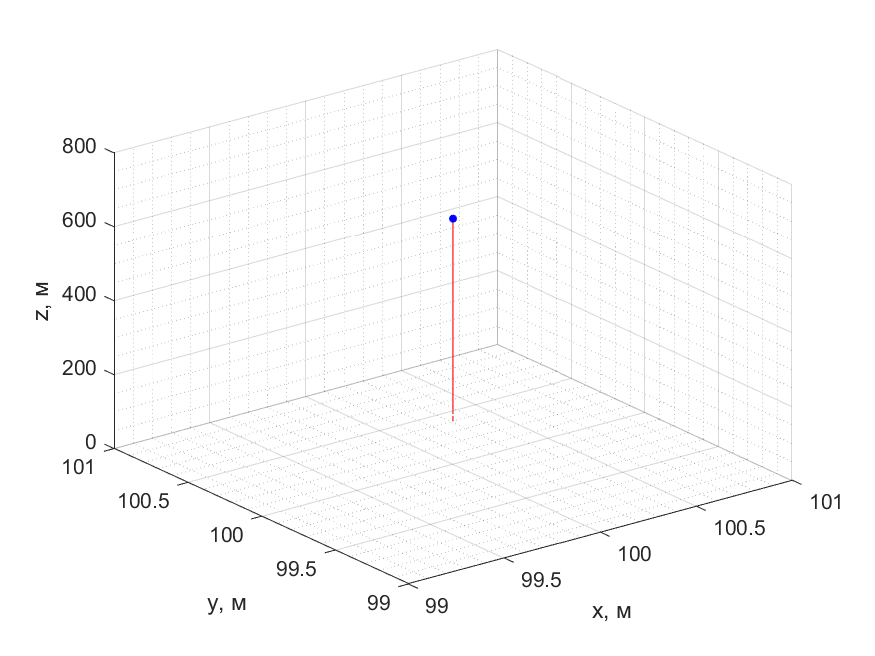
\includegraphics[width=0.75 \textwidth]{modeling_v_0_1_1.png}
    \caption{График моделирования квадрокоптера при входных напряжениях: \(U_1=5.5\)В, \(U_2=5.5\)В, \(U_3=5.5\)В, \(U_4=5.5\)В. Внешнее сопротивление отсутствует.}
    \label{fig:modeling-1}
\end{figure}

\begin{figure}[ht]
    \centering
    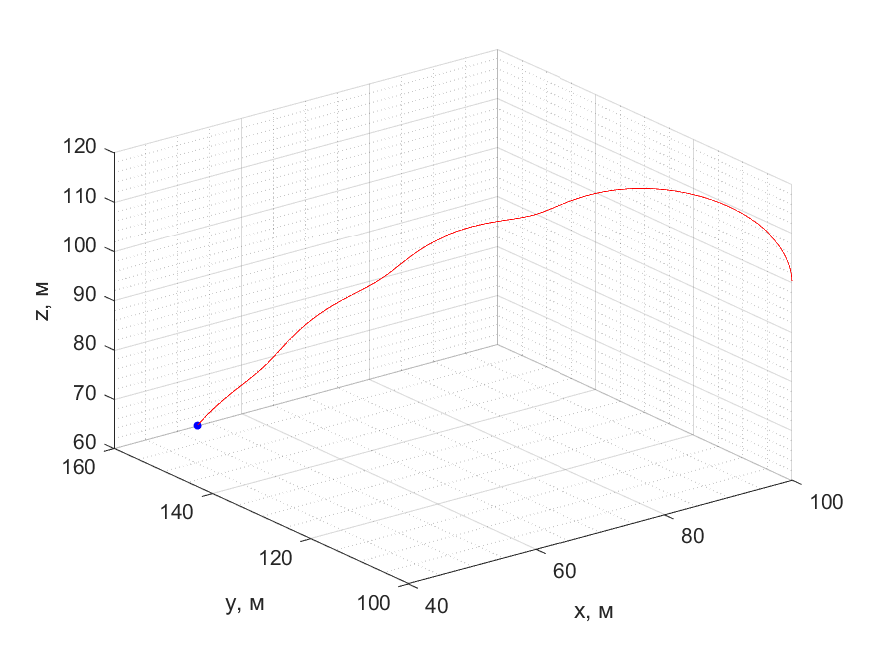
\includegraphics[width=0.75 \textwidth]{modeling_v_0_1_2.png}
    \caption{График моделирования квадрокоптера при входных напряжениях: \(U_1=5.5\)В, \(U_2=5.5\)В, \(U_3=0\)В, \(U_4=0\)В. Внешнее сопротивление отсутствует.}
    \label{fig:modeling-2}
\end{figure}

\begin{figure}[ht]
    \centering
    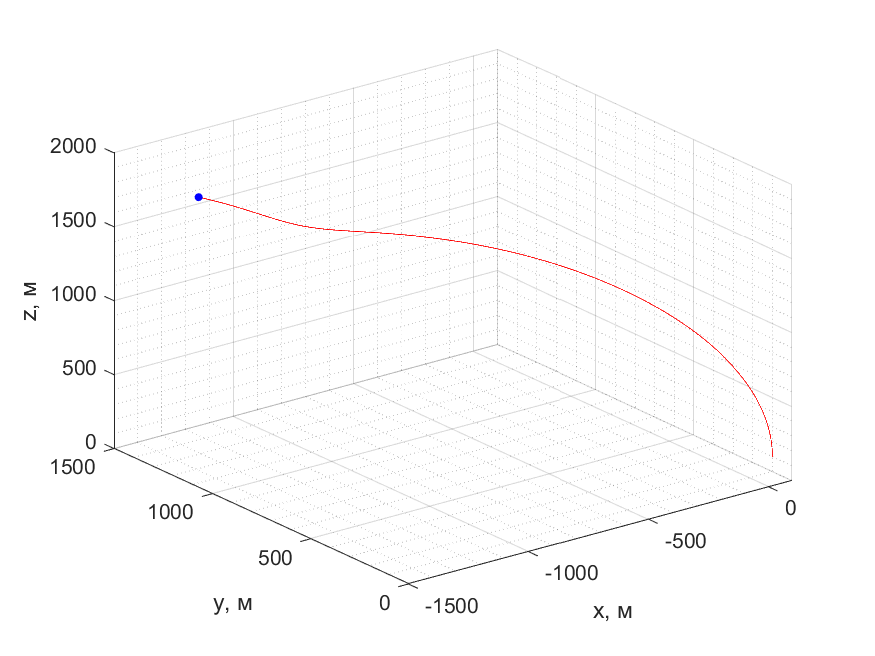
\includegraphics[width=0.8 \textwidth]{modeling_v_0_1_3.png}
    \caption{График моделирования квадрокоптера при входных напряжениях: \(U_1=5.5\)В, \(U_2=5.5\)В, \(U_3=5.4\)В, \(U_4=5.4\)В. Внешнее сопротивление отсутствует.}
    \label{fig:modeling-3}
\end{figure}

\begin{figure}[ht]
    \centering
    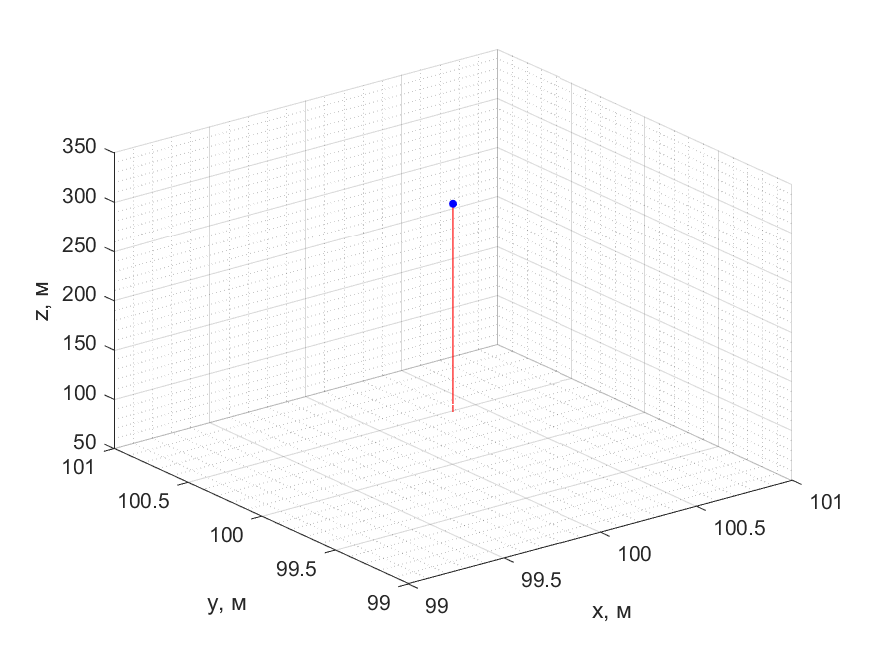
\includegraphics[width=0.8 \textwidth]{modeling_v_0_1_4.png}
    \caption{График моделирования квадрокоптера при входных напряжениях: \(U_1=5.5\)В, \(U_2=5.5\)В, \(U_3=5.5\)В, \(U_4=5.5\)В. Коэффициенты внешних сопротивлений \(C_a=C_b=0.1\), \(C_{drag}=1.1\).}
    \label{fig:modeling-4}
\end{figure}

\begin{figure}[ht]
    \centering
    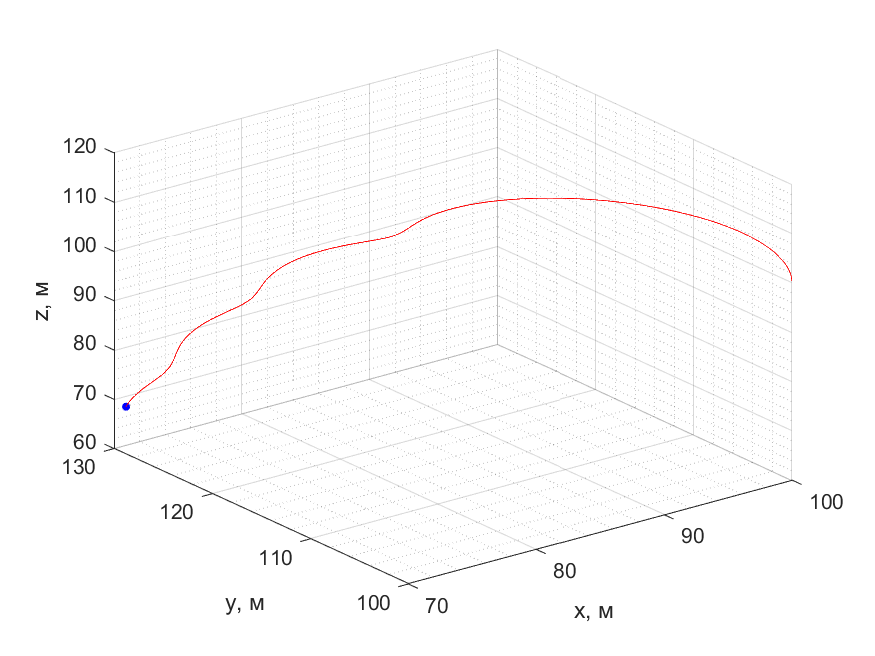
\includegraphics[width=0.8 \textwidth]{modeling_v_0_1_5.png}
    \caption{График моделирования квадрокоптера при входных напряжениях: \(U_1=5.5\)В, \(U_2=5.5\)В, \(U_3=0\)В, \(U_4=0\)В. Коэффициенты внешних сопротивлений \(C_a=C_b=0.1\), \(C_{drag}=1.1\).}
    \label{fig:modeling-5}
\end{figure}


\begin{figure}[ht]
    \centering
    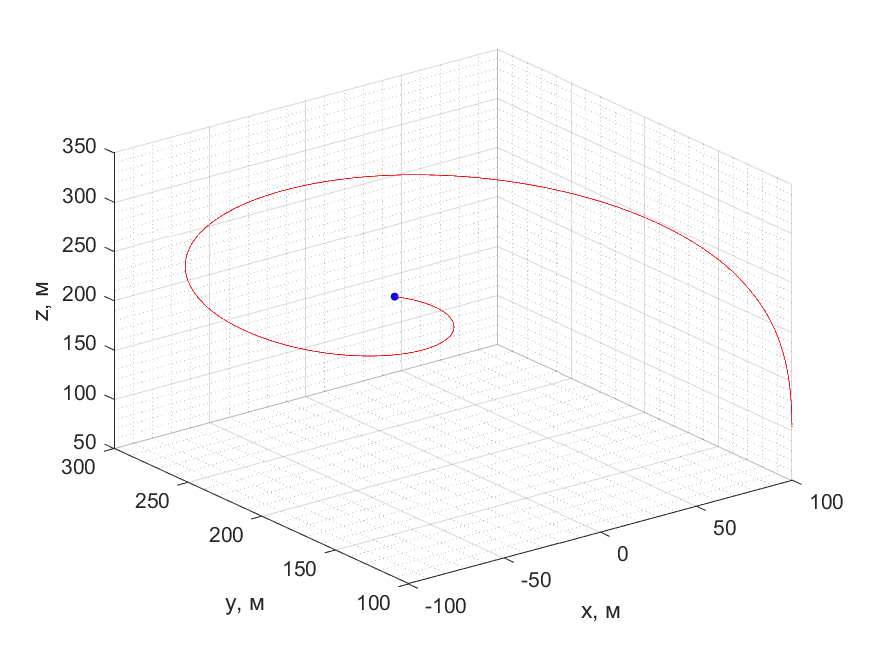
\includegraphics[width=0.8 \textwidth]{modeling_v_0_1_6.png}
    \caption{График моделирования квадрокоптера при входных напряжениях: \(U_1=5.5\)В, \(U_2=5.5\)В, \(U_3=5.4\)В, \(U_4=5.4\)В. Коэффициенты внешних сопротивлений \(C_a=C_b=0.1\), \(C_{drag}=1.1\).}
    \label{fig:modeling-6}
\end{figure}


\section{Моделирование в САПР Solidworks}

Также была создана модель квадрокоптера в САПР Solidworks.
Многие компоненты модели были найдены в интернете в свободном
доступе. В дальнейшем планируется добавить САПР модель
квадрокоптера в Simulink для более точного и наглядного 
моделирования.

\subsection{Фотографии квадрокоптера}

\begin{figure}[ht]
    \centering
    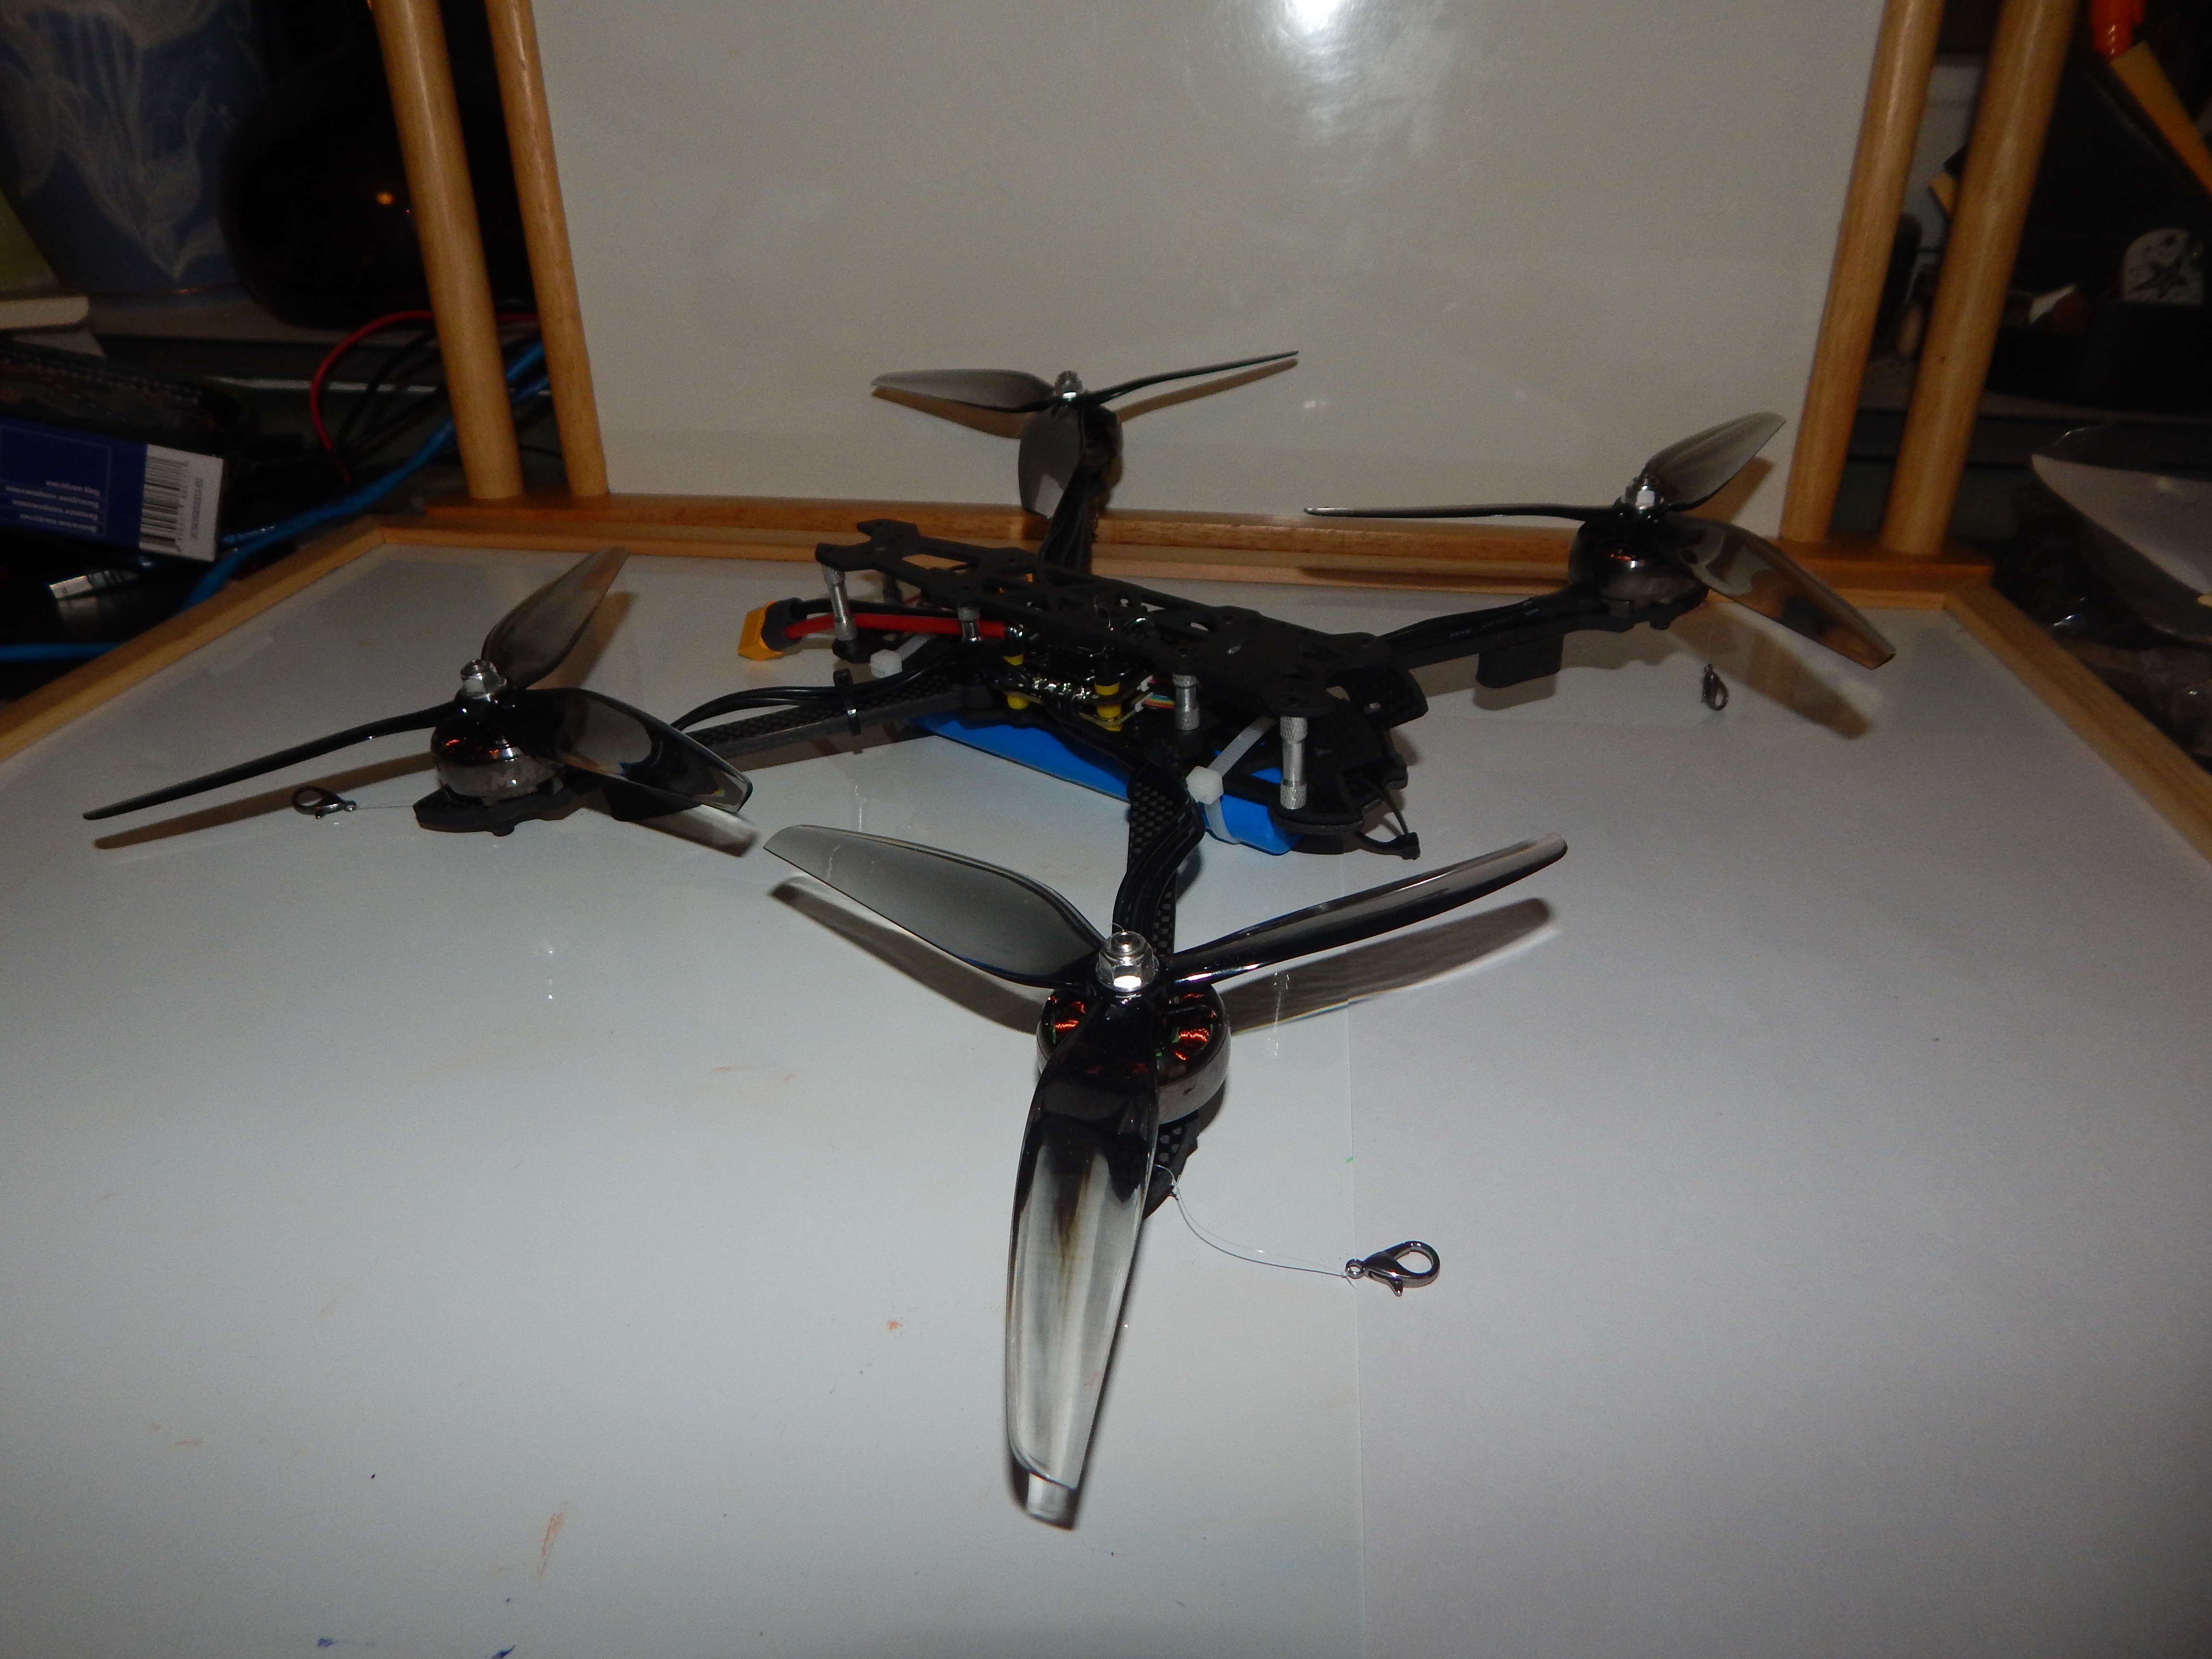
\includegraphics[width=0.8 \textwidth]{DSCN0425.JPG}
    \caption{Фотография квадрокоптера}
    \label{}
\end{figure}

\newpage

\subsection{Модель САПР}

\begin{figure}[ht]
    \centering
    \includegraphics[width=0.8 \textwidth]{cad-model-1.png}
    \caption{Модель квадрокоптера в Solidworks}
    \label{}
\end{figure}


\endinput % Моделирование для практики
%\chapter{}
\label{ch:chap1}

\section{Условие задания}
\label{sec:cond1}

\section{Расчеты}
\label{sec:calc1}

\endinput     % Библиографический поиск
\chapter{Разработка алгоритмов управления}
\label{ch:chap2}

\section{LQR регулятор по линеаризованной модели}

В качестве одного из базовых регуляторов можно использовать LQR регулятор по линеаризованной модели.
Для синтеза регулятора определим модель системы в форме вход-состояние-выход. 

Необходимо осуществлять управление по координатам \(r_x\), \(r_y\), \(r_z\) в соответствии с этим вектор
выхода системы будет выглядеть следующим образом:

\begin{equation}
Y = \begin{bmatrix}
    r_x \\
    r_y \\
    r_z
\end{bmatrix}.
\end{equation}


Система \eqref{eq:system} в матричном виде вход-состояние-выход будет выглядеть следующим образом:


\begin{equation}
    \begin{cases}
        \dot{X} = A X + B U + D;\\
        Y = C X.
    \end{cases}
\end{equation}


Вектор состояния расширен, добавлением положением по координатам \(r_x\), \(r_y\) и \(r_z\).

\begin{equation}
X = \begin{bmatrix} 
    r_x & 
    r_y & 
    r_z & 
    \dot{r}_x & 
    \dot{r}_y & 
    \dot{r}_z & 
    \phi &
    \theta & 
    \psi &
    \omega_{\phi} & 
    \omega_{\theta} & 
    \omega_{\psi} 
\end{bmatrix}^T.
\end{equation}

Вектор управления:

\begin{equation}
U = \begin{bmatrix}
    T \\
    \tau_\phi \\
    \tau_\theta \\
    \tau_\psi
\end{bmatrix}.
\end{equation}

\newpage
Матрица \(A\) будет выглядеть следующим образом:

\begin{equation}
    A=
\begin{bmatrix}
    0 & 0 & 0 & 1 & 0 & 0 & 0 & 0 & 0 & 0 & 0 & 0 \\
    0 & 0 & 0 & 0 & 1 & 0 & 0 & 0 & 0 & 0 & 0 & 0 \\
    0 & 0 & 0 & 0 & 0 & 1 & 0 & 0 & 0 & 0 & 0 & 0 \\
    0 & 0 & 0 & A_{drag_{1:1}} & A_{drag_{1:2}} & A_{drag_{1:3}} & 0 & 0 & 0 & 0 & 0 & 0 \\
    0 & 0 & 0 & A_{drag_{2:1}} & A_{drag_{2:2}} & A_{drag_{2:3}} & 0 & 0 & 0 & 0 & 0 & 0 \\
    0 & 0 & 0 & A_{drag_{3:1}} & A_{drag_{3:2}} & A_{drag_{3:3}} & 0 & 0 & 0 & 0 & 0 & 0 \\
    0 & 0 & 0 & 0 & 0 & 0 & 1 & T_\theta S_\phi & T_\theta C_\phi & 0 & 0 & 0 \\
    0 & 0 & 0 & 0 & 0 & 0 & 0 & C_\phi & -S_\phi & 0 & 0 & 0 \\
    0 & 0 & 0 & 0 & 0 & 0 & 0 & \frac{S_\phi}{C_\theta} & \frac{C_\phi}{C_\theta} & 0 & 0 & 0 \\
    0 & 0 & 0 & 0 & 0 & 0 & 0 & 0 & 0 & 0 & 0 & \frac{(I_z - I_y)\omega_{\theta}}{I_x} \\
    0 & 0 & 0 & 0 & 0 & 0 & 0 & 0 & 0 & 0 & 0 & \frac{(I_x - I_z)\omega_{\phi}}{I_y} \\
    0 & 0 & 0 & 0 & 0 & 0 & 0 & 0 & 0 & 0 & \frac{(I_y - I_x)\omega_{\phi}}{I_z} & 0
\end{bmatrix},
\end{equation}


где \(C_\phi = \cos\phi\), \(S_\phi = \sin\phi\), \(C_\theta = \cos\theta\), \(S_\theta = \sin\theta\),
\(T_\theta = \tan\theta\), матрица \(A_{drag}\):

\begin{equation}
A_{drag} = -\frac{T}{m} R (A_{ind} + A_{flap}) R^T - \frac{\rho C_{drag} S}{2m} \|\dot{r}\| I
.\end{equation}

Матрица \(B\):

\begin{equation}
B = \begin{bmatrix}
    0 & 0 & 0 & 0 \\
    0 & 0 & 0 & 0 \\
    0 & 0 & 0 & 0 \\
    \frac{\cos \psi \sin \theta \cos \phi + \sin \psi \sin \phi}{m} & 0 & 0 & 0 \\
    \frac{\sin \psi \sin \theta \cos \phi - \cos \psi \sin \phi}{m} & 0 & 0 & 0 \\
    \frac{\cos\theta\cos\phi}{m} & 0 & 0 & 0 \\
    0 & 0 & 0 & 0 \\
    0 & 0 & 0 & 0 \\
    0 & 0 & 0 & 0 \\
    0 & \frac{1}{I_x} & 0 & 0 \\
    0 & 0 & \frac{1}{I_y} & 0 \\
    0 & 0 & 0 & \frac{1}{I_z} \\
    \end{bmatrix}.
\end{equation}

\newpage

Матрица \(D\)

\begin{equation}
D = \begin{bmatrix}
    0 & 0 & 0 & 0 & 0 & -g & 0 & 0 & 0 & 0 & 0 & 0 \\
\end{bmatrix}^T.
\end{equation}

Матрица \(C\):

\begin{equation}
C = \begin{bmatrix}
    1 & 0 & 0 & 0 & 0 & 0 & 0 & 0 & 0 & 0 & 0 & 0 \\
    0 & 1 & 0 & 0 & 0 & 0 & 0 & 0 & 0 & 0 & 0 & 0 \\
    0 & 0 & 1 & 0 & 0 & 0 & 0 & 0 & 0 & 0 & 0 & 0 
\end{bmatrix}.
\end{equation}

\subsection{Линеаризация у точки равновесия}

Для синтеза LQR регулятора необходимо сначала линеаризовать квадрокоптер.

Производится линеаризация около точки равновесия, в которой угловые 
скорости и ускорения равны нулю. Состояние системы, которое будет соответствовать точке 
равновесия будет определяться следующим образом:

\begin{equation}
    \bar{X} = \begin{bmatrix}
        \bar{r}_x & \bar{r}_y & \bar{r}_z & 0 & 0 & 0 & 0 & 0 & \psi & 0 & 0 & 0 
    \end{bmatrix}.
    \label{eq:point1}
\end{equation}

Линеаризация системы у точки \eqref{eq:point1}:


\begin{equation}
    \bar{A} = 
    \begin{bmatrix}
    0 & 0 & 0 & 1 & 0 & 0 & 0 & 0 & 0 & 0 & 0 & 0 \\
    0 & 0 & 0 & 0 & 1 & 0 & 0 & 0 & 0 & 0 & 0 & 0 \\
    0 & 0 & 0 & 0 & 0 & 1 & 0 & 0 & 0 & 0 & 0 & 0 \\
    0 & 0 & 0 & \bar{A}_{drag_{1:1}} & \bar{A}_{drag_{1:2}} & \bar{A}_{drag_{1:3}} & 0 & 0 & 0 & 0 & 0 & 0 \\
    0 & 0 & 0 & \bar{A}_{drag_{2:1}} & \bar{A}_{drag_{2:2}} & \bar{A}_{drag_{2:3}} & 0 & 0 & 0 & 0 & 0 & 0 \\
    0 & 0 & 0 & \bar{A}_{drag_{3:1}} & \bar{A}_{drag_{3:2}} & \bar{A}_{drag_{3:3}} & 0 & 0 & 0 & 0 & 0 & 0 \\
    0 & 0 & 0 & 0 & 0 & 0 & 1 & 0 & 0 & 0 & 0 & 0 \\
    0 & 0 & 0 & 0 & 0 & 0 & 0 & 1 & 0 & 0 & 0 & 0 \\
    0 & 0 & 0 & 0 & 0 & 0 & 0 & 0 & 1 & 0 & 0 & 0 \\
    0 & 0 & 0 & 0 & 0 & 0 & 0 & 0 & 0 & 0 & 0 & 0 \\
    0 & 0 & 0 & 0 & 0 & 0 & 0 & 0 & 0 & 0 & 0 & 0 \\
    0 & 0 & 0 & 0 & 0 & 0 & 0 & 0 & 0 & 0 & 0 & 0
\end{bmatrix},
\end{equation}

где  

\begin{equation}
    \bar{A}_{drag} = - \frac{T}{m} (A_{ind} + A_{flap});
\end{equation}


\begin{equation}
    \bar{B} = \begin{bmatrix}
    0 & 0 & 0 & 0 \\
    0 & 0 & 0 & 0 \\
    0 & 0 & 0 & 0 \\
    0 & 0 & 0 & 0 \\
    0 & 0 & 0 & 0 \\
    \frac{1}{m} & 0 & 0 & 0 \\
    0 & 0 & 0 & 0 \\
    0 & 0 & 0 & 0 \\
    0 & 0 & 0 & 0 \\
    0 & \frac{1}{I_x} & 0 & 0 \\
    0 & 0 & \frac{1}{I_y} & 0 \\
    0 & 0 & 0 & \frac{1}{I_z} \\
    \end{bmatrix}.
\end{equation}

Матрицы \(C\) и \(D\) остаются без изменений.

LQR регулятор минимизирует критерий качества, который определяется как:

\begin{equation}
    J = \int_0^\infty \left( X^T Q X + U^T R U \right) dt.
\end{equation}

Для синтеза LQR регулятора необходимо определить матрицы \(Q\) и \(R\), которые определяют весовые коэффициенты для состояния и 
управления соответственно.
Пусть \(Q\) и \(R\) будут определены следующим образом:

\[
    Q = \begin{bmatrix}
        10 & 0 & 0 & 0 & 0 & 0 & 0 & 0 & 0 & 0 & 0 & 0 \\ %1
        0 & 10 & 0 & 0 & 0 & 0 & 0 & 0 & 0 & 0 & 0 & 0 \\ %2
        0 & 0 & 30 & 0 & 0 & 0 & 0 & 0 & 0 & 0 & 0 & 0 \\ %3
        0 & 0 & 0 & 0 & 0 & 0 & 0 & 0 & 0 & 0 & 0 & 0 \\ %4
        0 & 0 & 0 & 0 & 0 & 0 & 0 & 0 & 0 & 0 & 0 & 0 \\ %5
        0 & 0 & 0 & 0 & 0 & 0 & 0 & 0 & 0 & 0 & 0 & 0 \\ %6
        0 & 0 & 0 & 0 & 0 & 0 & 10 & 0 & 0 & 0 & 0 & 0 \\ %7
        0 & 0 & 0 & 0 & 0 & 0 & 0 & 10 & 0 & 0 & 0 & 0 \\ %8
        0 & 0 & 0 & 0 & 0 & 0 & 0 & 0 & 10 & 0 & 0 & 0 \\ %9
        0 & 0 & 0 & 0 & 0 & 0 & 0 & 0 & 0 & 0 & 0 & 0 \\    %10
        0 & 0 & 0 & 0 & 0 & 0 & 0 & 0 & 0 & 0 & 0 & 0 \\    %11
        0 & 0 & 0 & 0 & 0 & 0 & 0 & 0 & 0 & 0 & 0 & 0 \\    %12
    \end{bmatrix};
\]

\[
    R = \begin{bmatrix}
        1 & 0 & 0 & 0  \\ %1
        0 & 1 & 0 & 0 \\ %2
        0 & 0 & 1 & 0  \\ %3
        0 & 0 & 0 & 1
    \end{bmatrix}.
\]


Для обеспечения минимизации критерия качества \(J\) используется решение уравнения Риккати:

\begin{equation} 
    A^T P + P A - P B R^{-1} B^T P + Q = 0.
\end{equation}

Из этого уравнения можно получить \(P\) — матрица, с помощью которой можно найти матрицу \(K\) для LQR регулятора:

\begin{equation}
    K = R^{-1} B^T P.
\end{equation} 

Управление в системе будет осуществляться по следующему закону:
\begin{equation}
    U = -K X.
\end{equation}

Рассчитанные коэффициенты:

\[
    K =\begin{bmatrix}
        0 & 0 & 5.48 & 0 & 0 & 2.67 & 0 & 0 & 0 & 0 & 0 & 0 \\
        0 & -3.16 & 0 & 0 & -1.54 & 0 & 3.69 & 0 & 0 & 0.13 & 0 & 0 \\
        3.16 & 0 & 0 & 1.54 & 0 & 0 & 0 & 3.69 & 0 & 0 & 0.13 & 0 \\
        0 & 0 & 0 & 0 & 0 & 0 & 0 & 0 & 3.16 & 0 & 0 & 0.17
        \end{bmatrix}.
\]


\section{LQR регулятор с линеаризацией обратной связью}

В линеаризации обратной связью необходимо упростить уравнения квадрокоптера вводом 
новых виртуальных управлений. Управления будут выглядеть следующим образом:

% Без сопротивлений

\begin{equation}
    \begin{cases}
        \nu_x = \frac{1}{m} (\cos\phi \sin\theta  + \sin\psi \sin\phi) U_1;\\
        \nu_y = \frac{1}{m} (\sin\psi \sin\theta \cos\phi - \cos\psi \sin\phi) U_1;\\
        \nu_z = -g + \frac{1}{m} \cos\theta \cos\phi U_1;\\
        \nu_\phi = \frac{I_z - I_y}{I_x}\omega_\psi \omega_\theta + \frac{1}{I_x} U_2;\\
        \nu_\theta = \frac{I_x - I_z}{I_y}\omega_\phi \omega_\psi + \frac{1}{I_y} U_2;\\
        \nu_\psi = \frac{I_y - I_x}{I_z}\omega_\phi \omega_\theta + \frac{1}{I_z} U_2.
    \end{cases}
\end{equation}

Введение ошибок состояния:

\begin{equation}
\begin{aligned}
&\tilde{r}_x = r_x - r_x^d; \quad \tilde{v}_x = v_x - v_x^d; \\
&\tilde{r}_y = r_y - r_y^d; \quad \tilde{v}_y = v_y - v_y^d; \\
&\tilde{r}_z = r_z - r_z^d; \quad \tilde{v}_z = v_z - v_z^d; \\
&\tilde{\phi} = \phi - \phi^d; \quad \tilde{\omega}_\phi = \omega_\phi - \omega_\phi^d; \\
&\tilde{\theta} = \theta - \theta^d; \quad \tilde{\omega}_\theta = \omega_\theta - \omega_\theta^d; \\
&\tilde{\psi} = \psi - \psi^d; \quad \tilde{\omega}_\psi = \omega_\psi - \omega_\psi^d.
\end{aligned}
\end{equation}  

Динамика ошибок преобразуется в линейные подсистемы:  
\begin{equation}
\begin{cases} 
\dot{\tilde{r}}_x = \tilde{v}_x; \\
\dot{\tilde{v}}_x = \nu_x;
\end{cases}
\quad
\begin{cases} 
\dot{\tilde{r}}_y = \tilde{v}_y; \\
\dot{\tilde{v}}_y = \nu_y;
\end{cases}
\quad
\begin{cases} 
\dot{\tilde{r}}_z = \tilde{v}_z; \\
\dot{\tilde{v}}_z = \nu_z;
\end{cases}
\end{equation}
 
\begin{equation}
\begin{cases} 
\dot{\tilde{\phi}} = \tilde{\omega}_\phi; \\
\dot{\tilde{\omega}}_\phi = \nu_\phi;
\end{cases}
\quad
\begin{cases} 
\dot{\tilde{\theta}} = \tilde{\omega}_\theta; \\
\dot{\tilde{\omega}}_\theta = \nu_\theta;
\end{cases}
\quad
\begin{cases} 
\dot{\tilde{\psi}} = \tilde{\omega}_\psi; \\
\dot{\tilde{\omega}}_\psi = \nu_\psi.
\end{cases}
\end{equation}


Для каждой подсистемы применяется LQR регулятор:

\begin{equation}
    \begin{cases}
    \nu_x = -k_1^x \tilde{r}_x - k_2^x \tilde{v}_x; \\
    \nu_y = -k_1^y \tilde{r}_y - k_2^y \tilde{v}_y; \\
    \nu_z = -k_1^z \tilde{r}_z - k_2^z \tilde{v}_z; \\
    \nu_\phi = -k_1^\phi \tilde{\phi} - k_2^\phi \tilde{\omega}_\phi; \\
    \nu_\theta = -k_1^\theta \tilde{\theta} - k_2^\theta \tilde{\omega}_\theta; \\
    \nu_\psi = -k_1^\psi \tilde{\psi} - k_2^\psi \tilde{\omega}_\psi.
    \end{cases}
\end{equation}

Для подсистеме по координате \(r_x\) синтез LQR регулятор выглядит следующим образом:
Матрицы состояния и управления:

\begin{equation}
    A_x=\begin{bmatrix}
    0 & 1 \\
    0 & 0
\end{bmatrix}, \quad
B_x = \begin{bmatrix}
    0 \\
    1
\end{bmatrix}.\end{equation}

Осуществляется выбор матриц \(Q\) и \(R\) для критерия качества. 
И решается уравнение Риккати:

\begin{equation}
    A_x^T P + P A_x - P B_x R^{-1} B_x^T P + Q = 0.
\end{equation}

Откуда получаем коэффициенты \(k_1^x\) и \(k_2^x\):
\begin{equation}
    k^x = R^{-1} B_x^T P.
\end{equation}

Аналогично синтезируются регуляторы для остальных подсистем.

Полученные виртуальные управления обратно преобразуются в реальные управления:

\begin{equation}
    \begin{cases}
        \bar{\phi} = \frac{v_x}{v_z+g};\\
        \bar{\theta} =  \frac{v_y}{v_z+g};
    \end{cases}
\end{equation}

\begin{equation}
    \begin{cases}
    U_1 = \frac{m (\nu_z + g)}{\cos\bar{\phi} \cos\bar{\theta}}; \\
    U_2 = I_x \nu_\phi - (I_y - I_z) \omega_\theta \omega_\psi; \\
    U_2 = I_y \nu_\theta - (I_x - I_z) \omega_\phi \omega_\psi; \\
    U_4 = I_z \nu_\psi - (I_x - I_y) \omega_\phi \omega_\theta.
    \end{cases}
\end{equation}
% С сопротивлениями
Для управлений были выбраны различные матрицы \(Q\) и \(R\), полученные коэффициенты регулятора:

\[
K = \begin{bmatrix}
    5  & 5  &  3  & 141 & 141 & 0 \\
    10 & 10 &  3  & 1000 & 1000 & 0 
\end{bmatrix}^T.
\]


\section{Nonlinear MPC}

Nonlinear MPC --- один из самых эффективных регуляторов с точки зрения оптимизации управления и 
точности. Суть регулятора довольно простая, на вход поступает вектор состояний квадрокоптера 
и желаемое состояние на некоторое количество 
шагов вперед. Количество шагов называется горизонтом предсказания. Далее 
внутри регулятора происходит моделирование поведение квадрокоптера с управлением, которое может быть
изначально проинициализировано или получено с предыдущего шага.
Затем происходит минимизация заданного критерия качества, который обычно имеет следующий вид:

\begin{equation}
    J = \sum_{k=0}^{N-1} \left( e_k^T Q e_k + u_k^T R u_k \right),
\end{equation}

где \(X_k\) — состояние системы на \(k\)-м шаге, \(X_k^d\) — желаемое состояние на \(k\)-м шаге, \(U_k\) — управление на \(k\)-м шаге, \(Q\) и \(R\) — весовые матрицы, определяющие важность отклонения состояния и управления соответственно, \(N\) — горизонт предсказания.

Минимизация критерия качества осуществляется с учетом ограничений на динамику системы, которые задаются в виде:

\begin{equation}
    X_{k+1} = f(X_k, U_k),
\end{equation}

где \(f(X_k, U_k)\) — нелинейная модель квадрокоптера, а также ограничений на управление и состояния, например:

\begin{equation}
    U_{\text{min}} \leq U_k \leq U_{\text{max}}, \quad X_{\text{min}} \leq X_k \leq X_{\text{max}}.
\end{equation}

Решение задачи оптимизации дает последовательность управлений \(\{U_0, U_1, \dots, U_{N-1}\}\), из которых на выходе регулятора используется только первое управление \(U_0\). Это управление подается на квадрокоптер, после чего процесс повторяется на следующем временном шаге с обновленным состоянием системы.


Регулятор можно расширять и модифицировать, можно ввести ограничения, штрафные стоимости за быстрые переключения управления,
изменить модель объекта, например учитывать характер внешних возмущений.


В среде Matlab/Simulink есть реализация Nonlinear MPC регулятора, но в текущей работе было принято решение полностью написать 
функцию Nonlinear MPC регулятора с введением некоторых модификаций, и чтобы в дальнейшем было проще перенести 
реализацию на реальную систему.

Система управления не разделена на контуры, 
и реализует вышеописанную логику. Схема регулятора представлена на рисунке \ref{fig:mpc-1}. 
Для минимизации критерия \(J\) используется градиентный спуск, в математическом представлении:

\begin{equation}
    U_{k+1} = U_k - \nabla J(U_k).
\end{equation}

Также введены дополнительные мягкие ограничения на углы \(\phi\) и \(\theta\), чтобы квадрокоптер
не переворачивался в воздухе.

\begin{figure}[ht]
    \centering
    \includegraphics[width=0.8 \textwidth]{mpc-1.png}
    \caption{Схема регулятора Nonlinear MPC}
    \label{fig:mpc-1}
\end{figure}


\endinput     % Вывод законов управления

\includepdf[pages={2-7}]{/home/shulc/shulc/DroneModel/Articles/15_LQR_2_linearization.pdf}
%\chapter{}
\label{ch:chap3}

\section{}
\label{sec:cond3}


\endinput     % Моделирование
%\chapter{Реализация квадрокоптера на базе STM32F722}

Основной задачей являлась 
реализация эффективной системы стабилизации и управления 
полетом с использованием линейного квадратичного регулятора LQR 
с линеаризацией обратной связью. Выбор 
LQR был обусловлен его хорошим соотношением между вычислительной 
нагрузкой и качеством управления, что видно 
по результатам моделирования приведенным в предыдущей главе.

\section{Аппаратная часть квадрокоптера}

В результате разработан квадрокоптер, построенный на базе готового 
полетного контроллера Radiolink F722, в основе которого лежит 
микроконтроллер STM32F722\cite{RadiolinkF722}\cite{STM32F722}. 
Полетный контроллер Radiolink F722 включает в себя встроенный датчик пространственного положения 
и гироскопа ICM42688-P. Взаимодействие с датчиком осуществлялось по интерфейсу SPI\cite{ICM42688P}.


\begin{figure}[ht]
    \centering
    \includegraphics[width=0.3 \textwidth]{flight-controller-1.png}
    \caption{Полетный контроллер Radiolink F722}
    \label{}
\end{figure}

Управление четырьмя моторами осуществлялось с помощью широтно-импульсной модуляции
через электронные регуляторы скорости(ESC). На квадрокоптер были установлены популярные бесколлектрные моторы
EMAX ECO || 2306 1300 KV\cite{EmaxECO1300KV}. KV --- это стандартная характеристика бесколлекторных моторов, которое означает
количество оборотов на вольт без нагрузки.

\begin{figure}[ht]
    \centering
    \includegraphics[width=0.45 \textwidth]{motor-1.png}
    \caption{Мотор EMAX ECO || 2306 1300 KV}
    \label{}
\end{figure}


В качестве рамы квадрокоптера было выбрано готовое решение --- корпус Mark 4 295 мм.

\begin{figure}[ht]
	\centering
	\includegraphics[width=0.8 \textwidth]{drone.JPG}
	\caption{Квадрокоптер в собранном виде}
	\label{}
\end{figure}


В среде САПР среде Solidworks была реализована 3D модель квадрокоптера. Эта модель была
импортирована в среду Matlab/Simulink для имитационного моделирования.

\begin{figure}[ht]
	\centering
	\includegraphics[width=0.8 \textwidth]{cad-model-1.png}
	\caption{3D модель квадрокоптера в Solidworks}
	\label{}
\end{figure}

\section{Программное обеспечение квадрокоптера}

Разработка программного обеспечения велась в среде 
STM32CubeIDE. Предварительно были изучены исходные файлы открытой 
прошивки полетных контроллеров Betaflight, благодаря которым удалось произвести
обратное проектирование полетного контроллера для разработки собственного программного обеспечения\cite{Betaflight}.

Для удобной и универсальной коммуникации с квадрокоптером была выбрана коммуникация по 
протоколу MQTT, который часто используется в проектах интернет вещей в сетях 
с низкой пропускной способностью\cite{MQTT}. Таким образом сообщения доходят быстро и довольно стабильно
при должной настройке. Так как микроконтроллер STM32F722 не оснащен WI-FI модулем к нему 
был подключен микроконтроллер ESP8266, который обладает встроенным WI-FI модулем и способен 
принимать команды по MQTT, передавая их на STM32F722 по интерфейсу UART.

\begin{figure}[ht]
	\centering
\hspace*{\fill}%
	\begin{subfigure}[b]{0.49\textwidth}
        \centering
		\includegraphics[height=9cm,keepaspectratio]{esp8266.png}
		\caption{}
		\label{fig:tiger1}
	\end{subfigure}
\hfill
	\begin{subfigure}[b]{0.49\textwidth}
        \centering
		\includegraphics[height=9cm,keepaspectratio]{drone-inside-1.png}
        \caption{}
		\label{fig:tiger2}
	\end{subfigure}
\hspace*{\fill}%
	\caption{На рисунке (а) ESP8266. На рисунке (б)Встроенный ESP8266 на квадрокоптере}
	\label{fig:tiger}
\end{figure}

\newpage

Также был сделана панель управления для управления квадрокоптером через окно
браузера. 


\begin{figure}[ht]
	\centering
\hspace*{\fill}%
	\begin{subfigure}[b]{0.49\textwidth}
        \centering
		\includegraphics[height=9cm,keepaspectratio]{dashboard-1.png}
		\caption{}
		\label{fig:tiger1}
	\end{subfigure}
\hfill
	\begin{subfigure}[b]{0.49\textwidth}
        \centering
		\includegraphics[height=9cm,keepaspectratio]{dashboard-2.png}
        \caption{}
		\label{fig:tiger2}
	\end{subfigure}
\hspace*{\fill}%
	\caption{Панель управления квадрокоптером в браузере}
	\label{fig:tiger}
\end{figure}

В качестве брокера сообщений для обеспечения передачи команд от компьютера к 
микроконтроллеру ESP8266 был выбран популярный - Mosquitto, который можно развернуть 
локальной машине\cite{Mosquitto}.

\newpage

\section{Локализация квадрокоптера}

Для решения задачи локализации квадрокоптера было решено использовать визуальные маркеры apriltag\cite{AprilTag}.
В библиотеке OpenCV уже есть встроенные функции для детектирования и отслеживания маркеров apriltag\cite{OpenCV}\cite{Aruco}.
Были также написана логика для калибровки камеры для получения координат 
 по осям: X, Y, Z в системе СИ. Код приложения для отслеживания визуального маркера 
запускался на одноплатном компьютере Raspberry PI 4b с 4 Гб оперативной памяти. 
Использовалась камера Raspberry Pi Camera Module Rev 1.3 с разрешением 5 мегапикселей.
На каждом кадре осуществляется поиск маркера, рассчитанные координаты отправляются по
MQTT на квадрокоптер.


\begin{figure}[ht]
    \centering
    \includegraphics[width=0.5 \textwidth]{drone-apriltag.png}
    \caption{Apriltag 36h11 закрепленный на квадрокоптере}
    \label{}
\end{figure}

\begin{figure}[ht]
	\centering
\hspace*{\fill}%
	\begin{subfigure}[b]{0.49\textwidth}
        \centering
		\includegraphics[height=9cm,keepaspectratio]{camera+drone_1.png}
		\caption{}
		\label{fig:tiger1}
	\end{subfigure}
\hfill
	\begin{subfigure}[b]{0.49\textwidth}
        \centering
		\includegraphics[height=9cm,keepaspectratio]{camera+drone_2.png}
        \caption{}
		\label{fig:tiger2}
	\end{subfigure}
\hspace*{\fill}%
	\caption{Детектирование тэга на камере}
	\label{fig:tiger}
\end{figure}

\newpage


\section{Тестирование квадрокоптера}

Разработанный прототип частично тестировался в полевых условиях на двух стендах и в свободном полете.


\begin{figure}[ht]
    \centering
    \includegraphics[width=0.5 \textwidth]{drone_fly_1.png}
    \caption{Тестирование квадрокоптера в свободном полете}
    \label{}
\end{figure}

\begin{figure}[ht]
	\centering
\hspace*{\fill}%
	\begin{subfigure}[b]{0.49\textwidth}
        \centering
		\includegraphics[height=9cm,keepaspectratio]{test-2.png}
		\caption{}
		\label{fig:tiger1}
	\end{subfigure}
\hfill
	\begin{subfigure}[b]{0.49\textwidth}
        \centering
		\includegraphics[height=9cm,keepaspectratio]{test-1.png}
        \caption{}
		\label{fig:tiger2}
	\end{subfigure}
\hspace*{\fill}%
	\caption{Тестирование квадрокоптера на стендах}
	\label{fig:tiger}
\end{figure}

Тестирование на предмет слежения за траекторией не удалось в силу трудностей с построением специального полигона, 
однако
регулятор показал свою работоспособность в решении задачи стабилизации 
квадрокоптера. 


\endinput
%\chapter*{Заключение}
\addcontentsline{toc}{chapter}{Заключение}
\label{ch:chap1}

В рамках выполнения работы были достигнуты поставленные цели: 
разработаны алгоритмы управления квадрокоптером для слежения за траекторией, 
проведено их моделирование в среде MATLAB/Simulink, выполнено сравнение 
качества переходных процессов, наиболее эффективный алгоритм 
реализован на реальном квадрокоптере.

Проведённое моделирование системы управления дроном на траекториях `восьмёрка' и `куб' 
позволило оценить эффективность трёх регуляторов: классического LQR, LQR с 
линеаризацией обратной связью (LQR+FB) и нелинейного MPC. Наибольшую точность 
демонстрируют регуляторы LQR+FB и MPC. Например, для траектории «восьмёрка» 
RMSE положения по осям X и Y у MPC составили 0.463 м и 0.305 м соответственно, 
что близко к результатам LQR+FB (0.470 м и 0.324 м). При этом MPC обеспечил минимальную
 ошибку по высоте (0.501 м), что подтверждает его преимущество в условиях отсутствия возмущений.

Регулятор LQR+FB показал значительно более высокую скорость моделирования 
благодаря меньшей вычислительной сложности по сравнению с MPC. 
Но нужно отметить, что регулятор MPC обладает высокой расширяемостью и 
конфигурируемостью. Возможность 
учёта нелинейностей, ограничений на состояния и управления, 
а также адаптация к агрессивным маневрам открывают перспективы 
для дальнейшего улучшения точности. Однако его реализация 
требует значительных вычислительных ресурсов, что может ограничивать применение в реальном времени.

В связи с отмеченными недостатками MPC регулятора было решено использовать
LQR регулятор с линеаризацией обратной связью для экспериментов на реальном квадрокоптере.
В ходе разработки квадрокоптера было реализовано следующее: программное обеспечение для квадрокоптера на
базе микроконтроллера STM32F722;
система коммуникации с квадрокоптером посредством MQTT протокола и микроконтроллера ESP8266; 
панель управления для браузера; система локализации с использованием визуальных маркеров
apriltag. Было проведено тестирование регулятора для стабилизации квадрокоптера на двух стендах. 

Выбор регулятора зависит от условий задачи и располагаемых ресурсов, соответственно 
LQR с линеаризацией обратной связью
будет очень хорошим и эффективным регулятором для решения многих задач, 
но MPC будет лучшим выбором, если есть большие вычислительные мощности и временные ресурсы для 
настройки параметров и модификации регулятора. 

\endinput

%\nocite{*}
%\printbibliography[title=Список использованных источников]
%\chapter{Приложение А}

Листинг кода основной программы STM32F722.

\begin{lstlisting}[language=C++]
#include "main.h"
#include "usb_device.h"

/* Private includes ----------------------------------------------------------*/
/* USER CODE BEGIN Includes */
#include <stdio.h>
#include "usbd_cdc_if.h"
#include <icm4268.h>
#ifndef MATH
#include <math.h>
#define MATH
#endif
//#include "ICM42688.h"
/* USER CODE END Includes */

/* Private typedef -----------------------------------------------------------*/
/* USER CODE BEGIN PTD */

/* USER CODE END PTD */

/* Private define ------------------------------------------------------------*/
/* USER CODE BEGIN PD */
typedef enum {
    DRONE_STATE_IDLE = 0,
    DRONE_STATE_TEST_CYCLE,
    DRONE_STATE_EMERGENCY_STOP,
    DRONE_STATE_LANDING,
    DRONE_STATE_LQR,
    DRONE_STATE_MOVE_FORWARD,
    DRONE_STATE_HOVER,
    DRONE_TEST_DIRS,
} DroneState;
volatile DroneState currentState = DRONE_STATE_IDLE;
volatile DroneState requestedState = DRONE_STATE_IDLE;
volatile uint32_t stateStartTime = 0;
volatile uint32_t landingStartAltitude = 0;
volatile uint8_t landingInProgress = 0;
/* USER CODE END PD */

/* Private macro -------------------------------------------------------------*/
/* USER CODE BEGIN PM */
#define RX_BUF_SIZE  16
static uint8_t rx_byte;
static char cmd_buf[RX_BUF_SIZE];
static uint8_t cmd_idx = 0;
static uint8_t mode = 0;
uint8_t rx_buf[5];
volatile uint8_t rx_idx = 0;
GPIO_TypeDef* ICM_CS_GPIO_Port = GPIOB;
uint16_t      ICM_CS_Pin       = GPIO_PIN_2;
float angles_rad[3], angles_deg[3], gyro_rad_s[3], angles_speed[3], angles_rad_prev[3];
int16_t accel_raw[3], gyro_raw[3];
float filtered_accel[3] = {0};
float filtered_gyro[3] = {0};
float dt = 0.01f;
float pos[3], prev_pos[3], pos_req[3], speed[3];
float k1=10,k2=5,k3=10,k4=5,k5=10,k6=5,k7=31623,k8=251,k9=31623,k10=251,k11=0,k12=0;
int requested_speed = 1220;
float m = 0.65, Ix=0.0021, Iy=0.0021, Iz=0.0043;
float kf=0.0000158, k_1_2_l=3.33, kf_inv=63463.8;
uint16_t motorPWM[4];
const float scale = 0.15f;
const float min_pwm = 1140.0f;
const float max_pwm = 1500.0f;
float bias[3];
uint32_t timer_lqr = 0;
/* USER CODE END PM */

/* Private variables ---------------------------------------------------------*/

SPI_HandleTypeDef hspi1;

TIM_HandleTypeDef htim2;
TIM_HandleTypeDef htim3;
TIM_HandleTypeDef htim4;
DMA_HandleTypeDef hdma_tim2_ch1;
DMA_HandleTypeDef hdma_tim2_ch2_ch4;
DMA_HandleTypeDef hdma_tim3_ch1_trig;
DMA_HandleTypeDef hdma_tim4_ch1;

UART_HandleTypeDef huart3;

/* USER CODE BEGIN PV */

/* USER CODE END PV */

/* Private function prototypes -----------------------------------------------*/
void SystemClock_Config(void);
static void MPU_Config(void);
static void MX_GPIO_Init(void);
static void MX_DMA_Init(void);
static void MX_TIM2_Init(void);
static void MX_TIM3_Init(void);
static void MX_TIM4_Init(void);
static void MX_SPI1_Init(void);
static void MX_USART3_UART_Init(void);
/* USER CODE BEGIN PFP */
/* USER CODE END PFP */

/* Private user code ---------------------------------------------------------*/
/* USER CODE BEGIN 0 */
void USB_CDC_RxHandler(uint8_t*, uint32_t);
int _write(int file, char *ptr, int len) {
    CDC_Transmit_FS((uint8_t*) ptr, len); return len;
}
void SetMotorOutputs(uint16_t ch1, uint16_t ch2, uint16_t ch3, uint16_t ch4)
{
    __HAL_TIM_SET_COMPARE(&htim2, TIM_CHANNEL_1, ch1);
    __HAL_TIM_SET_COMPARE(&htim2, TIM_CHANNEL_2, ch2);
    __HAL_TIM_SET_COMPARE(&htim3, TIM_CHANNEL_1, ch3);
    __HAL_TIM_SET_COMPARE(&htim4, TIM_CHANNEL_1, ch4);
}
void ArmESCs(void)
{
    SetMotorOutputs(1000, 1000, 1000, 1000);
    HAL_Delay(2000);
}
void testCycle(void){
    for (uint16_t dc = 1000; dc <= 1220; dc += 2) {
        SetMotorOutputs(dc, dc, dc, dc);
        HAL_Delay(80);
    }
    for (uint16_t dc = 1220; dc > 1000; dc -= 2) {
        SetMotorOutputs(dc, dc, dc, dc);
        HAL_Delay(80);
    }
    //SetMotorOutputs(1000, 1000, 1000, 1000);
}
void testMotorsDirs(void){
    SetMotorOutputs(1150, 1000, 1000, 1000);
    HAL_Delay(2500);
    SetMotorOutputs(1000, 1000, 1000, 1000);
    ///////////
    SetMotorOutputs(1000, 1150, 1000, 1000);
    HAL_Delay(2500);
    SetMotorOutputs(1000, 1000, 1000, 1000);
    /////////
    SetMotorOutputs(1000, 1000, 1150, 1000);
    HAL_Delay(2500);
    SetMotorOutputs(1000, 1000, 1000, 1000);
    ////////
    SetMotorOutputs(1000, 1000, 1000, 1150);
    HAL_Delay(2500);
    SetMotorOutputs(1000, 1000, 1000, 1000);
}
void stopMotors(void){
    //SetMotorOutputs(dc, dc, dc, dc);
    SetMotorOutputs(1000, 1000, 1000, 1000);
}
void performLanding(void) {
    static uint32_t landingTimer = 0;
    static uint16_t currentThrottle = 0;

    if (!landingInProgress) {
    landingInProgress = 1;
    landingTimer = HAL_GetTick();
    currentThrottle = 1200;
    printf("LANDING STARTED\r\n");
    }

    uint32_t elapsedTime = HAL_GetTick() - landingTimer;
    if (elapsedTime < 5000) {
    uint16_t newThrottle = 1000 + (uint16_t)((float)(currentThrottle - 1000) * (1.0f - (float)elapsedTime / 5000.0f));
    SetMotorOutputs(newThrottle, newThrottle, newThrottle, newThrottle);
    } else {
    SetMotorOutputs(1000, 1000, 1000, 1000);
    landingInProgress = 0;
    currentState = DRONE_STATE_IDLE;
    printf("LANDING COMPLETE\r\n");
    }
}

void performTestCycle(void) {
    static uint16_t currentDC = 1000;
    static uint8_t increasing = 1;
    static uint32_t lastUpdate = 0;

    if (requestedState != currentState) {
    return;
    }

    uint32_t now = HAL_GetTick();
    if (now - lastUpdate >= 80) {
    lastUpdate = now;

    if (increasing) {
        currentDC += 2;
        if (currentDC >= requested_speed)
        increasing = 0;
    } else {
        currentDC -= 2;
        if (currentDC <= 1020) {
        increasing = 1;
        currentState = DRONE_STATE_IDLE;
        requestedState = DRONE_STATE_IDLE;
        SetMotorOutputs(1000, 1000, 1000, 1000);
        printf("TEST CYCLE COMPLETE\r\n");
        return;
        }
    }

    SetMotorOutputs(currentDC, currentDC, currentDC, currentDC);
    }
}


void performLQRStable(void) {
    float LQR_SPEED[4] = {0, 0, 0, 0};

    if (requestedState != currentState) {
    return;
    }
    uint32_t now = HAL_GetTick();
    if (timer_lqr<now){
        float nu[6];
        nu[0] = -k1*(pos[0]-pos_req[0])-k2*speed[0];
        nu[1] = -k3*(pos[1]-pos_req[1])-k4*speed[1];
        nu[2] = -k5*(pos[2]-pos_req[2])-k6*speed[2];

        nu[5] = -k11*angles_rad[2]-k12*angles_speed[2];
        //uint32_t now = HAL_GetTick();
        float bar_phi = atan2f(nu[0], (nu[2]+9.81f));
        float bar_theta = atan2f(nu[1], (nu[2]+9.81f));

        nu[3] = -k7*(angles_rad[0]-bar_phi)-k8*angles_speed[0];
        nu[4] = -k9*(angles_rad[1]-bar_theta)-k10*angles_speed[1];

        float U[4];
        U[0] = m*(nu[2]+9.81)/(cosf(bar_phi)*cosf(bar_theta));
        U[1] = Ix*nu[3]-(Iy-Iz)*angles_speed[1]*angles_speed[2];
        U[2] = Iy*nu[4]-(Ix-Iz)*angles_speed[0]*angles_speed[2];
        U[3] = Iz*nu[5]-(Ix-Iy)*angles_speed[0]*angles_speed[1];
        float temps[4];
        temps[0] = kf_inv*(U[0]-k_1_2_l*U[2])-U[3];
        temps[1] = kf_inv*(U[0]-k_1_2_l*U[1])+U[3];
        temps[2] = kf_inv*(U[0]+k_1_2_l*U[2])-U[3];
        temps[3] = kf_inv*(U[0]+k_1_2_l*U[1])+U[3];
        printf("WORING\r\n");
//	  for (int i = 0; i < 4; i++) {
//		if (temps[i]<0){
//			printf("ERROR ZERO CROSSING IN SQRT\r\n");
//			return;
//		}
//	  }
        LQR_SPEED[0] = 0.5*sqrtf(temps[0]);
        LQR_SPEED[1] = 0.5*sqrtf(temps[1]);
        LQR_SPEED[2] = 0.5*sqrtf(temps[2]);
        LQR_SPEED[3] = 0.5*sqrtf(temps[3]);
        for (int i = 0; i < 4; i++) {
            float pwm = LQR_SPEED[i] * scale + min_pwm;

            pwm = fmaxf(pwm, min_pwm);
            pwm = fminf(pwm, max_pwm);

            motorPWM[i] = (uint16_t)pwm;
        }
        printf("motors: %d, %d, %d, %d\r\n", motorPWM[0], motorPWM[1],motorPWM[2],motorPWM[3]);

        SetMotorOutputs(motorPWM[3],motorPWM[2],motorPWM[0], motorPWM[1]);
    }

}

void handleDroneState(void) {
    if (requestedState != currentState) {
    switch (requestedState) {
        case DRONE_STATE_EMERGENCY_STOP:
        SetMotorOutputs(1000, 1000, 1000, 1000);
        printf("EMERGENCY STOP ACTIVATED\r\n");
        break;

        case DRONE_STATE_LANDING:
        landingInProgress = 0;
        break;

        case DRONE_STATE_TEST_CYCLE:
        printf("TEST CYCLE STARTED\r\n");
        break;

        case DRONE_STATE_LQR:
            timer_lqr = HAL_GetTick()+2500;
            printf("STARTED LQR\r\n");
            break;

        default:
        break;
    }

    currentState = requestedState;
    stateStartTime = HAL_GetTick();
    }

    switch (currentState) {
    case DRONE_STATE_IDLE:
        break;

    case DRONE_STATE_TEST_CYCLE:
        performTestCycle();
        break;

    case DRONE_STATE_LANDING:
        performLanding();
        break;

    case DRONE_STATE_EMERGENCY_STOP:
        SetMotorOutputs(1000, 1000, 1000, 1000);
        break;

    case DRONE_STATE_LQR:
        performLQRStable();
        break;

    default:
        break;
    }
}

/* USER CODE END 0 */

/**
    * @brief  The application entry point.
    * @retval int
    */
int main(void)
{

    /* USER CODE BEGIN 1 */

    /* USER CODE END 1 */

    /* MPU Configuration--------------------------------------------------------*/
    MPU_Config();

    /* MCU Configuration--------------------------------------------------------*/

    /* Reset of all peripherals, Initializes the Flash interface and the Systick. */
    HAL_Init();

    /* USER CODE BEGIN Init */

    /* USER CODE END Init */

    /* Configure the system clock */
    SystemClock_Config();

    /* USER CODE BEGIN SysInit */

    /* USER CODE END SysInit */

    /* Initialize all configured peripherals */
    MX_GPIO_Init();
    MX_DMA_Init();
    MX_USB_DEVICE_Init();
    MX_TIM2_Init();
    MX_TIM3_Init();
    MX_TIM4_Init();
    MX_SPI1_Init();
    MX_USART3_UART_Init();
    /* USER CODE BEGIN 2 */
    HAL_TIM_PWM_Start(&htim2, TIM_CHANNEL_1);
    HAL_TIM_PWM_Start(&htim2, TIM_CHANNEL_2);
    HAL_TIM_PWM_Start(&htim3, TIM_CHANNEL_1);
    HAL_TIM_PWM_Start(&htim4, TIM_CHANNEL_1);
    ArmESCs();
    //TestSPI();
    if (ICM_Init() != HAL_OK) {
        HAL_Delay(1000);
        printf("ERROR INIT GYRO\r\n");
    }
    else {
        ICM_CalibrateGyro(bias);
        printf("Calibration complete: bias_x=%.2f, bias_y=%.2f, bias_z=%.2f deg/s\r\n",
                bias[0], bias[1], bias[2]);
    }
    //testCycle();
    /* USER CODE END 2 */

    /* Infinite loop */
    /* USER CODE BEGIN WHILE */
    //HAL_UART_Receive_IT(&huart3, &rx_buf, 1);
    //HAL_Delay(12000);
    //testMotorsDirs();
    printf("Begin main loop\r\n");
    HAL_Delay(300);
    HAL_UART_Receive_IT(&huart3, &rx_byte, 1);

    uint32_t last_orientation_time = HAL_GetTick()-10;
    while (1)
    {
        HAL_Delay(10);
        handleDroneState();

        uint32_t now = HAL_GetTick();
        if (now - last_orientation_time >= 10) {
            if (ICM_UpdateEulerAngles() == HAL_OK) {
                memcpy(angles_rad, angles_rad_prev, 3);
                ICM_GetEulerAngles(angles_rad);
                    printf("ORIENT: %.2f, %.2f, %.2f\r\n", angles_rad[0], angles_rad[1], angles_rad[2]);
            } else {
                printf("ERROR ANGLES\r\n");
            }
            last_orientation_time = now;
        }

    /* USER CODE END WHILE */

    /* USER CODE BEGIN 3 */

    }
    /* USER CODE END 3 */
}

/**
    * @brief System Clock Configuration
    * @retval None
    */
void SystemClock_Config(void)
{
    RCC_OscInitTypeDef RCC_OscInitStruct = {0};
    RCC_ClkInitTypeDef RCC_ClkInitStruct = {0};

    /** Configure the main internal regulator output voltage
    */
    __HAL_RCC_PWR_CLK_ENABLE();
    __HAL_PWR_VOLTAGESCALING_CONFIG(PWR_REGULATOR_VOLTAGE_SCALE1);

    /** Initializes the RCC Oscillators according to the specified parameters
    * in the RCC_OscInitTypeDef structure.
    */
    RCC_OscInitStruct.OscillatorType = RCC_OSCILLATORTYPE_HSE;
    RCC_OscInitStruct.HSEState = RCC_HSE_ON;
    RCC_OscInitStruct.PLL.PLLState = RCC_PLL_ON;
    RCC_OscInitStruct.PLL.PLLSource = RCC_PLLSOURCE_HSE;
    RCC_OscInitStruct.PLL.PLLM = 8;
    RCC_OscInitStruct.PLL.PLLN = 432;
    RCC_OscInitStruct.PLL.PLLP = RCC_PLLP_DIV2;
    RCC_OscInitStruct.PLL.PLLQ = 9;
    if (HAL_RCC_OscConfig(&RCC_OscInitStruct) != HAL_OK)
    {
    Error_Handler();
    }

    /** Activate the Over-Drive mode
    */
    if (HAL_PWREx_EnableOverDrive() != HAL_OK)
    {
    Error_Handler();
    }

    /** Initializes the CPU, AHB and APB buses clocks
    */
    RCC_ClkInitStruct.ClockType = RCC_CLOCKTYPE_HCLK|RCC_CLOCKTYPE_SYSCLK
                                |RCC_CLOCKTYPE_PCLK1|RCC_CLOCKTYPE_PCLK2;
    RCC_ClkInitStruct.SYSCLKSource = RCC_SYSCLKSOURCE_PLLCLK;
    RCC_ClkInitStruct.AHBCLKDivider = RCC_SYSCLK_DIV1;
    RCC_ClkInitStruct.APB1CLKDivider = RCC_HCLK_DIV4;
    RCC_ClkInitStruct.APB2CLKDivider = RCC_HCLK_DIV2;

    if (HAL_RCC_ClockConfig(&RCC_ClkInitStruct, FLASH_LATENCY_7) != HAL_OK)
    {
    Error_Handler();
    }
}

/**
    * @brief SPI1 Initialization Function
    * @param None
    * @retval None
    */
static void MX_SPI1_Init(void)
{

    /* USER CODE BEGIN SPI1_Init 0 */

    /* USER CODE END SPI1_Init 0 */

    /* USER CODE BEGIN SPI1_Init 1 */

    /* USER CODE END SPI1_Init 1 */
    /* SPI1 parameter configuration*/
    hspi1.Instance = SPI1;
    hspi1.Init.Mode = SPI_MODE_MASTER;
    hspi1.Init.Direction = SPI_DIRECTION_2LINES;
    hspi1.Init.DataSize = SPI_DATASIZE_8BIT;
    hspi1.Init.CLKPolarity = SPI_POLARITY_LOW;
    hspi1.Init.CLKPhase = SPI_PHASE_1EDGE;
    hspi1.Init.NSS = SPI_NSS_SOFT;
    hspi1.Init.BaudRatePrescaler = SPI_BAUDRATEPRESCALER_32;
    hspi1.Init.FirstBit = SPI_FIRSTBIT_MSB;
    hspi1.Init.TIMode = SPI_TIMODE_DISABLE;
    hspi1.Init.CRCCalculation = SPI_CRCCALCULATION_DISABLE;
    hspi1.Init.CRCPolynomial = 7;
    hspi1.Init.CRCLength = SPI_CRC_LENGTH_DATASIZE;
    hspi1.Init.NSSPMode = SPI_NSS_PULSE_ENABLE;
    if (HAL_SPI_Init(&hspi1) != HAL_OK)
    {
    Error_Handler();
    }
    /* USER CODE BEGIN SPI1_Init 2 */

    /* USER CODE END SPI1_Init 2 */

}

/**
    * @brief TIM2 Initialization Function
    * @param None
    * @retval None
    */
static void MX_TIM2_Init(void)
{

    /* USER CODE BEGIN TIM2_Init 0 */

    /* USER CODE END TIM2_Init 0 */

    TIM_ClockConfigTypeDef sClockSourceConfig = {0};
    TIM_MasterConfigTypeDef sMasterConfig = {0};
    TIM_OC_InitTypeDef sConfigOC = {0};

    /* USER CODE BEGIN TIM2_Init 1 */

    /* USER CODE END TIM2_Init 1 */
    htim2.Instance = TIM2;
    htim2.Init.Prescaler = 107;
    htim2.Init.CounterMode = TIM_COUNTERMODE_UP;
    htim2.Init.Period = 2082;
    htim2.Init.ClockDivision = TIM_CLOCKDIVISION_DIV1;
    htim2.Init.AutoReloadPreload = TIM_AUTORELOAD_PRELOAD_DISABLE;
    if (HAL_TIM_Base_Init(&htim2) != HAL_OK)
    {
    Error_Handler();
    }
    sClockSourceConfig.ClockSource = TIM_CLOCKSOURCE_INTERNAL;
    if (HAL_TIM_ConfigClockSource(&htim2, &sClockSourceConfig) != HAL_OK)
    {
    Error_Handler();
    }
    if (HAL_TIM_PWM_Init(&htim2) != HAL_OK)
    {
    Error_Handler();
    }
    sMasterConfig.MasterOutputTrigger = TIM_TRGO_RESET;
    sMasterConfig.MasterSlaveMode = TIM_MASTERSLAVEMODE_DISABLE;
    if (HAL_TIMEx_MasterConfigSynchronization(&htim2, &sMasterConfig) != HAL_OK)
    {
    Error_Handler();
    }
    sConfigOC.OCMode = TIM_OCMODE_PWM1;
    sConfigOC.Pulse = 2000;
    sConfigOC.OCPolarity = TIM_OCPOLARITY_HIGH;
    sConfigOC.OCFastMode = TIM_OCFAST_DISABLE;
    if (HAL_TIM_PWM_ConfigChannel(&htim2, &sConfigOC, TIM_CHANNEL_1) != HAL_OK)
    {
    Error_Handler();
    }
    if (HAL_TIM_PWM_ConfigChannel(&htim2, &sConfigOC, TIM_CHANNEL_2) != HAL_OK)
    {
    Error_Handler();
    }
    /* USER CODE BEGIN TIM2_Init 2 */

    /* USER CODE END TIM2_Init 2 */
    HAL_TIM_MspPostInit(&htim2);

}

/**
    * @brief TIM3 Initialization Function
    * @param None
    * @retval None
    */
static void MX_TIM3_Init(void)
{

    /* USER CODE BEGIN TIM3_Init 0 */

    /* USER CODE END TIM3_Init 0 */

    TIM_ClockConfigTypeDef sClockSourceConfig = {0};
    TIM_MasterConfigTypeDef sMasterConfig = {0};
    TIM_OC_InitTypeDef sConfigOC = {0};

    /* USER CODE BEGIN TIM3_Init 1 */

    /* USER CODE END TIM3_Init 1 */
    htim3.Instance = TIM3;
    htim3.Init.Prescaler = 107;
    htim3.Init.CounterMode = TIM_COUNTERMODE_UP;
    htim3.Init.Period = 2082;
    htim3.Init.ClockDivision = TIM_CLOCKDIVISION_DIV1;
    htim3.Init.AutoReloadPreload = TIM_AUTORELOAD_PRELOAD_DISABLE;
    if (HAL_TIM_Base_Init(&htim3) != HAL_OK)
    {
    Error_Handler();
    }
    sClockSourceConfig.ClockSource = TIM_CLOCKSOURCE_INTERNAL;
    if (HAL_TIM_ConfigClockSource(&htim3, &sClockSourceConfig) != HAL_OK)
    {
    Error_Handler();
    }
    if (HAL_TIM_PWM_Init(&htim3) != HAL_OK)
    {
    Error_Handler();
    }
    sMasterConfig.MasterOutputTrigger = TIM_TRGO_RESET;
    sMasterConfig.MasterSlaveMode = TIM_MASTERSLAVEMODE_DISABLE;
    if (HAL_TIMEx_MasterConfigSynchronization(&htim3, &sMasterConfig) != HAL_OK)
    {
    Error_Handler();
    }
    sConfigOC.OCMode = TIM_OCMODE_PWM1;
    sConfigOC.Pulse = 2000;
    sConfigOC.OCPolarity = TIM_OCPOLARITY_HIGH;
    sConfigOC.OCFastMode = TIM_OCFAST_DISABLE;
    if (HAL_TIM_PWM_ConfigChannel(&htim3, &sConfigOC, TIM_CHANNEL_1) != HAL_OK)
    {
    Error_Handler();
    }
    /* USER CODE BEGIN TIM3_Init 2 */

    /* USER CODE END TIM3_Init 2 */
    HAL_TIM_MspPostInit(&htim3);

}

/**
    * @brief TIM4 Initialization Function
    * @param None
    * @retval None
    */
static void MX_TIM4_Init(void)
{

    /* USER CODE BEGIN TIM4_Init 0 */

    /* USER CODE END TIM4_Init 0 */

    TIM_ClockConfigTypeDef sClockSourceConfig = {0};
    TIM_MasterConfigTypeDef sMasterConfig = {0};
    TIM_OC_InitTypeDef sConfigOC = {0};

    /* USER CODE BEGIN TIM4_Init 1 */

    /* USER CODE END TIM4_Init 1 */
    htim4.Instance = TIM4;
    htim4.Init.Prescaler = 107;
    htim4.Init.CounterMode = TIM_COUNTERMODE_UP;
    htim4.Init.Period = 2082;
    htim4.Init.ClockDivision = TIM_CLOCKDIVISION_DIV1;
    htim4.Init.AutoReloadPreload = TIM_AUTORELOAD_PRELOAD_DISABLE;
    if (HAL_TIM_Base_Init(&htim4) != HAL_OK)
    {
    Error_Handler();
    }
    sClockSourceConfig.ClockSource = TIM_CLOCKSOURCE_INTERNAL;
    if (HAL_TIM_ConfigClockSource(&htim4, &sClockSourceConfig) != HAL_OK)
    {
    Error_Handler();
    }
    if (HAL_TIM_PWM_Init(&htim4) != HAL_OK)
    {
    Error_Handler();
    }
    sMasterConfig.MasterOutputTrigger = TIM_TRGO_RESET;
    sMasterConfig.MasterSlaveMode = TIM_MASTERSLAVEMODE_DISABLE;
    if (HAL_TIMEx_MasterConfigSynchronization(&htim4, &sMasterConfig) != HAL_OK)
    {
    Error_Handler();
    }
    sConfigOC.OCMode = TIM_OCMODE_PWM1;
    sConfigOC.Pulse = 1000;
    sConfigOC.OCPolarity = TIM_OCPOLARITY_HIGH;
    sConfigOC.OCFastMode = TIM_OCFAST_DISABLE;
    if (HAL_TIM_PWM_ConfigChannel(&htim4, &sConfigOC, TIM_CHANNEL_1) != HAL_OK)
    {
    Error_Handler();
    }
    /* USER CODE BEGIN TIM4_Init 2 */

    /* USER CODE END TIM4_Init 2 */
    HAL_TIM_MspPostInit(&htim4);

}

/**
    * @brief USART3 Initialization Function
    * @param None
    * @retval None
    */
static void MX_USART3_UART_Init(void)
{

    /* USER CODE BEGIN USART3_Init 0 */

    /* USER CODE END USART3_Init 0 */

    /* USER CODE BEGIN USART3_Init 1 */

    /* USER CODE END USART3_Init 1 */
    huart3.Instance = USART3;
    huart3.Init.BaudRate = 9600;
    huart3.Init.WordLength = UART_WORDLENGTH_8B;
    huart3.Init.StopBits = UART_STOPBITS_1;
    huart3.Init.Parity = UART_PARITY_NONE;
    huart3.Init.Mode = UART_MODE_TX_RX;
    huart3.Init.HwFlowCtl = UART_HWCONTROL_NONE;
    huart3.Init.OverSampling = UART_OVERSAMPLING_16;
    huart3.Init.OneBitSampling = UART_ONE_BIT_SAMPLE_DISABLE;
    huart3.AdvancedInit.AdvFeatureInit = UART_ADVFEATURE_NO_INIT;
    if (HAL_UART_Init(&huart3) != HAL_OK)
    {
    Error_Handler();
    }
    /* USER CODE BEGIN USART3_Init 2 */

    /* USER CODE END USART3_Init 2 */

}

/**
    * Enable DMA controller clock
    */
static void MX_DMA_Init(void)
{

    /* DMA controller clock enable */
    __HAL_RCC_DMA1_CLK_ENABLE();

    /* DMA interrupt init */
    /* DMA1_Stream0_IRQn interrupt configuration */
    HAL_NVIC_SetPriority(DMA1_Stream0_IRQn, 0, 0);
    HAL_NVIC_EnableIRQ(DMA1_Stream0_IRQn);
    /* DMA1_Stream4_IRQn interrupt configuration */
    HAL_NVIC_SetPriority(DMA1_Stream4_IRQn, 0, 0);
    HAL_NVIC_EnableIRQ(DMA1_Stream4_IRQn);
    /* DMA1_Stream5_IRQn interrupt configuration */
    HAL_NVIC_SetPriority(DMA1_Stream5_IRQn, 0, 0);
    HAL_NVIC_EnableIRQ(DMA1_Stream5_IRQn);
    /* DMA1_Stream6_IRQn interrupt configuration */
    HAL_NVIC_SetPriority(DMA1_Stream6_IRQn, 0, 0);
    HAL_NVIC_EnableIRQ(DMA1_Stream6_IRQn);

}

/**
    * @brief GPIO Initialization Function
    * @param None
    * @retval None
    */
static void MX_GPIO_Init(void)
{
    GPIO_InitTypeDef GPIO_InitStruct = {0};
/* USER CODE BEGIN MX_GPIO_Init_1 */
/* USER CODE END MX_GPIO_Init_1 */

    /* GPIO Ports Clock Enable */
    __HAL_RCC_GPIOH_CLK_ENABLE();
    __HAL_RCC_GPIOA_CLK_ENABLE();
    __HAL_RCC_GPIOC_CLK_ENABLE();
    __HAL_RCC_GPIOB_CLK_ENABLE();

    /*Configure GPIO pin Output Level */
    HAL_GPIO_WritePin(GPIOB, GPIO_PIN_2, GPIO_PIN_RESET);

    /*Configure GPIO pin : PC4 */
    GPIO_InitStruct.Pin = GPIO_PIN_4;
    GPIO_InitStruct.Mode = GPIO_MODE_IT_RISING;
    GPIO_InitStruct.Pull = GPIO_NOPULL;
    HAL_GPIO_Init(GPIOC, &GPIO_InitStruct);

    /*Configure GPIO pin : PB2 */
    GPIO_InitStruct.Pin = GPIO_PIN_2;
    GPIO_InitStruct.Mode = GPIO_MODE_OUTPUT_PP;
    GPIO_InitStruct.Pull = GPIO_NOPULL;
    GPIO_InitStruct.Speed = GPIO_SPEED_FREQ_VERY_HIGH;
    HAL_GPIO_Init(GPIOB, &GPIO_InitStruct);

    /* EXTI interrupt init*/
    HAL_NVIC_SetPriority(EXTI4_IRQn, 0, 0);
    HAL_NVIC_EnableIRQ(EXTI4_IRQn);

/* USER CODE BEGIN MX_GPIO_Init_2 */
/* USER CODE END MX_GPIO_Init_2 */
}

/* USER CODE BEGIN 4 */
uint8_t ParseCommand(const char* buf, uint32_t Len) {
    char cmd[64] = {0};
    if (Len >= sizeof(cmd)) Len = sizeof(cmd)-1;
    memcpy(cmd, buf, Len);

    for (int i = 0; i < Len; i++) {
        if (cmd[i]=='\r' || cmd[i]=='\n' || cmd[i]==';') {
            cmd[i] = '\0';
            break;
        }
    }
    if (strncmp(cmd, "SP", 2) == 0) {
        float x, y, z;
        if (sscanf(cmd + 2, "%f,%f,%f", &x, &y, &z) == 3) {
            memcpy(prev_pos, pos, 3*sizeof( float ) );
            pos[0] = x;
            pos[1] = y;
            pos[2] = z;

            HAL_UART_Transmit(&huart3, (uint8_t*)"POS_SET\r\n", 9, HAL_MAX_DELAY);
        } else {
            HAL_UART_Transmit(&huart3, (uint8_t*)"POS_ERR\r\n", 10, HAL_MAX_DELAY);
        }
        return 0;
    }// ECHO
    if (strcmp(cmd, "STOP") == 0) {
        requestedState = DRONE_STATE_EMERGENCY_STOP;
        HAL_UART_Transmit(&huart3, (uint8_t*)"EMERGENCY STOP REQUESTED\r\n", 26, HAL_MAX_DELAY);
        return 0;
    }

    if (strcmp(cmd, "LAND") == 0) {
        requestedState = DRONE_STATE_LANDING;
        HAL_UART_Transmit(&huart3, (uint8_t*)"LANDING REQUESTED\r\n", 19, HAL_MAX_DELAY);
        return 0;
    }
    if (strcmp(cmd, "ECHO") == 0) {
        HAL_UART_Transmit(&huart3, (uint8_t*)"ECHO\r\n", 6, HAL_MAX_DELAY);
        return 0;
    }
    // ARM
    if (strcmp(cmd, "ARM") == 0) {
        ArmESCs();
        HAL_UART_Transmit(&huart3, (uint8_t*)"ARMED\r\n", 7, HAL_MAX_DELAY);
        return 0;
    }
    // DISARM
    if (strcmp(cmd, "DISARM") == 0) {
        HAL_UART_Transmit(&huart3, (uint8_t*)"DISARMED\r\n", 10, HAL_MAX_DELAY);
        return 0;
    }
    // TEST-M
    if (strcmp(cmd, "TEST-M") == 0) {
        requested_speed=1220;
        requestedState = DRONE_STATE_TEST_CYCLE;
        HAL_UART_Transmit(&huart3, (uint8_t*)"TEST CYCLE\r\n", 12, HAL_MAX_DELAY);
        return 0;
    }
    if (strncmp(cmd, "ST", 2) == 0) {
        sscanf(cmd + 2, "%d", &requested_speed);
        requestedState = DRONE_STATE_TEST_CYCLE;
        char out[32];
        int n = snprintf(out, sizeof(out),"START in %d\r\n", requested_speed);
        HAL_UART_Transmit(&huart3, (uint8_t*)out, n, HAL_MAX_DELAY);
        return 0;
    }
    // CALB
    if (strcmp(cmd, "CALB") == 0) {
        ICM_CalibrateGyro(bias);
        ICM_ResetOrientation();
        HAL_UART_Transmit(&huart3, (uint8_t*)"Reset Successfully\r\n", 20, HAL_MAX_DELAY);
        return 0;
    }
    // GET_ACC-POS
    if (strcmp(cmd, "GET_ACC-POS") == 0) {
        ICM_GetEulerAnglesDeg(angles_deg);
        char out[128];
        int n = snprintf(out, sizeof(out),
            "ANG: %.2f,%.2f,%.2f; POS: %.2f,%.2f,%.2f\r\n",
            angles_deg[0], angles_deg[1], angles_deg[2], pos[0], pos[1], pos[2]);
        HAL_UART_Transmit(&huart3, (uint8_t*)out, n, HAL_MAX_DELAY);
        return 0;
    }
    if (strncmp(cmd, "LQR", 3) == 0){
        requestedState = DRONE_STATE_LQR;
        float x, y, z;
        if (sscanf(cmd + 3, "%f,%f,%f", &x, &y, &z) == 3) {
            memcpy(prev_pos, pos, 3*sizeof( float ) );
            pos_req[0] = x;
            pos_req[1] = y;
            pos_req[2] = z;

            //HAL_UART_Transmit(&huart3, (uint8_t*)"POS_SET\r\n", 9, HAL_MAX_DELAY);
        }
        //sscanf(cmd + 3, "%f,%f,%f", &pos_req[0],&pos_req[1],pos_req[2]);
        char out[64];
        int n = snprintf(out, sizeof(out),"POS REQ: %.2f,%.2f,%.2f\r\n", pos_req[0], pos_req[1], pos_req[2]);
        HAL_UART_Transmit(&huart3, (uint8_t*)out, n, HAL_MAX_DELAY);
        //HAL_Delay(4000);
        return 0;
    }
    // GET_GYRO
//    if (strcmp(cmd, "GET_GYRO") == 0) {
//        char out[64];
//        int n = snprintf(out, sizeof(out),
//            "GYRO: %.2f,%.2f,%.2f\r\n",
//            gyro[0], gyro[1], gyro[2]);
//        HAL_UART_Transmit(&huart3, (uint8_t*)out, n, HAL_MAX_DELAY);
//        return 0;
//    }
    if (strcmp(cmd, "GET_POS") == 0) {
        char out[128];
        int n = snprintf(out, sizeof(out),
            "POS: %.2f,%.2f,%.2f; PREV: %.2f,%.2f,%.2f\r\n",
            pos[0], pos[1], pos[2], prev_pos[0], prev_pos[1], prev_pos[2]);
        HAL_UART_Transmit(&huart3, (uint8_t*)out, n, HAL_MAX_DELAY);
        return 0;
    }
    // SET_COEFFS:k1,k2,...,k12
    if (strncmp(cmd, "SC", 2) == 0) {
        char out[64];
        int n = snprintf(out, sizeof(out), "%.1f,%.1f,%.1f,%.1f,%.1f,%.1f,%.1f,%.1f,%.1f,%.1f,%.1f,%.1f\r\n", k1,k2,k3,k4,k5,k6,k7,k8,k9,k10,k11,k12);
        HAL_UART_Transmit(&huart3, (uint8_t*)out, n, HAL_MAX_DELAY);
        return 0;
    }

    if (strncmp(cmd, "SK", 2) == 0) {
        int n =0;
        float k=0.0;
        if (sscanf(cmd + 2, "%d,%f", &n, &k) == 2) {
            char out[64];
            switch (n){
            case 1:
                k1=k;
                break;
            case 2:
                k2=k;
                break;
            case 3:
                k3=k;
                break;
            case 4:
                k4=k;
                break;
            case 5:
                k5=k;
                break;
            case 6:
                k6=k;
                break;
            case 7:
                k7=k;
                break;
            case 8:
                k8=k;
                break;
            case 9:
                k9=k;
                break;
            case 10:
                k10=k;
                break;
            case 11:
                k11=k;
                break;
            case 12:
                k12=k;
                break;
            }
            int l = snprintf(out, sizeof(out),"K%d SET TO %.2f\r\n", n,k);
            HAL_UART_Transmit(&huart3, (uint8_t*)out, l, HAL_MAX_DELAY);
        } else {
            HAL_UART_Transmit(&huart3, (uint8_t*)buf, Len, HAL_MAX_DELAY);
        }
        return 0;
        }
    HAL_UART_Transmit(&huart3, (uint8_t*)buf, Len, HAL_MAX_DELAY);
    return 1;
}

void HAL_GPIO_EXTI_Callback(uint16_t GPIO_Pin) {
}

uint8_t copy_rx;
void HAL_UART_RxCpltCallback(UART_HandleTypeDef *huart) {
    cmd_buf[cmd_idx++] = rx_byte;
    if (rx_byte == ';' || rx_byte == '\n' || cmd_idx >= RX_BUF_SIZE-1) {
        cmd_buf[cmd_idx] = '\0';
        ParseCommand(cmd_buf, cmd_idx);
        cmd_idx = 0;
    }
    HAL_UART_Receive_IT(&huart3, &rx_byte, 1);
}

void USB_CDC_RxHandler(uint8_t* Buf, uint32_t Len)
{
    HAL_UART_Transmit(&huart3, (uint8_t*)Buf, Len, 10);
//	if (ParseCommand((const char*)Buf, Len) == 1){
//		//CDC_Transmit_FS(Buf, Len);
//		HAL_UART_Transmit(&huart3, (uint8_t*)Buf, Len, 10);
//	}
}
/* USER CODE END 4 */

    /* MPU Configuration */

void MPU_Config(void)
{
    MPU_Region_InitTypeDef MPU_InitStruct = {0};

    /* Disables the MPU */
    HAL_MPU_Disable();

    /** Initializes and configures the Region and the memory to be protected
    */
    MPU_InitStruct.Enable = MPU_REGION_ENABLE;
    MPU_InitStruct.Number = MPU_REGION_NUMBER0;
    MPU_InitStruct.BaseAddress = 0x0;
    MPU_InitStruct.Size = MPU_REGION_SIZE_4GB;
    MPU_InitStruct.SubRegionDisable = 0x87;
    MPU_InitStruct.TypeExtField = MPU_TEX_LEVEL0;
    MPU_InitStruct.AccessPermission = MPU_REGION_NO_ACCESS;
    MPU_InitStruct.DisableExec = MPU_INSTRUCTION_ACCESS_DISABLE;
    MPU_InitStruct.IsShareable = MPU_ACCESS_SHAREABLE;
    MPU_InitStruct.IsCacheable = MPU_ACCESS_NOT_CACHEABLE;
    MPU_InitStruct.IsBufferable = MPU_ACCESS_NOT_BUFFERABLE;

    HAL_MPU_ConfigRegion(&MPU_InitStruct);
    /* Enables the MPU */
    HAL_MPU_Enable(MPU_PRIVILEGED_DEFAULT);

}

/**
    * @brief  This function is executed in case of error occurrence.
    * @retval None
    */
void Error_Handler(void)
{
    /* USER CODE BEGIN Error_Handler_Debug */
    /* User can add his own implementation to report the HAL error return state */
    __disable_irq();
    while (1)
    {
    }
    /* USER CODE END Error_Handler_Debug */
}

#ifdef  USE_FULL_ASSERT
/**
    * @brief  Reports the name of the source file and the source line number
    *         where the assert_param error has occurred.
    * @param  file: pointer to the source file name
    * @param  line: assert_param error line source number
    * @retval None
    */
void assert_failed(uint8_t *file, uint32_t line)
{
    /* USER CODE BEGIN 6 */
    /* User can add his own implementation to report the file name and line number,
        ex: printf("Wrong parameters value: file %s on line %d\r\n", file, line) */
    /* USER CODE END 6 */
}
#endif /* USE_FULL_ASSERT */
\end{lstlisting}


\endinput
%\chapter{Приложение Б}

Листинг кода для драйвера датчика ICM42688P.

\begin{lstlisting}[language=C++]
#include <icm4268.h>
#ifndef MATH
#include <math.h>
#define MATH
#endif

static float gyro_bias[3] = {0.0f, 0.0f, 0.0f};
static int is_calibrated = 0;

static HAL_StatusTypeDef ICM_WriteReg(uint8_t reg, uint8_t val) {
uint8_t buf[2] = { reg & 0x7F, val }; 
HAL_GPIO_WritePin(ICM_CS_GPIO_Port, ICM_CS_Pin, GPIO_PIN_RESET);
HAL_StatusTypeDef ret = HAL_SPI_Transmit(&hspi1, buf, 2, HAL_MAX_DELAY);
HAL_GPIO_WritePin(ICM_CS_GPIO_Port, ICM_CS_Pin, GPIO_PIN_SET);
return ret;
}

HAL_StatusTypeDef ICM_ReadRegs(uint8_t reg, uint8_t *pdata, uint16_t len) {
uint8_t addr = reg | 0x80;
HAL_GPIO_WritePin(ICM_CS_GPIO_Port, ICM_CS_Pin, GPIO_PIN_RESET);

HAL_StatusTypeDef ret = HAL_SPI_Transmit(&hspi1, &addr, 1, HAL_MAX_DELAY);
if (ret != HAL_OK) {
HAL_GPIO_WritePin(ICM_CS_GPIO_Port, ICM_CS_Pin, GPIO_PIN_SET);
return ret;
}

ret = HAL_SPI_Receive(&hspi1, pdata, len, HAL_MAX_DELAY);
HAL_GPIO_WritePin(ICM_CS_GPIO_Port, ICM_CS_Pin, GPIO_PIN_SET);
return ret;
}

HAL_StatusTypeDef ICM_Init(void) {
uint8_t who = 0;

if (ICM_WriteReg(ICM_REG_PWR_MGMT0, 0x0F) != HAL_OK) {
printf("Failed to write PWR_MGMT0\r\n");
return HAL_ERROR;
}
HAL_Delay(50);

if (ICM_ReadRegs(ICM_REG_WHO_AM_I, &who, 1) != HAL_OK) {
printf("Failed to read WHO_AM_I\r\n");
return HAL_ERROR;
}

if (who != 0x47) {
printf("ICM WHO_AM_I = 0x%02X (expected 0x47)\r\n", who);
return HAL_ERROR;
}
if (ICM_WriteReg(ICM_REG_ACCEL_CONFIG0, 0x05) != HAL_OK) return HAL_ERROR;
if (ICM_WriteReg(ICM_REG_GYRO_CONFIG0,  0x07) != HAL_OK) return HAL_ERROR;

HAL_Delay(50);

uint8_t sts;
if (ICM_ReadRegs(0x53, &sts, 1) == HAL_OK)
printf("INT_STATUS=0x%02X\r\n", sts);

is_calibrated = 0;
for (int i = 0; i < 3; i++) {
gyro_bias[i] = 0.0f;
}

return HAL_OK;
}

HAL_StatusTypeDef ICM_ReadAccel_RAW(int16_t accel_data[3]) {
uint8_t buf[6];
HAL_StatusTypeDef ret = ICM_ReadRegs(ICM_REG_ACCEL_XOUT_H, buf, 6);
if (ret != HAL_OK) return ret;
for (int i = 0; i < 3; i++) {
accel_data[i] = ((int16_t)buf[2*i] << 8) | buf[2*i + 1];
}
return HAL_OK;
}

HAL_StatusTypeDef ICM_ReadGyro_RAW(int16_t gyro_data[3]) {
uint8_t buf[6];
HAL_StatusTypeDef ret = ICM_ReadRegs(ICM_REG_GYRO_XOUT_H, buf, 6);
if (ret != HAL_OK) return ret;
for (int i = 0; i < 3; i++) {
gyro_data[i] = ((int16_t)buf[2*i] << 8) | buf[2*i + 1];
}
return HAL_OK;
}


#define RAD_TO_DEG 57.295779513082320876798154814105f  // 180/PI
#define DEG_TO_RAD 0.01745329251994329576923690768489f // PI/180


float euler_angles[3] = {0.0f, 0.0f, 0.0f}; 
float q[4] = {1.0f, 0.0f, 0.0f, 0.0f}; 

#define BETA 0.1f 
float deltat = 0.0f;
uint32_t last_update = 0;

void normalizeQuaternion(void) {
float norm = sqrtf(q[0] * q[0] + q[1] * q[1] + q[2] * q[2] + q[3] * q[3]);
if (norm > 0.0f) {
norm = 1.0f / norm;
q[0] *= norm;
q[1] *= norm;
q[2] *= norm;
q[3] *= norm;
}
}

void quaternionToEuler(void) {
// roll (x-axis rotation)
float sinr_cosp = 2.0f * (q[0] * q[1] + q[2] * q[3]);
float cosr_cosp = 1.0f - 2.0f * (q[1] * q[1] + q[2] * q[2]);
euler_angles[0] = atan2f(sinr_cosp, cosr_cosp);

// pitch (y-axis rotation)
float sinp = 2.0f * (q[0] * q[2] - q[3] * q[1]);
if (fabsf(sinp) >= 1.0f)
euler_angles[1] = copysignf(M_PI / 2.0f, sinp);
else
euler_angles[1] = asinf(sinp);

// yaw (z-axis rotation)
float siny_cosp = 2.0f * (q[0] * q[3] + q[1] * q[2]);
float cosy_cosp = 1.0f - 2.0f * (q[2] * q[2] + q[3] * q[3]);
euler_angles[2] = atan2f(siny_cosp, cosy_cosp);

}

void MadgwickAHRSupdate(float ax, float ay, float az, float gx, float gy, float gz) {
float recipNorm;
float s0, s1, s2, s3;
float qDot1, qDot2, qDot3, qDot4;
float _2q0, _2q1, _2q2, _2q3, _4q0, _4q1, _4q2, _8q1, _8q2, q0q0, q1q1, q2q2, q3q3;

uint32_t now = HAL_GetTick();
if (last_update == 0) {
last_update = now;
return;
}
deltat = (now - last_update) / 1000.0f;
last_update = now;

if ((ax == 0.0f) && (ay == 0.0f) && (az == 0.0f)) {
return;
}

qDot1 = 0.5f * (-q[1] * gx - q[2] * gy - q[3] * gz);
qDot2 = 0.5f * (q[0] * gx + q[2] * gz - q[3] * gy);
qDot3 = 0.5f * (q[0] * gy - q[1] * gz + q[3] * gx);
qDot4 = 0.5f * (q[0] * gz + q[1] * gy - q[2] * gx);

_2q0 = 2.0f * q[0];
_2q1 = 2.0f * q[1];
_2q2 = 2.0f * q[2];
_2q3 = 2.0f * q[3];
_4q0 = 4.0f * q[0];
_4q1 = 4.0f * q[1];
_4q2 = 4.0f * q[2];
_8q1 = 8.0f * q[1];
_8q2 = 8.0f * q[2];
q0q0 = q[0] * q[0];
q1q1 = q[1] * q[1];
q2q2 = q[2] * q[2];
q3q3 = q[3] * q[3];

recipNorm = 1.0f / sqrtf(ax * ax + ay * ay + az * az);
ax *= recipNorm;
ay *= recipNorm;
az *= recipNorm;

s0 = _4q0 * q2q2 + _2q2 * ax + _4q0 * q1q1 - _2q1 * ay;
s1 = _4q1 * q3q3 - _2q3 * ax + 4.0f * q0q0 * q[1] - _2q0 * ay - _4q1 + _8q1 * q1q1 + _8q1 * q2q2 + _4q1 * az;
s2 = 4.0f * q0q0 * q[2] + _2q0 * ax + _4q2 * q3q3 - _2q3 * ay - _4q2 + _8q2 * q1q1 + _8q2 * q2q2 + _4q2 * az;
s3 = 4.0f * q1q1 * q[3] - _2q1 * ax + 4.0f * q2q2 * q[3] - _2q2 * ay;

recipNorm = 1.0f / sqrtf(s0 * s0 + s1 * s1 + s2 * s2 + s3 * s3);
s0 *= recipNorm;
s1 *= recipNorm;
s2 *= recipNorm;
s3 *= recipNorm;

qDot1 -= BETA * s0;
qDot2 -= BETA * s1;
qDot3 -= BETA * s2;
qDot4 -= BETA * s3;

q[0] += qDot1 * deltat;
q[1] += qDot2 * deltat;
q[2] += qDot3 * deltat;
q[3] += qDot4 * deltat;

normalizeQuaternion();
}

HAL_StatusTypeDef ICM_ReadAccel(float accel_data[3]) {
int16_t raw[3];
HAL_StatusTypeDef ret = ICM_ReadAccel_RAW(raw);
if (ret != HAL_OK) return ret;

const float accel_scale = 1.0f / 2048.0f; // 16g / 32768 LSB

for (int i = 0; i < 3; i++) {
accel_data[i] = raw[i] * accel_scale;
}

return HAL_OK;
}

HAL_StatusTypeDef ICM_ReadGyro(float gyro_data[3]) {
int16_t raw[3];
HAL_StatusTypeDef ret = ICM_ReadGyro_RAW(raw);
if (ret != HAL_OK) return ret;

const float gyro_scale = 1.0f / 16.384f;

for (int i = 0; i < 3; i++) {
float gyro_deg_s = raw[i] * gyro_scale;
if (is_calibrated) {
gyro_deg_s -= gyro_bias[i];
}
gyro_data[i] = gyro_deg_s * DEG_TO_RAD;
}

return HAL_OK;
}

HAL_StatusTypeDef ICM_UpdateEulerAngles(void) {
float accel[3];
float gyro[3];

// Read data
if (ICM_ReadAccel(accel) != HAL_OK) return HAL_ERROR;
if (ICM_ReadGyro(gyro) != HAL_OK) return HAL_ERROR;

// Translate to quaternion
MadgwickAHRSupdate(accel[0], accel[1], accel[2], gyro[0], gyro[1], gyro[2]);

// Translate to euler
quaternionToEuler();

return HAL_OK;
}

void ICM_GetEulerAngles(float angles[3]) {
for (int i = 0; i < 3; i++) {
angles[i] = euler_angles[i];
}
}

void ICM_GetEulerAnglesDeg(float angles[3]) {
for (int i = 0; i < 3; i++) {
angles[i] = euler_angles[i]*RAD_TO_DEG;
}
}

void ICM_ResetOrientation(void) {
q[0] = 1.0f;
q[1] = 0.0f;
q[2] = 0.0f;
q[3] = 0.0f;

euler_angles[0] = 0.0f;
euler_angles[1] = 0.0f;
euler_angles[2] = 0.0f;

last_update = 0;
}

void ICM_CalibrateGyro(float bias[3]) {
const int samples = 500;
int32_t sum[3] = {0};

for (int j = 0; j < 3; j++) {
gyro_bias[j] = 0.0f;
}
is_calibrated = 0;

int16_t raw[3];
for (int i = 0; i < samples; i++) {
ICM_ReadGyro_RAW(raw);
for (int j = 0; j < 3; j++) {
sum[j] += raw[j];
}
HAL_Delay(2);
}

for (int j = 0; j < 3; j++) {
bias[j] = sum[j] / (float)samples / 16.384f;
gyro_bias[j] = bias[j];
}

is_calibrated = 1;

printf("Gyro calibration completed: bias[0]=%f, bias[1]=%f, bias[2]=%f deg/s\r\n",
gyro_bias[0], gyro_bias[1], gyro_bias[2]);
}


void ICM_GetGyroBias(float bias[3]) {
for (int i = 0; i < 3; i++) {
bias[i] = gyro_bias[i];
}
}

\end{lstlisting}

\endinput
%\chapter{Приложение В}

Листинг кода для микроконтроллера ESP8266

\begin{lstlisting}[language=C++]
#include <ESP8266WiFi.h>
#include <PubSubClient.h>
#include <ESP8266WebServer.h>
#include <EEPROM.h>
#include <DNSServer.h>
#include <SoftwareSerial.h>
#include <Ticker.h>

EspSoftwareSerial::UART myPort;

#define EEPROM_SIZE 512
#define CONFIG_START 0
#define MAX_STRING_LENGTH 40
#define AP_NAME "ESP8266_MQTT_Setup"
#define MQTT_RECONNECT_DELAY 2000
unsigned long MAX_RECONNECT_DELAY = 30000;
#define MQTT_KEEP_ALIVE 60 
#define MQTT_BUFFER_SIZE 128
#define WIFI_RECONNECT_INTERVAL 30000

struct Configa {
char wifi_ssid[MAX_STRING_LENGTH];
char wifi_password[MAX_STRING_LENGTH];
char mqtt_server[MAX_STRING_LENGTH];
int mqtt_port;
char mqtt_user[MAX_STRING_LENGTH];
char mqtt_password[MAX_STRING_LENGTH];
char mqtt_input_topic[MAX_STRING_LENGTH];
char mqtt_output_topic[MAX_STRING_LENGTH];
char mqtt_status_topic[MAX_STRING_LENGTH];
bool valid;
};

Configa config;

WiFiClient espClient;
PubSubClient mqttClient(espClient);
ESP8266WebServer webServer(80);
DNSServer dnsServer;
const byte DNS_PORT = 53;

bool configMode = false;

String serialBuffer = "";

unsigned long lastReconnectAttempt = 0;
unsigned long reconnectDelay = MQTT_RECONNECT_DELAY;
unsigned long lastWifiCheckTime = 0;

Ticker statusTicker;
bool wifiConnected = false;

#define MAX_QUEUED_MESSAGES 10
struct MessageQueue {
char topic[MAX_STRING_LENGTH];
char payload[MQTT_BUFFER_SIZE];
bool used;
};
MessageQueue messageQueue[MAX_QUEUED_MESSAGES];

void saveConfig() {
config.valid = true;
EEPROM.put(CONFIG_START, config);
EEPROM.commit();
}

bool loadConfig() {
EEPROM.get(CONFIG_START, config);
return config.valid;
}

void restartESP() {
mqttClient.publish(config.mqtt_output_topic, "RESTART message. Restarting in 2 seconds...");
delay(2000);
ESP.restart();
}

void initMessageQueue() {
for (int i = 0; i < MAX_QUEUED_MESSAGES; i++) {
messageQueue[i].used = false;
}
}

bool queueMessage(const char* topic, const char* payload) {
for (int i = 0; i < MAX_QUEUED_MESSAGES; i++) {
if (!messageQueue[i].used) {
strncpy(messageQueue[i].topic, topic, MAX_STRING_LENGTH);
strncpy(messageQueue[i].payload, payload, MQTT_BUFFER_SIZE);
messageQueue[i].used = true;
return true;
}
}
return false;
}

void sendQueuedMessages() {
if (!mqttClient.connected()) return;

for (int i = 0; i < MAX_QUEUED_MESSAGES; i++) {
if (messageQueue[i].used) {
if (mqttClient.publish(messageQueue[i].topic, messageQueue[i].payload)) {
messageQueue[i].used = false;
} else {
break; 
}
}
}
}

bool publishWithQueue(const char* topic, const char* payload) {
if (mqttClient.connected()) {
return mqttClient.publish(topic, payload);
} else {
return queueMessage(topic, payload);
}
}

void publishStatus() {
//status message
if (mqttClient.connected()) {
String status = "{\"ip\":\"" + WiFi.localIP().toString() + 
        "\",\"rssi\":" + String(WiFi.RSSI()) + 
        ",\"uptime\":" + String(millis()/1000) + 
        ",\"free_heap\":" + String(ESP.getFreeHeap()) + "}";
mqttClient.publish(config.mqtt_status_topic, status.c_str(), false);
}
}


void mqttCallback(char* topic, byte* payload, unsigned int length) {
char message[length + 1];
for (unsigned int i = 0; i < length; i++) {
message[i] = (char)payload[i];
}
message[length] = '\0';
Serial.println(message);

if (strcmp(message, "echo") == 0) {
publishWithQueue(config.mqtt_output_topic, "echo");
} else if (strcmp(message, "RESTART") == 0) {
restartESP();
} else if (strcmp(message, "CONF-MODE") == 0) {
enableConfigMode();
} else if (strcmp(message, "STATUS") == 0) {
publishStatus();
} else {
myPort.print(message);
myPort.print(";\n");
}
}

boolean connectToMqtt() {
Serial.println("Connecting to MQTT...");

String clientId = "ESP8266-";
clientId += String(WiFi.macAddress());

// Last Will and Testament (LWT)
String statusTopic = String(config.mqtt_status_topic);
String willMessage = "{\"status\":\"offline\",\"id\":\"" + clientId + "\"}";

if (mqttClient.connect(clientId.c_str(), config.mqtt_user, config.mqtt_password, 
              statusTopic.c_str(), 0, true, willMessage.c_str())) {
Serial.println("Connected to MQTT broker");

mqttClient.subscribe(config.mqtt_input_topic);
Serial.print("Subscribed on topic: ");
Serial.println(config.mqtt_input_topic);
//status message
String onlineMessage = "{\"status\":\"online\",\"id\":\"" + clientId + 
                "\",\"ip\":\"" + WiFi.localIP().toString() + "\"}";
mqttClient.publish(config.mqtt_status_topic, onlineMessage.c_str(), true);

reconnectDelay = MQTT_RECONNECT_DELAY;

sendQueuedMessages();

return true;
} else {
Serial.print("Connection error: ");
Serial.println(mqttClient.state());

reconnectDelay = min(reconnectDelay * 2, MAX_RECONNECT_DELAY);
return false;
}
}

void checkMqttConnection() {
if (!mqttClient.connected()) {
unsigned long now = millis();
if (now - lastReconnectAttempt > reconnectDelay) {
lastReconnectAttempt = now;
if (connectToMqtt()) {
lastReconnectAttempt = 0;
}
}
} else {
mqttClient.loop();
}
}

bool connectToWiFi() {
if (strlen(config.wifi_ssid) == 0) {
Serial.println("SSID not set");
return false;
}

Serial.println("Connecting to wifi...");
WiFi.mode(WIFI_STA);
WiFi.begin(config.wifi_ssid, config.wifi_password);

int attempts = 0;
while (WiFi.status() != WL_CONNECTED && attempts < 20) {
delay(1000);
Serial.print(".");
attempts++;
}

if (WiFi.status() == WL_CONNECTED) {
Serial.println("");
Serial.print("Connected to WiFi, IP: ");
Serial.println(WiFi.localIP());
wifiConnected = true;
return true;
} else {
Serial.println("");
Serial.println("Not connected to WiFi");
wifiConnected = false;
return false;
}
}

void checkWiFiConnection() {
unsigned long currentMillis = millis();

if (currentMillis - lastWifiCheckTime > WIFI_RECONNECT_INTERVAL) {
lastWifiCheckTime = currentMillis;

if (WiFi.status() != WL_CONNECTED) {
Serial.println("WiFi connection lost, reconnection..,");
WiFi.disconnect();
connectToWiFi();
}
}
}

void startAP() {
configMode = true;
Serial.println("Starting soft AP...");

WiFi.mode(WIFI_AP);
WiFi.softAP(AP_NAME);

Serial.print("Wifi Soft AP started. IP: ");
Serial.println(WiFi.softAPIP());

dnsServer.start(DNS_PORT, "*", WiFi.softAPIP());
}

String getConfigPage() {
String html = "<!DOCTYPE html>";
html += "<html>";
html += "<head>";
html += "<meta charset='UTF-8'>";
html += "<meta name='viewport' content='width=device-width, initial-scale=1.0'>";
html += "<title>ESP8266 MQTT Config</title>";
html += "<style>";
html += "body { font-family: Arial, sans-serif; margin: 20px; }";
html += "h1 { color: #0066cc; }";
html += ".container { max-width: 500px; margin: 0 auto; }";
html += "label { display: block; margin-top: 10px; font-weight: bold; }";
html += "input[type='text'], input[type='password'], input[type='number'] { width: 100%; padding: 8px; margin-top: 5px; box-sizing: border-box; }";
html += "button { background-color: #0066cc; color: white; border: none; padding: 10px 20px; margin-top: 20px; cursor: pointer; }";
html += ".section { margin-top: 25px; border-top: 1px solid #ddd; padding-top: 15px; }";
html += "</style>";
html += "</head>";
html += "<body>";
html += "<div class='container'>";
html += "<h1>ESP8266 MQTT Config</h1>";

html += "<form action='/save' method='post'>";

html += "<div class='section'>";
html += "<h2>Wi-Fi Settings</h2>";
html += "<label for='wifi_ssid'>Wifi SSID:</label>";
html += "<input type='text' id='wifi_ssid' name='wifi_ssid' value='" + String(config.wifi_ssid) + "' required>";

html += "<label for='wifi_password'>WiFi Pas:</label>";
html += "<input type='password' id='wifi_password' name='wifi_password' value='" + String(config.wifi_password) + "'>";
html += "</div>";

html += "<div class='section'>";
html += "<h2>MQTT Settings</h2>";
html += "<label for='mqtt_server'>IP MQTT:</label>";
html += "<input type='text' id='mqtt_server' name='mqtt_server' value='" + String(config.mqtt_server) + "' required>";

html += "<label for='mqtt_port'>Port MQTT:</label>";
html += "<input type='number' id='mqtt_port' name='mqtt_port' value='" + String(config.mqtt_port) + "' required>";

html += "<label for='mqtt_user'>username MQTT:</label>";
html += "<input type='text' id='mqtt_user' name='mqtt_user' value='" + String(config.mqtt_user) + "'>";

html += "<label for='mqtt_password'>password MQTT:</label>";
html += "<input type='password' id='mqtt_password' name='mqtt_password' value='" + String(config.mqtt_password) + "'>";
html += "</div>";

html += "<div class='section'>";
html += "<h2>MQTT topics</h2>";
html += "<label for='mqtt_input_topic'>Input topic:</label>";
html += "<input type='text' id='mqtt_input_topic' name='mqtt_input_topic' value='" + String(config.mqtt_input_topic) + "' required>";

html += "<label for='mqtt_output_topic'>Output topic:</label>";
html += "<input type='text' id='mqtt_output_topic' name='mqtt_output_topic' value='" + String(config.mqtt_output_topic) + "' required>";

html += "<label for='mqtt_status_topic'>Status topic:</label>";
html += "<input type='text' id='mqtt_status_topic' name='mqtt_status_topic' value='" + String(config.mqtt_status_topic) + "' required>";
html += "</div>";

html += "<button type='submit'>Save and Reboot</button>";
html += "</form>";

html += "</div>";
html += "</body>";
html += "</html>";

return html;
}

void setupWebServer() {
webServer.on("/", HTTP_GET, []() {
webServer.send(200, "text/html", getConfigPage());
});

webServer.on("/save", HTTP_POST, []() {
strncpy(config.wifi_ssid, webServer.arg("wifi_ssid").c_str(), MAX_STRING_LENGTH);
strncpy(config.wifi_password, webServer.arg("wifi_password").c_str(), MAX_STRING_LENGTH);
strncpy(config.mqtt_server, webServer.arg("mqtt_server").c_str(), MAX_STRING_LENGTH);
config.mqtt_port = webServer.arg("mqtt_port").toInt();
strncpy(config.mqtt_user, webServer.arg("mqtt_user").c_str(), MAX_STRING_LENGTH);
strncpy(config.mqtt_password, webServer.arg("mqtt_password").c_str(), MAX_STRING_LENGTH);
strncpy(config.mqtt_input_topic, webServer.arg("mqtt_input_topic").c_str(), MAX_STRING_LENGTH);
strncpy(config.mqtt_output_topic, webServer.arg("mqtt_output_topic").c_str(), MAX_STRING_LENGTH);
strncpy(config.mqtt_status_topic, webServer.arg("mqtt_status_topic").c_str(), MAX_STRING_LENGTH);

saveConfig();

String html = "<!DOCTYPE html>";
html += "<html>";
html += "<head>";
html += "<meta charset='UTF-8'>";
html += "<meta name='viewport' content='width=device-width, initial-scale=1.0'>";
html += "<title>Settings are saved</title>";
html += "<style>";
html += "body { font-family: Arial, sans-serif; margin: 20px; text-align: center; }";
html += "h1 { color: #0066cc; }";
html += ".container { max-width: 500px; margin: 0 auto; }";
html += "button { background-color: #0066cc; color: white; border: none; padding: 10px 20px; margin-top: 20px; cursor: pointer; }";
html += "</style>";
html += "</head>";
html += "<body>";
html += "<div class='container'>";
html += "<h1>Settings have been saved. </h1>";
html += "<p>Reboot in 5 seconds...</p>";
html += "</div>";
html += "</body>";
html += "</html>";

webServer.send(200, "text/html", html);

delay(5000);
ESP.restart();
});

webServer.begin();
Serial.println("Web-server started");
}

void readSerialData() {
while (myPort.available()) {
String line = myPort.readStringUntil('\n');
line.trim();
if (line.length()) {
publishWithQueue(config.mqtt_output_topic, line.c_str());
}
}

while (Serial.available()) {
char c = Serial.read();
myPort.write(c);
Serial.write(c); 
}
}

void setup() {
Serial.begin(9600);
Serial.println("\n\nInitializing...");

myPort.begin(9600, SWSERIAL_8N1, D2, D1, false);
if (!myPort) {
Serial.println("Invalid EspSoftwareSerial pin configuration, check config"); 
while (1) {
delay(1000);
Serial.println("Invalid EspSoftwareSerial pin configuration, check config"); 
}
}

initMessageQueue();

EEPROM.begin(EEPROM_SIZE);

if (loadConfig()) {
Serial.println("Config loaded from EEPROM");
} else {
Serial.println("Not found config in EEPROM");
strcpy(config.wifi_ssid, "");
strcpy(config.wifi_password, "");
strcpy(config.mqtt_server, "localhost");
config.mqtt_port = 1883;
strcpy(config.mqtt_user, "");
strcpy(config.mqtt_password, "");
strcpy(config.mqtt_input_topic, "esp/input");
strcpy(config.mqtt_output_topic, "esp/output");
strcpy(config.mqtt_status_topic, "esp/status");

saveConfig();
}

mqttClient.setServer(config.mqtt_server, config.mqtt_port);
mqttClient.setCallback(mqttCallback);
mqttClient.setKeepAlive(MQTT_KEEP_ALIVE);
mqttClient.setBufferSize(MQTT_BUFFER_SIZE);

if (!connectToWiFi()) {
startAP();
} else {
connectToMqtt();
statusTicker.attach(60, publishStatus);
}
setupWebServer();
}

void loop() {
if (configMode) {
dnsServer.processNextRequest();
webServer.handleClient();
} else {
checkWiFiConnection();
if (wifiConnected) {
checkMqttConnection();
}
webServer.handleClient();
readSerialData();
delay(10);
}
\end{lstlisting}

\endinput
%\chapter{Приложение Г}

Листинг кода детектора визуальных маркеров Apriltag.

\begin{lstlisting}[language=Python]
import cv2
import numpy as np
import time
import argparse
import threading
import socket
import json
import os
import signal
import paho.mqtt.client as mqtt
import subprocess
from threading import Thread
from dotenv import load_dotenv
import sys

class CameraStream:
    def __init__(self, source_type='usb', device_id=0, rtsp_input=None, rtsp_output=None, resolution=(640, 480)):
        self.source_type = source_type
        self.device_id = device_id
        self.rtsp_input = rtsp_input
        self.rtsp_output = rtsp_output
        self.cap = None
        self.frame = None
        self.running = False
        self.stream_process = None
        self.frame_out = None
        self.resolution = resolution
        self.width, self.height = resolution
        self.thread = None
        self.readed = False

    def start(self):
        if self.source_type == 'usb':
            self.cap = cv2.VideoCapture(self.device_id)
            # Set resolution
            self.cap.set(cv2.CAP_PROP_FRAME_WIDTH, self.width)
            self.cap.set(cv2.CAP_PROP_FRAME_HEIGHT, self.height)
        elif self.source_type == 'picamera':
            # For Raspberry Pi Camera
            try:
                from picamera2 import Picamera2
                self.cap = Picamera2()
                self.cap.configure(self.cap.create_preview_configuration(
                    main={"format": 'RGB888', "size": (self.width, self.height)}))
                self.cap.start()
                # Emulate the interface like a regular cv2.VideoCapture
                self.is_picamera = True
            except ImportError:
                print("Failed to import picamera2 module. Make sure it is installed.")
                return False
        elif self.source_type == 'rtsp':
            if not self.rtsp_input:
                print("RTSP stream URL not specified")
                return False
            self.cap = cv2.VideoCapture(self.rtsp_input)
        else:
            print(f"Unknown source type: {self.source_type}")
            return False

        # Check if the camera opened successfully
        if self.source_type != 'picamera':
            if not self.cap.isOpened():
                print(f"Failed to open source {self.source_type}")
                return False

        self.running = True

        self.thread = Thread(target=self._update, args=())
        self.thread.daemon = True
        self.thread.start()
        if self.rtsp_output:
            self._start_rtsp_stream()

        return True

    def _update(self):
        while self.running:
            if self.source_type == 'picamera':
                # For Raspberry Pi Camera, use a different method to get the frame
                self.frame = self.cap.capture_array()
                time.sleep(0.001)  # Small delay to save resources
            else:
                ret, frame = self.cap.read()
                if ret:
                    self.readed = False
                    self.frame = frame
                else:
                    print("Error reading frame")
                    time.sleep(0.1)  # Pause before retrying

    def _start_rtsp_stream(self):
        width = self.width
        height = self.height

        if self.source_type != 'picamera':
            width = int(self.cap.get(cv2.CAP_PROP_FRAME_WIDTH))
            height = int(self.cap.get(cv2.CAP_PROP_FRAME_HEIGHT))

       
        os.makedirs('temp', exist_ok=True)

        self.pipe_path = os.path.join('temp', 'stream_pipe.yuv')

        command = [
            'ffmpeg',
            '-f', 'rawvideo',
            '-vcodec', 'rawvideo',
            '-pixel_format', 'bgr24',
            '-s', f"{width}x{height}",
            '-framerate', '10',
            '-i', self.pipe_path,
            '-pix_fmt', 'yuv420p',
            '-c:v', 'libx264',
            '-x264-params', 'keyint=5:min-keyint=5',
            '-preset', 'ultrafast',
            '-f', 'rtsp',
            '-rtsp_transport', 'tcp',
            self.rtsp_output
        ]

        try:
            os.mkfifo(self.pipe_path)
        except FileExistsError:
            pass

        self.stream_process = subprocess.Popen(command, stdin=subprocess.PIPE)

        self.stream_thread = Thread(target=self._stream_frames, args=())
        self.stream_thread.daemon = True
        self.stream_thread.start()

    def _stream_frames(self):
        pipe_fd = os.open(self.pipe_path, os.O_WRONLY)

        while self.running:
            if self.frame_out is not None:
                try:
                    os.write(pipe_fd, self.frame_out.tobytes())
                    self.frame_out = None
                except BrokenPipeError:
                    print("Error sending frame to FFmpeg")
                    break
            time.sleep(0.01)  # Small delay

        os.close(pipe_fd)

    def read(self):
        if self.readed or self.frame is None:
            return False, None
        self.readed = True
        return True, self.frame.copy()

    def stop(self):
        self.running = False
        if self.thread and self.thread.is_alive():
            self.thread.join(timeout=1.0)

        if self.source_type == 'picamera':
            if self.cap:
                self.cap.stop()
        else:
            if self.cap:
                self.cap.release()

        if self.stream_process:
            self.stream_process.terminate()
            self.stream_process.wait()

        if hasattr(self, 'pipe_path') and os.path.exists(self.pipe_path):
            os.unlink(self.pipe_path)

class ArUcoTracker:
    def __init__(self, tag_size=0.1, camera_params_file=None,
                    show_fps=True, debug=False, log_file=None, history_length=5,
                    source_type='usb', camera_index=0, rtsp_input=None, rtsp_output=None,
                    display_output=True, resolution=(640, 480), mqtt_enabled=False):
        self.tag_size = tag_size
        self.camera_params_file = camera_params_file
        self.show_fps = show_fps
        self.debug = debug
        self.log_file_name = log_file
        self.log_file = None
        self.history_length = history_length
        self.source_type = source_type
        self.camera_index = camera_index
        self.rtsp_input = rtsp_input
        self.rtsp_output = rtsp_output
        self.display_output = display_output
        self.resolution = resolution
        self.mqtt_enabled = mqtt_enabled

        self.camera_matrix, self.dist_coeffs = self.load_camera_params(camera_params_file)

        self.aruco_dict = cv2.aruco.getPredefinedDictionary(cv2.aruco.DICT_APRILTAG_36h11)
        self.parameters = cv2.aruco.DetectorParameters()

        self.parameters.adaptiveThreshWinSizeMin = 7    # minimum window size
        self.parameters.adaptiveThreshWinSizeMax     = 49   # increased window for distant tags
        self.parameters.adaptiveThreshWinSizeStep    = 7    # step size for change
        self.parameters.adaptiveThreshConstant       = 25   # reduced offset (less aggressive)

        self.parameters.minMarkerLengthRatioOriginalImg = 0.015  # cut off small artifacts
        self.parameters.maxMarkerPerimeterRate         = 3.0    # slightly more to capture "large" ones up close
        self.parameters.minMarkerPerimeterRate         = 0.02   # slightly higher to filter out very small ones

        self.parameters.maxErroneousBitsInBorderRate   = 0.85   # increase border accuracy
        self.parameters.aprilTagMaxNmaxima             = 1      # leave the first maximum

        self.parameters.cornerRefinementMethod         = cv2.aruco.CORNER_REFINE_SUBPIX
        self.parameters.cornerRefinementWinSize        = 11     # window for subpixel
        self.parameters.cornerRefinementMaxIterations  = 30     # number of iterations

        self.parameters.perspectiveRemovePixelPerCell  = 16     # slightly more pixels per cell
        self.parameters.perspectiveRemoveIgnoredMarginPerCell = 0.35 # less "white" border

        self.parameters.minGroupDistance               = 0.05   # leave default
        self.parameters.minMarkerDistanceRate          = 0.05   # slightly higher
        self.parameters.minOtsuStdDev                  = 5.0    # slightly lower so binarization skips less

        self.aruco_detector = cv2.aruco.ArucoDetector(self.aruco_dict, self.parameters)

        self.position_history = {}  # Dictionary to store history for each tag

        if self.mqtt_enabled:
            self.setup_mqtt()

        self.running = True

    def setup_mqtt(self):
        load_dotenv()

        mqtt_broker = os.getenv("MQTT_BROKER", "localhost")
        mqtt_port = int(os.getenv("MQTT_PORT", 1883))
        mqtt_username = os.getenv("MQTT_USERNAME", "")
        mqtt_password = os.getenv("MQTT_PASSWORD", "")
        mqtt_topic_prefix = os.getenv("MQTT_TOPIC_PREFIX", "aruco")

        self.mqtt_topic_prefix = mqtt_topic_prefix

        self.mqtt_client = mqtt.Client()

        if mqtt_username and mqtt_password:
            self.mqtt_client.username_pw_set(mqtt_username, mqtt_password)

        try:
            self.mqtt_client.connect(mqtt_broker, mqtt_port, 60)
            self.mqtt_client.loop_start()
            print(f"MQTT client connected to {mqtt_broker}:{mqtt_port}")
        except Exception as e:
            print(f"Error connecting to MQTT broker: {e}")
            self.mqtt_enabled = False

    def load_camera_params(self, camera_params_file=None):
        try:
            if camera_params_file:
                # If a specific file is specified, try to load from it
                data = np.load(camera_params_file)
                camera_matrix = data['camera_matrix']
                dist_coeffs = data['dist_coeffs']
                print(f"Loaded camera calibration parameters from file {camera_params_file}")
            else:
                data = np.load('camera_calibration.npz')
                camera_matrix = data['camera_matrix']
                dist_coeffs = data['dist_coeffs']
                print("Loaded camera calibration parameters from the standard file")

            return camera_matrix, dist_coeffs
        except:
            print("WARNING: Calibration file not found. Using default values.")
            width, height = self.resolution
            fx = width * 1.2  # approximate scaling factor
            fy = height * 1.2
            cx = width / 2
            cy = height / 2

            camera_matrix = np.array([
                [fx, 0, cx],
                [0, fy, cy],
                [0, 0, 1]
            ], dtype=np.float32)

            dist_coeffs = np.array([0, 0, 0, 0, 0], dtype=np.float32)

            return camera_matrix, dist_coeffs

            
    def start(self):
        if self.log_file_name:
            self.log_file = open(self.log_file_name, "w")
            self.log_file.write("timestamp,tag_id,x,y,z,roll,pitch,yaw\n")
            self.log_file.flush()
    
        self.camera = CameraStream(
            source_type=self.source_type,
            device_id=self.camera_index,
            rtsp_input=self.rtsp_input,
            rtsp_output=self.rtsp_output,
            resolution=self.resolution
        )
    
        if not self.camera.start():
            print("Error initializing camera")
            return
    
        prev_frame_time = 0
        new_frame_time = 0
    
        print("Starting ArUco tag tracking...")
        print("Press Ctrl+C to exit")
    
        signal.signal(signal.SIGINT, self.signal_handler)
    
        try:
            while self.running:
                ret, frame_s = self.camera.read()
                if not ret:
                    time.sleep(0.01)
                    continue
    
                frame = frame_s.copy()
    
                new_frame_time = time.time()
                fps = 1/(new_frame_time - prev_frame_time) if prev_frame_time > 0 else 0
                prev_frame_time = new_frame_time
    
                if self.show_fps and self.display_output:
                    cv2.putText(frame, f"FPS: {fps:.1f}", (10, 30),
                                cv2.FONT_HERSHEY_SIMPLEX, 0.7, (0, 255, 0), 2)
    
                corners, ids, rejected = self.aruco_detector.detectMarkers(frame)
    
                if ids is not None:
                    print("Detected!")
                    if self.display_output:
                        cv2.aruco.drawDetectedMarkers(frame, corners, ids)
    
                    for i in range(len(ids)):
                        self.process_tag(ids[i][0], corners[i], frame)
                if self.camera.rtsp_output:
                    self.camera.frame_out = frame
    
        except Exception as e:
            print(f"An error occurred: {e}")
    
        finally:
            self.cleanup()
    
        
    def signal_handler(self, sig, frame):
        print("\nTermination signal received. Closing resources...")
        self.running = False
    
    
    def cleanup(self):
        if hasattr(self, 'camera'):
            self.camera.stop()
    
        if self.log_file:
            self.log_file.close()
            print(f"\nCoordinates saved to file {self.log_file_name}")
    
        if self.mqtt_enabled:
            self.mqtt_client.loop_stop()
            self.mqtt_client.disconnect()
    
    
    def process_tag(self, tag_id, corners, frame):
        corner_points = corners.reshape(4, 2).astype(int)
        center = np.mean(corner_points, axis=0).astype(int)
    
        if self.display_output:
            frame = cv2.circle(frame, tuple(center), 5, (0, 0, 255), -1)
    
        obj_pts = np.array([
            [-self.tag_size/2, -self.tag_size/2, 0],
            [ self.tag_size/2, -self.tag_size/2, 0],
            [ self.tag_size/2,  self.tag_size/2, 0],
            [-self.tag_size/2,  self.tag_size/2, 0]
        ])
    
        img_pts = corners.reshape(4, 2)
    
        success, rvec, tvec = cv2.solvePnP(obj_pts, img_pts, self.camera_matrix, self.dist_coeffs)
    
        if success:
            x, y, z = tvec.flatten()
    
            if tag_id not in self.position_history:
                self.position_history[tag_id] = []
    
            self.position_history[tag_id].append((x, y, z))
    
            if len(self.position_history[tag_id]) > self.history_length:
                self.position_history[tag_id].pop(0)
    
            x_avg, y_avg, z_avg = np.mean(self.position_history[tag_id], axis=0)
    
            if self.display_output:
                frame = cv2.putText(frame, f"X: {x_avg:.2f}m", (center[0] + 10, center[1] + 20),
                                    cv2.FONT_HERSHEY_SIMPLEX, 0.5, (255, 0, 0), 2)
                frame = cv2.putText(frame, f"Y: {y_avg:.2f}m", (center[0] + 10, center[1] + 40),
                                    cv2.FONT_HERSHEY_SIMPLEX, 0.5, (255, 0, 0), 2)
                frame = cv2.putText(frame, f"Z: {z_avg:.2f}m", (center[0] + 10, center[1] + 60),
                                    cv2.FONT_HERSHEY_SIMPLEX, 0.5, (255, 0, 0), 2)
    
            if self.log_file:
                timestamp = time.time()
                self.log_file.write(f"{timestamp},{tag_id},{x_avg:.6f},{y_avg:.6f},{z_avg:.6f},"
                                    f"{np.degrees(roll):.2f},{np.degrees(pitch):.2f},{np.degrees(yaw):.2f}\n")
                self.log_file.flush()
    
            if self.mqtt_enabled:
                self.send_mqtt_data(tag_id, x_avg, y_avg, z_avg)
    
            print(f"Tag {tag_id}: X={x_avg:.3f}m, Y={y_avg:.3f}m, Z={z_avg:.3f}m", end="\r")
    
    
    def send_mqtt_data(self, tag_id, x, y, z):
        try:
            data = [round(float(x),3), round(float(y),3), round(float(z),3)]
    
            topic = f"{self.mqtt_topic_prefix}"
            self.mqtt_client.publish(topic, json.dumps(data))
    
            self.mqtt_client.publish(f"{self.mqtt_topic_prefix}", json.dumps(data))
    
        except Exception as e:
            if self.debug:
                print(f"Error sending MQTT data: {e}")
        
def main():
    parser = argparse.ArgumentParser(description='ArUco tag tracking')
    parser.add_argument('--size', type=float, default=0.1)
    parser.add_argument('--camera', type=int, default=0)
    parser.add_argument('--no-fps', action='store_false', dest='show_fps')
    parser.add_argument('--debug', action='store_true')
    parser.add_argument('--log-file', type=str, default=None)
    parser.add_argument('--history-length', type=int, default=5)
    parser.add_argument('--source-type', type=str, default='usb', choices=['usb', 'picamera', 'rtsp'])
    parser.add_argument('--rtsp-input', type=str, default=None)
    parser.add_argument('--rtsp-output', type=str, default=None)
    parser.add_argument('--width', type=int, default=640)
    parser.add_argument('--height', type=int, default=480)
    parser.add_argument('--calibration-file', type=str, default=None)
    parser.add_argument('--mqtt', action='store_true')
    parser.add_argument('--no-display', action='store_false', dest='display_output')

    args = parser.parse_args()

    tracker = ArUcoTracker(
        tag_size=args.size,
        camera_params_file=args.calibration_file,
        show_fps=args.show_fps,
        debug=args.debug,
        log_file=args.log_file,
        history_length=args.history_length,
        source_type=args.source_type,
        camera_index=args.camera,
        rtsp_input=args.rtsp_input,
        rtsp_output=args.rtsp_output,
        display_output=args.display_output,
        resolution=(args.width, args.height),
        mqtt_enabled=args.mqtt
    )

    try:
        tracker.start()
    except KeyboardInterrupt:
        print("\nProgram stopped by user")
    finally:
        if hasattr(tracker, 'cleanup'):
            tracker.cleanup()
        
if __name__ == "__main__":
    main()
\end{lstlisting}

\endinput
%\chapter{Приложение Д}

Листинг кода Flask приложения для панели управления квадрокоптером.

\begin{lstlisting}[language=Python]
from flask import Flask, render_template, request, jsonify
import json

app = Flask(__name__)

@app.route('/')
def index():
    return render_template('index.html')

@app.route('/mqtt_config', methods=['POST'])
def mqtt_config():
    data = request.json
    return jsonify({"status": "success"})

if __name__ == '__main__':
    app.run(debug=True, host='0.0.0.0')
\end{lstlisting}


Листинг кода html страницы панели управления квадрокоптером.

\begin{lstlisting}[language=html]
    <!DOCTYPE html>
    <html lang="en">
    <head>
        <meta charset="UTF-8">
        <meta name="viewport" content="width=device-width, initial-scale=1.0">
        <title>Drone Control Panel</title>
        <style>
            body {
                font-family: Arial, sans-serif;
                max-width: 1200px;
                margin: 0 auto;
                padding: 20px;
            }
            .container {
                display: flex;
                flex-direction: column;
                gap: 20px;
            }
            .section {
                border: 1px solid #ccc;
                padding: 15px;
                border-radius: 5px;
            }
            .video-container {
                width: 100%;
                background-color: #000;
                aspect-ratio: 16/9;
                position: relative;
            }
            .video-placeholder {
                width: 100%;
                height: 100%;
                display: flex;
                align-items: center;
                justify-content: center;
                color: white;
                background-color: #333;
            }
            video {
                width: 100%;
                height: 100%;
                object-fit: contain;
            }
            .control-panel {
                display: grid;
                grid-template-columns: repeat(auto-fill, minmax(150px, 1fr));
                gap: 10px;
            }
            .button {
                padding: 10px;
                background-color: #4CAF50;
                color: white;
                border: none;
                border-radius: 4px;
                cursor: pointer;
                font-size: 14px;
            }
            .button:hover {
                background-color: #45a049;
            }
            .button.stop {
                background-color: #f44336;
            }
            .button.stop:hover {
                background-color: #d32f2f;
            }
            .input-group {
                display: flex;
                gap: 10px;
                margin-bottom: 10px;
            }
            .input-group input {
                flex: 1;
                padding: 8px;
                border: 1px solid #ddd;
                border-radius: 4px;
            }
            .mqtt-status {
                padding: 8px;
                background-color: #f1f1f1;
                border-radius: 4px;
                margin-bottom: 10px;
            }
            .output-container {
                background-color: #f1f1f1;
                border: 1px solid #ddd;
                border-radius: 4px;
                padding: 10px;
                height: 150px;
                overflow-y: auto;
                margin-top: 10px;
            }
            .status {
                display: inline-block;
                width: 10px;
                height: 10px;
                border-radius: 50%;
                margin-right: 5px;
            }
            .status.connected {
                background-color: #4CAF50;
            }
            .status.disconnected {
                background-color: #f44336;
            }
            .float-inputs {
                display: flex;
                flex-wrap: wrap;
                gap: 5px;
                margin: 10px 0;
            }
            
            .float-inputs input {
                width: 60px;
                flex-grow: 0;
            }
            
            .control-section {
                margin-bottom: 15px;
                padding: 10px;
                border: 1px solid #ddd;
                border-radius: 5px;
                background-color: #f9f9f9;
            }
            
            .control-section h3 {
                margin-top: 0;
                margin-bottom: 10px;
            }
        </style>
    </head>
    <body>
        <div class="container">
            <h1>Drone Control Panel</h1>
            
            <!-- MQTT Connection Section -->
            <div class="section">
                <h2>MQTT Connection</h2>
                <div class="mqtt-status">
                    <span class="status disconnected" id="mqtt-status-indicator"></span>
                    <span id="mqtt-status-text">Disconnected</span>
                </div>
                <div class="input-group">
                    <input type="text" id="mqtt-broker" placeholder="MQTT Broker URL (ws://broker.example.com:8083/mqtt)" value="ws://broker.emqx.io:8083/mqtt">
                    <input type="text" id="mqtt-username" placeholder="Username (optional)">
                    <input type="text" id="mqtt-password" placeholder="Password (optional)" type="password">
                    <input type="text" id="mqtt-client-id" placeholder="Client ID" value="drone_control_panel_">
                    <button class="button" id="mqtt-connect">Connect</button>
                    <button class="button" id="mqtt-disconnect" disabled>Disconnect</button>
                </div>
            </div>
    
            <!-- Video Stream Section -->
            <div class="section">
                <h2>Video Stream</h2>
                <div class="input-group">
                    <input type="text" id="video-url" placeholder="Video Stream URL (LL-HLS)" value="https://cdnapi.kaltura.com/p/1645161/sp/164516100/playManifest/entryId/1_szwkpcvd/format/applehttp/protocol/https/flavorIds/1_1xdbzoa6,1_owqdr9ag/a.m3u8">
                    <button class="button" id="video-connect">Connect</button>
                    <button class="button" id="video-disconnect" disabled>Disconnect</button>
                </div>
                <div class="video-container">
                    <div class="video-placeholder" id="video-placeholder">Video stream not connected</div>
                    <video id="video-player" controls style="display:none;"></video>
                </div>
            </div>
    
            <!-- Control Panel Section -->
            <div class="section">
                <h2>Control Panel</h2>
                <div class="control-panel">
                    <button class="button stop" id="btn-stop" value="STOP">STOP</button>
                    <button class="button" id="btn-down" value="DOWN">DOWN</button>
                    <button class="button" id="btn-calibrate" value="CALB">CALIBRATE</button>
                    <button class="button" id="btn-echo" value="ECHO">ECHO</button>
                    <button class="button" id="btn-esp-echo" value="echo">ESP-ECHO</button>
                    <button class="button" id="btn-cube" value="CUBE">CUBE</button>
                    <button class="button" id="btn-restart-esp" value="RESTART">RESTART-ESP</button>
                    <button class="button" id="btn-test-motors" value="TEST-M">TEST-MOTORS</button>
                    <button class="button" id="btn-restart-drone" value="REBOOT">RESTART DRONE</button>
                    <button class="button" id="btn-get-acc-pos" value="GET_ACC-POS">GET-ACC-POS</button>
                    <button class="button" id="btn-get-gyro" value="GET_GYRO">GET-GYRO</button>
                </div>
                
                <!-- New LQR Control Section -->
                <div class="control-section">
                    <h3>LQR Control</h3>
                    <div class="float-inputs">
                        <input type="number" id="lqr-param1" placeholder="Param 1" step="0.1">
                        <input type="number" id="lqr-param2" placeholder="Param 2" step="0.1">
                        <input type="number" id="lqr-param3" placeholder="Param 3" step="0.1">
                    </div>
                    <button class="button" id="btn-lqr">LQR</button>
                </div>
                
                <!-- New Set Coefficients Section -->
                <div class="control-section">
                    <h3>Set Coefficients</h3>
                    <div class="float-inputs">
                        <input type="number" id="coeff-1" placeholder="C1" step="0.1">
                        <input type="number" id="coeff-2" placeholder="C2" step="0.1">
                        <input type="number" id="coeff-3" placeholder="C3" step="0.1">
                        <input type="number" id="coeff-4" placeholder="C4" step="0.1">
                        <input type="number" id="coeff-5" placeholder="C5" step="0.1">
                        <input type="number" id="coeff-6" placeholder="C6" step="0.1">
                        <input type="number" id="coeff-7" placeholder="C7" step="0.1">
                        <input type="number" id="coeff-8" placeholder="C8" step="0.1">
                        <input type="number" id="coeff-9" placeholder="C9" step="0.1">
                        <input type="number" id="coeff-10" placeholder="C10" step="0.1">
                        <input type="number" id="coeff-11" placeholder="C11" step="0.1">
                        <input type="number" id="coeff-12" placeholder="C12" step="0.1">
                    </div>
                    <button class="button" id="btn-set-coeffs">SET COEFFS</button>
                </div>
                
                <div class="input-group" style="margin-top: 15px;">
                    <input type="text" id="custom-command" placeholder="Custom command">
                    <button class="button" id="send-custom">Send</button>
                </div>
            </div>
    
            <div class="control-section">
                <h3>Set Coefficients</h3>
                <div class="float-inputs">
                    <input type="number" id="coeff-n" placeholder="C1" step="1">
                    <input type="number" id="coeff-v" placeholder="C2" step="0.1">
                </div>
                <button class="button" id="btn-set-coeffs-n">SET COEFF</button>
            </div>
            
            <div class="input-group" style="margin-top: 15px;">
                <input type="text" id="custom-command" placeholder="Custom command">
                <button class="button" id="send-custom">Send</button>
            </div>
    
            <!-- MQTT Output Section -->
            <div class="section">
                <h2>MQTT Output</h2>
                <div>
                    <h3>Topic 1 - Control out</h3>
                    <div class="input-group">
                        <input type="text" id="output-topic1" placeholder="Output Topic 1" value="drone/output">
                    </div>
                    <div class="output-container" id="output-container1"></div>
                </div>
                <div style="margin-top: 15px;">
                    <h3>Topic 2 - Status</h3>
                    <div class="input-group">
                        <input type="text" id="output-topic2" placeholder="Output Topic 2" value="drone/status">
                    </div>
                    <div class="output-container" id="output-container2"></div>
                </div>
                <div style="margin-top: 15px;">
                    <h3>Topic 3 - Control input</h3>
                    <div class="input-group">
                        <input type="text" id="output-topic3" placeholder="Output Topic 3" value="drone/input">
                    </div>
                    <div class="output-container" id="output-container3"></div>
                </div>
            </div>
        </div>
    
        <!-- Include MQTT.js and HLS.js libraries -->
        <script src="https://cdnjs.cloudflare.com/ajax/libs/mqtt/4.3.7/mqtt.min.js"></script>
        <script src="https://cdnjs.cloudflare.com/ajax/libs/hls.js/1.2.4/hls.min.js"></script>
        
        <script>
            // DOM Elements
            const mqttStatusIndicator = document.getElementById('mqtt-status-indicator');
            const mqttStatusText = document.getElementById('mqtt-status-text');
            const mqttBrokerInput = document.getElementById('mqtt-broker');
            const mqttUsernameInput = document.getElementById('mqtt-username');
            const mqttPasswordInput = document.getElementById('mqtt-password');
            const mqttClientIdInput = document.getElementById('mqtt-client-id');
            const mqttConnectBtn = document.getElementById('mqtt-connect');
            const mqttDisconnectBtn = document.getElementById('mqtt-disconnect');
            const videoUrlInput = document.getElementById('video-url');
            const videoConnectBtn = document.getElementById('video-connect');
            const videoDisconnectBtn = document.getElementById('video-disconnect');
            const videoPlayer = document.getElementById('video-player');
            const videoPlaceholder = document.getElementById('video-placeholder');
            const customCommandInput = document.getElementById('custom-command');
            const sendCustomBtn = document.getElementById('send-custom');
            const outputTopic1Input = document.getElementById('output-topic1');
            const outputTopic2Input = document.getElementById('output-topic2');
            const outputTopic3Input = document.getElementById('output-topic3');
            const outputContainer1 = document.getElementById('output-container1');
            const outputContainer2 = document.getElementById('output-container2');
            const outputContainer3 = document.getElementById('output-container3');
            
            // LQR inputs
            const lqrParam1 = document.getElementById('lqr-param1');
            const lqrParam2 = document.getElementById('lqr-param2');
            const lqrParam3 = document.getElementById('lqr-param3');
            const btnLqr = document.getElementById('btn-lqr');
            const CoeffV = document.getElementById('coeff-n');
            const CoeffN = document.getElementById('coeff-v');
            const btnSetCoeffsn = document.getElementById('btn-set-coeffs-n');
            
            // Coefficient inputs
            const coeffInputs = [];
            for (let i = 1; i <= 12; i++) {
                coeffInputs.push(document.getElementById(`coeff-${i}`));
            }
            const btnSetCoeffs = document.getElementById('btn-set-coeffs');
            
            // Global variables
            let client = null;
            let hls = null;
            let controlTopic = 'drone/input';
            
            // Load saved values from localStorage
            function loadSavedValues() {
                if (localStorage.getItem('mqttBroker')) {
                    mqttBrokerInput.value = localStorage.getItem('mqttBroker');
                }
                if (localStorage.getItem('mqttUsername')) {
                    mqttUsernameInput.value = localStorage.getItem('mqttUsername');
                }
                if (localStorage.getItem('mqttClientId')) {
                    mqttClientIdInput.value = localStorage.getItem('mqttClientId');
                }
                if (localStorage.getItem('videoUrl')) {
                    videoUrlInput.value = localStorage.getItem('videoUrl');
                }
                if (localStorage.getItem('controlTopic')) {
                    controlTopic = localStorage.getItem('controlTopic');
                }
                if (localStorage.getItem('outputTopic1')) {
                    outputTopic1Input.value = localStorage.getItem('outputTopic1');
                }
                if (localStorage.getItem('outputTopic2')) {
                    outputTopic2Input.value = localStorage.getItem('outputTopic2');
                }
                if (localStorage.getItem('outputTopic3')) {
                    outputTopic3Input.value = localStorage.getItem('outputTopic3');
                }
                if (localStorage.getItem('customCommand')) {
                    customCommandInput.value = localStorage.getItem('customCommand');
                }
                
                // Load LQR parameters
                if (localStorage.getItem('lqrParam1')) {
                    lqrParam1.value = localStorage.getItem('lqrParam1');
                }
                if (localStorage.getItem('lqrParam2')) {
                    lqrParam2.value = localStorage.getItem('lqrParam2');
                }
                if (localStorage.getItem('lqrParam3')) {
                    lqrParam3.value = localStorage.getItem('lqrParam3');
                }
                
                // Load coefficient values
                for (let i = 1; i <= 12; i++) {
                    if (localStorage.getItem(`coeff${i}`)) {
                        coeffInputs[i-1].value = localStorage.getItem(`coeff${i}`);
                    }
                }
            }
    
            // Save values to localStorage
            function saveValues() {
                localStorage.setItem('mqttBroker', mqttBrokerInput.value);
                localStorage.setItem('mqttUsername', mqttUsernameInput.value);
                localStorage.setItem('mqttClientId', mqttClientIdInput.value);
                localStorage.setItem('videoUrl', videoUrlInput.value);
                localStorage.setItem('controlTopic', controlTopic);
                localStorage.setItem('outputTopic1', outputTopic1Input.value);
                localStorage.setItem('outputTopic2', outputTopic2Input.value);
                localStorage.setItem('outputTopic3', outputTopic3Input.value);
                localStorage.setItem('customCommand', customCommandInput.value);
            }
            
            // Save LQR parameters
            function saveLqrParams() {
                localStorage.setItem('lqrParam1', lqrParam1.value);
                localStorage.setItem('lqrParam2', lqrParam2.value);
                localStorage.setItem('lqrParam3', lqrParam3.value);
            }
            
            // Save coefficient values
            function saveCoefficients() {
                for (let i = 1; i <= 12; i++) {
                    localStorage.setItem(`coeff${i}`, coeffInputs[i-1].value);
                }
            }
    
            // MQTT Connection
            mqttConnectBtn.addEventListener('click', function() {
                if (client) {
                    console.log('Already connected');
                    return;
                }
    
                const broker = mqttBrokerInput.value;
                const username = mqttUsernameInput.value || undefined;
                const password = mqttPasswordInput.value || undefined;
                const clientId = mqttClientIdInput.value || 'drone_control_panel_' + Math.random().toString(16).substr(2, 8);
    
                const options = {
                    clientId: clientId,
                    clean: true,
                    reconnectPeriod: 1000
                };
    
                if (username) {
                    options.username = username;
                    options.password = password;
                }
    
                try {
                    console.log('Connecting to MQTT broker:', broker);
                    client = mqtt.connect(broker, options);
                    
                    client.on('connect', function() {
                        console.log('Connected to MQTT broker');
                        mqttStatusIndicator.classList.remove('disconnected');
                        mqttStatusIndicator.classList.add('connected');
                        mqttStatusText.textContent = 'Connected to ' + broker;
                        mqttConnectBtn.disabled = true;
                        mqttDisconnectBtn.disabled = false;
                        
                        // Subscribe to output topics
                        client.subscribe(outputTopic1Input.value, { qos: 0 });
                        client.subscribe(outputTopic2Input.value, { qos: 0 });
                        client.subscribe(outputTopic3Input.value, { qos: 0 });
                        
                        // Save values to localStorage
                        saveValues();
                    });
                    
                    client.on('message', function(topic, message) {
                        console.log('Received message:', topic, message.toString());
                        const timestamp = new Date().toLocaleTimeString();
                        const messageHtml = `<div><strong>${timestamp}</strong>: ${message.toString()}</div>`;
                        
                        if (topic === outputTopic1Input.value) {
                            outputContainer1.innerHTML += messageHtml;
                            outputContainer1.scrollTop = outputContainer1.scrollHeight;
                        } else if (topic === outputTopic2Input.value) {
                            outputContainer2.innerHTML += messageHtml;
                            outputContainer2.scrollTop = outputContainer2.scrollHeight;
                        } else if (topic === outputTopic3Input.value) {
                            outputContainer3.innerHTML += messageHtml;
                            outputContainer3.scrollTop = outputContainer3.scrollHeight;
                        }
                    });
                    
                    client.on('error', function(err) {
                        console.error('MQTT Error:', err);
                        mqttStatusText.textContent = 'Error: ' + err.message;
                    });
                    
                    client.on('close', function() {
                        console.log('MQTT connection closed');
                        mqttStatusIndicator.classList.remove('connected');
                        mqttStatusIndicator.classList.add('disconnected');
                        mqttStatusText.textContent = 'Disconnected';
                        mqttConnectBtn.disabled = false;
                        mqttDisconnectBtn.disabled = true;
                    });
                } catch (error) {
                    console.error('Failed to connect to MQTT broker:', error);
                    mqttStatusText.textContent = 'Error: ' + error.message;
                }
            });
    
            mqttDisconnectBtn.addEventListener('click', function() {
                if (client) {
                    client.end();
                    client = null;
                }
            });
    
            // Video Player
            videoConnectBtn.addEventListener('click', function() {
                const videoUrl = videoUrlInput.value;
                
                if (!videoUrl) {
                    alert('Please enter a video URL');
                    return;
                }
                
                if (Hls.isSupported()) {
                    videoPlayer.style.display = 'block';
                    videoPlaceholder.style.display = 'none';
                    
                    if (hls) {
                        hls.destroy();
                    }
                    
                    hls = new Hls({
                        lowLatencyMode: true,
                        liveSyncDurationCount: 3,
                        liveMaxLatencyDurationCount: 10
                    });
                    
                    hls.loadSource(videoUrl);
                    hls.attachMedia(videoPlayer);
                    hls.on(Hls.Events.MANIFEST_PARSED, function() {
                        videoPlayer.play().catch(error => {
                            console.warn('Auto-play was prevented. Please interact with the document first:', error);
                        });
                    });
                    
                    hls.on(Hls.Events.ERROR, function(event, data) {
                        console.error('HLS error:', data);
                        if (data.fatal) {
                            switch(data.type) {
                                case Hls.ErrorTypes.NETWORK_ERROR:
                                    hls.startLoad();
                                    break;
                                case Hls.ErrorTypes.MEDIA_ERROR:
                                    hls.recoverMediaError();
                                    break;
                                default:
                                    hls.destroy();
                                    showVideoPlaceholder('Video playback error: ' + data.details);
                                    break;
                            }
                        }
                    });
                    
                    videoConnectBtn.disabled = true;
                    videoDisconnectBtn.disabled = false;
                    localStorage.setItem('videoUrl', videoUrl);
                } else if (videoPlayer.canPlayType('application/vnd.apple.mpegurl')) {
                    // For Safari which has built-in HLS support
                    videoPlayer.src = videoUrl;
                    videoPlayer.style.display = 'block';
                    videoPlaceholder.style.display = 'none';
                    videoPlayer.play().catch(error => {
                        console.warn('Auto-play was prevented:', error);
                    });
                    videoConnectBtn.disabled = true;
                    videoDisconnectBtn.disabled = false;
                    localStorage.setItem('videoUrl', videoUrl);
                } else {
                    showVideoPlaceholder('HLS is not supported in your browser');
                }
            });
    
            videoDisconnectBtn.addEventListener('click', function() {
                if (hls) {
                    hls.destroy();
                    hls = null;
                }
                videoPlayer.src = '';
                videoPlayer.style.display = 'none';
                showVideoPlaceholder('Video stream disconnected');
                videoConnectBtn.disabled = false;
                videoDisconnectBtn.disabled = true;
            });
    
            function showVideoPlaceholder(message) {
                videoPlaceholder.textContent = message;
                videoPlaceholder.style.display = 'flex';
            }
    
            // Control buttons
            function setupControlButtons() {
                // STOP button (QoS 2)
                document.getElementById('btn-stop').addEventListener('click', function() {
                    publishMessage('STOP', 2);
                });
                
                // All other buttons (QoS 0)
                const buttons = [
                    'btn-down', 'btn-calibrate', 'btn-echo', 'btn-esp-echo', 
                    'btn-cube', 'btn-restart-esp', 'btn-test-motors', 
                    'btn-restart-drone', 'btn-get-acc-pos', 'btn-get-gyro'
                ];
                
                buttons.forEach(btnId => {
                    document.getElementById(btnId).addEventListener('click', function() {
                        const command = this.value;
                        publishMessage(command, 0);
                    });
                });
                
                // LQR button with its parameters
                btnLqr.addEventListener('click', function() {
                    const param1 = lqrParam1.value || '0';
                    const param2 = lqrParam2.value || '0';
                    const param3 = lqrParam3.value || '0';
                    const command = `LQR${param1},${param2},${param3}`;
                    publishMessage(command, 0);
                    saveLqrParams();
                });
                
                // SET COEFFS button with its parameters
                btnSetCoeffs.addEventListener('click', function() {
                    const coeffValues = coeffInputs.map(input => input.value || '0');
                    const command = `SC${coeffValues.join(',')}`;
                    publishMessage(command, 0);
                    saveCoefficients();
                });
    
                btnSetCoeffsn.addEventListener('click', function() {
                    const coeffValues = coeffInputs.map(input => input.value || '0');
                    const coeffn  = CoeffN.value || '0';
                    const coeffv = CoeffV.value || '0';
                    const command = `SK${coeffn},${coeffv}`;
                    publishMessage(command, 0);
                    //saveCoefficients();
                });
                
                // Custom command
                sendCustomBtn.addEventListener('click', function() {
                    const command = customCommandInput.value.trim();
                    if (command) {
                        publishMessage(command, 0);
                        localStorage.setItem('customCommand', command);
                    }
                });
                
                // Allow pressing Enter in the custom command input
                customCommandInput.addEventListener('keypress', function(e) {
                    if (e.key === 'Enter') {
                        const command = this.value.trim();
                        if (command) {
                            publishMessage(command, 0);
                            localStorage.setItem('customCommand', command);
                        }
                    }
                });
            }
    
            function publishMessage(message, qos) {
                if (!client || !client.connected) {
                    alert('Not connected to MQTT broker');
                    return;
                }
                
                console.log(`Publishing message: ${message} to ${controlTopic} with QoS ${qos}`);
                client.publish(controlTopic, message, { qos: qos, retain: false }, function(err) {
                    if (err) {
                        console.error('Error publishing message:', err);
                        alert('Failed to publish message: ' + err.message);
                    } else {
                        console.log('Message published successfully');
                    }
                });
            }
    
            // Initialize
            document.addEventListener('DOMContentLoaded', function() {
                loadSavedValues();
                setupControlButtons();
                
                // Update control topic if output topics change
                outputTopic1Input.addEventListener('change', function() {
                    localStorage.setItem('outputTopic1', this.value);
                    if (client && client.connected) {
                        client.unsubscribe(localStorage.getItem('outputTopic1'));
                        client.subscribe(this.value, { qos: 0 });
                    }
                });
                
                outputTopic2Input.addEventListener('change', function() {
                    localStorage.setItem('outputTopic2', this.value);
                    if (client && client.connected) {
                        client.unsubscribe(localStorage.getItem('outputTopic2'));
                        client.subscribe(this.value, { qos: 0 });
                    }
                });
                
                outputTopic3Input.addEventListener('change', function() {
                    localStorage.setItem('outputTopic3', this.value);
                    if (client && client.connected) {
                        client.unsubscribe(localStorage.getItem('outputTopic3'));
                        client.subscribe(this.value, { qos: 0 });
                    }
                });
                
                // Add listeners for LQR parameter changes
                lqrParam1.addEventListener('change', saveLqrParams);
                lqrParam2.addEventListener('change', saveLqrParams);
                lqrParam3.addEventListener('change', saveLqrParams);
                
                // Add listeners for coefficient changes
                coeffInputs.forEach(input => {
                    input.addEventListener('change', saveCoefficients);
                });
            });
        </script>
    </body>
    </html>
\end{lstlisting}

\endinput

\end{document}